\documentclass[11pt]{article}

% The four macros of the header standard; tools/zenodo/publish_revision.py patches them when it reserves the DOI.
\newcommand{\doctype}{Preprint}
\newcommand{\docversion}{v1.00.000}
\newcommand{\docdate}{4 November 2026}
\newcommand{\versiondoi}{10.5281/zenodo.0}
\newcommand{\conceptdoi}{10.5281/zenodo.0}
\newcommand{\docidentity}{CAOS\_Contraste, the validation of the risk models of a bank}

% The packages and conventions every Contraste manuscript shares (CAOS_MANAGE conventions/manuscript-content-bar.md
% section 2). A document sets its class, the four header macros and \docidentity, then % The packages and conventions every Contraste manuscript shares (CAOS_MANAGE conventions/manuscript-content-bar.md
% section 2). A document sets its class, the four header macros and \docidentity, then % The packages and conventions every Contraste manuscript shares (CAOS_MANAGE conventions/manuscript-content-bar.md
% section 2). A document sets its class, the four header macros and \docidentity, then \input{../_shared/preamble}.
\usepackage[T1]{fontenc}
\usepackage[utf8]{inputenc}
\usepackage{lmodern}
\usepackage{microtype}
\usepackage[a4paper,margin=2.5cm]{geometry}
\usepackage{amsmath,amssymb,amsthm,mathtools,bm}
\usepackage{graphicx}
\usepackage{booktabs,longtable,tabularx,array,multirow}
\usepackage{siunitx}
\usepackage{algorithm}
\usepackage{algpseudocode}
\usepackage{caption,subcaption}
\usepackage{xcolor}
\usepackage[numbers,sort&compress]{natbib}
\usepackage[hidelinks]{hyperref}
\usepackage{cleveref}
\usepackage{orcidlink}

\sisetup{group-separator={,},group-minimum-digits=4,detect-all}
\graphicspath{{figures/}{../figures/}}
\captionsetup{font=small,labelfont=bf}
\setlength{\LTcapwidth}{\textwidth}

% Theorem environments for the Theory sections of the manuscripts.
\newtheorem{proposition}{Proposition}
\newtheorem{lemma}{Lemma}
\newtheorem{corollary}{Corollary}
\theoremstyle{definition}
\newtheorem{definition}{Definition}
\newtheorem{assumption}{Assumption}
\theoremstyle{remark}
\newtheorem{remark}{Remark}

% Notation shared by the documents (each defines it again in its notation table).
\newcommand{\E}{\mathbb{E}}
\newcommand{\Prob}{\mathbb{P}}
\newcommand{\Var}{\operatorname{Var}}
\newcommand{\Cov}{\operatorname{Cov}}
\newcommand{\VaR}{\operatorname{VaR}}
\newcommand{\ES}{\operatorname{ES}}
\newcommand{\PD}{\mathrm{PD}}
\newcommand{\LGD}{\mathrm{LGD}}
\newcommand{\EAD}{\mathrm{EAD}}
\newcommand{\ECL}{\mathrm{ECL}}
\newcommand{\indic}{\mathbf{1}}
\newcommand{\R}{\mathbb{R}}
\newcommand{\dd}{\,\mathrm{d}}

% The page-1 header block (CAOS_MANAGE conventions/manuscript-header-standard.md). The document defines \doctype,
% \docversion, \docdate, \versiondoi, \conceptdoi and \docidentity before this file; the publishing tool patches the four
% macros of the standard when it reserves the version DOI.
\newcommand{\docrepo}{github.com/fsantibanezleal/CAOS\_Contraste}
\newcommand{\headerblock}{%
\begin{center}
\fbox{\parbox{0.94\textwidth}{\small\raggedright
\textbf{\doctype} \quad$\cdot$\quad \docversion, \docdate \quad$\cdot$\quad Licence CC BY 4.0\\[2pt]
CAOS open-research programme \quad$\cdot$\quad \docidentity\\[2pt]
Version DOI \href{https://doi.org/\versiondoi}{\texttt{\versiondoi}} \quad$\cdot$\quad
concept DOI (always latest) \href{https://doi.org/\conceptdoi}{\texttt{\conceptdoi}}\\[2pt]
Not peer reviewed. Source code, data and computational records: \href{https://\docrepo}{\texttt{\docrepo}}
}}
\end{center}
\vspace{4pt}}
.
\usepackage[T1]{fontenc}
\usepackage[utf8]{inputenc}
\usepackage{lmodern}
\usepackage{microtype}
\usepackage[a4paper,margin=2.5cm]{geometry}
\usepackage{amsmath,amssymb,amsthm,mathtools,bm}
\usepackage{graphicx}
\usepackage{booktabs,longtable,tabularx,array,multirow}
\usepackage{siunitx}
\usepackage{algorithm}
\usepackage{algpseudocode}
\usepackage{caption,subcaption}
\usepackage{xcolor}
\usepackage[numbers,sort&compress]{natbib}
\usepackage[hidelinks]{hyperref}
\usepackage{cleveref}
\usepackage{orcidlink}

\sisetup{group-separator={,},group-minimum-digits=4,detect-all}
\graphicspath{{figures/}{../figures/}}
\captionsetup{font=small,labelfont=bf}
\setlength{\LTcapwidth}{\textwidth}

% Theorem environments for the Theory sections of the manuscripts.
\newtheorem{proposition}{Proposition}
\newtheorem{lemma}{Lemma}
\newtheorem{corollary}{Corollary}
\theoremstyle{definition}
\newtheorem{definition}{Definition}
\newtheorem{assumption}{Assumption}
\theoremstyle{remark}
\newtheorem{remark}{Remark}

% Notation shared by the documents (each defines it again in its notation table).
\newcommand{\E}{\mathbb{E}}
\newcommand{\Prob}{\mathbb{P}}
\newcommand{\Var}{\operatorname{Var}}
\newcommand{\Cov}{\operatorname{Cov}}
\newcommand{\VaR}{\operatorname{VaR}}
\newcommand{\ES}{\operatorname{ES}}
\newcommand{\PD}{\mathrm{PD}}
\newcommand{\LGD}{\mathrm{LGD}}
\newcommand{\EAD}{\mathrm{EAD}}
\newcommand{\ECL}{\mathrm{ECL}}
\newcommand{\indic}{\mathbf{1}}
\newcommand{\R}{\mathbb{R}}
\newcommand{\dd}{\,\mathrm{d}}

% The page-1 header block (CAOS_MANAGE conventions/manuscript-header-standard.md). The document defines \doctype,
% \docversion, \docdate, \versiondoi, \conceptdoi and \docidentity before this file; the publishing tool patches the four
% macros of the standard when it reserves the version DOI.
\newcommand{\docrepo}{github.com/fsantibanezleal/CAOS\_Contraste}
\newcommand{\headerblock}{%
\begin{center}
\fbox{\parbox{0.94\textwidth}{\small\raggedright
\textbf{\doctype} \quad$\cdot$\quad \docversion, \docdate \quad$\cdot$\quad Licence CC BY 4.0\\[2pt]
CAOS open-research programme \quad$\cdot$\quad \docidentity\\[2pt]
Version DOI \href{https://doi.org/\versiondoi}{\texttt{\versiondoi}} \quad$\cdot$\quad
concept DOI (always latest) \href{https://doi.org/\conceptdoi}{\texttt{\conceptdoi}}\\[2pt]
Not peer reviewed. Source code, data and computational records: \href{https://\docrepo}{\texttt{\docrepo}}
}}
\end{center}
\vspace{4pt}}
.
\usepackage[T1]{fontenc}
\usepackage[utf8]{inputenc}
\usepackage{lmodern}
\usepackage{microtype}
\usepackage[a4paper,margin=2.5cm]{geometry}
\usepackage{amsmath,amssymb,amsthm,mathtools,bm}
\usepackage{graphicx}
\usepackage{booktabs,longtable,tabularx,array,multirow}
\usepackage{siunitx}
\usepackage{algorithm}
\usepackage{algpseudocode}
\usepackage{caption,subcaption}
\usepackage{xcolor}
\usepackage[numbers,sort&compress]{natbib}
\usepackage[hidelinks]{hyperref}
\usepackage{cleveref}
\usepackage{orcidlink}

\sisetup{group-separator={,},group-minimum-digits=4,detect-all}
\graphicspath{{figures/}{../figures/}}
\captionsetup{font=small,labelfont=bf}
\setlength{\LTcapwidth}{\textwidth}

% Theorem environments for the Theory sections of the manuscripts.
\newtheorem{proposition}{Proposition}
\newtheorem{lemma}{Lemma}
\newtheorem{corollary}{Corollary}
\theoremstyle{definition}
\newtheorem{definition}{Definition}
\newtheorem{assumption}{Assumption}
\theoremstyle{remark}
\newtheorem{remark}{Remark}

% Notation shared by the documents (each defines it again in its notation table).
\newcommand{\E}{\mathbb{E}}
\newcommand{\Prob}{\mathbb{P}}
\newcommand{\Var}{\operatorname{Var}}
\newcommand{\Cov}{\operatorname{Cov}}
\newcommand{\VaR}{\operatorname{VaR}}
\newcommand{\ES}{\operatorname{ES}}
\newcommand{\PD}{\mathrm{PD}}
\newcommand{\LGD}{\mathrm{LGD}}
\newcommand{\EAD}{\mathrm{EAD}}
\newcommand{\ECL}{\mathrm{ECL}}
\newcommand{\indic}{\mathbf{1}}
\newcommand{\R}{\mathbb{R}}
\newcommand{\dd}{\,\mathrm{d}}

% The page-1 header block (CAOS_MANAGE conventions/manuscript-header-standard.md). The document defines \doctype,
% \docversion, \docdate, \versiondoi, \conceptdoi and \docidentity before this file; the publishing tool patches the four
% macros of the standard when it reserves the version DOI.
\newcommand{\docrepo}{github.com/fsantibanezleal/CAOS\_Contraste}
\newcommand{\headerblock}{%
\begin{center}
\fbox{\parbox{0.94\textwidth}{\small\raggedright
\textbf{\doctype} \quad$\cdot$\quad \docversion, \docdate \quad$\cdot$\quad Licence CC BY 4.0\\[2pt]
CAOS open-research programme \quad$\cdot$\quad \docidentity\\[2pt]
Version DOI \href{https://doi.org/\versiondoi}{\texttt{\versiondoi}} \quad$\cdot$\quad
concept DOI (always latest) \href{https://doi.org/\conceptdoi}{\texttt{\conceptdoi}}\\[2pt]
Not peer reviewed. Source code, data and computational records: \href{https://\docrepo}{\texttt{\docrepo}}
}}
\end{center}
\vspace{4pt}}

% Every number the prose quotes, one macro each, written by make_numbers.py from experiments/results_*.json.
% Generated by make_numbers.py from experiments/results_*.json: every number the prose quotes. Do not edit.
\newcommand{\nReps}{2,000}
\newcommand{\nCalibrationReps}{20,000}
\newcommand{\nSeed}{20261104}
\newcommand{\nKupCalCritical}{7.62}
\newcommand{\nCusumCritical}{4.70}
\newcommand{\nBound}{6.5}
\newcommand{\nTLCount}{5}
\newcommand{\nNullSizeE}{2.4}
\newcommand{\nNullSizeEUp}{2.5}
\newcommand{\nNullSizeCluster}{0.5}
\newcommand{\nNullSizeBattery}{1.2}
\newcommand{\nNullSizeSprt}{3.6}
\newcommand{\nNullSizeWwz}{0.4}
\newcommand{\nNullSizeBeta}{0.8}
\newcommand{\nNullSizeKupTrail}{65.7}
\newcommand{\nNullSizeKupCum}{31.9}
\newcommand{\nNullSizeLight}{58.8}
\newcommand{\nNullSizeIndep}{7.9}
\newcommand{\nNullSizeKupSidak}{0.1}
\newcommand{\nNullSizeKupCal}{5.3}
\newcommand{\nNullSizeCusum}{5.8}
\newcommand{\nNullSizeELo}{1.8}
\newcommand{\nNullSizeEHi}{3.2}
\newcommand{\nNullByE}{1.15}
\newcommand{\nNullByEUp}{1.75}
\newcommand{\nKupOneShotNull}{9.5}
\newcommand{\nByOneFiveE}{7.1}
\newcommand{\nMedOneFiveE}{beyond the horizon}
\newcommand{\nEverOneFiveE}{18.6}
\newcommand{\nByOneFiveEUp}{8.6}
\newcommand{\nMedOneFiveEUp}{beyond the horizon}
\newcommand{\nEverOneFiveEUp}{21.6}
\newcommand{\nByOneFiveSprt}{11.6}
\newcommand{\nMedOneFiveSprt}{beyond the horizon}
\newcommand{\nEverOneFiveSprt}{26.2}
\newcommand{\nByOneFiveWwz}{0.7}
\newcommand{\nMedOneFiveWwz}{beyond the horizon}
\newcommand{\nEverOneFiveWwz}{10.8}
\newcommand{\nByOneFiveBeta}{3.8}
\newcommand{\nMedOneFiveBeta}{beyond the horizon}
\newcommand{\nEverOneFiveBeta}{6.2}
\newcommand{\nByOneFiveBattery}{4.1}
\newcommand{\nMedOneFiveBattery}{beyond the horizon}
\newcommand{\nEverOneFiveBattery}{13.2}
\newcommand{\nByOneFiveKupTrail}{11.2}
\newcommand{\nMedOneFiveKupTrail}{649}
\newcommand{\nEverOneFiveKupTrail}{70.3}
\newcommand{\nByOneFiveKupCum}{30.7}
\newcommand{\nMedOneFiveKupCum}{688}
\newcommand{\nEverOneFiveKupCum}{59.2}
\newcommand{\nByOneFiveLight}{32.6}
\newcommand{\nMedOneFiveLight}{345}
\newcommand{\nEverOneFiveLight}{93.4}
\newcommand{\nByOneFiveKupSidak}{0.4}
\newcommand{\nMedOneFiveKupSidak}{beyond the horizon}
\newcommand{\nEverOneFiveKupSidak}{1.8}
\newcommand{\nByOneFiveKupCal}{7.5}
\newcommand{\nMedOneFiveKupCal}{beyond the horizon}
\newcommand{\nEverOneFiveKupCal}{24.5}
\newcommand{\nByOneFiveCusum}{5.1}
\newcommand{\nMedOneFiveCusum}{beyond the horizon}
\newcommand{\nEverOneFiveCusum}{33.1}
\newcommand{\nMedOneFiveELo}{--}
\newcommand{\nMedOneFiveEHi}{--}
\newcommand{\nShotOneFive}{11.2}
\newcommand{\nByTwoE}{15.0}
\newcommand{\nMedTwoE}{862}
\newcommand{\nEverTwoE}{56.3}
\newcommand{\nByTwoEUp}{17.8}
\newcommand{\nMedTwoEUp}{759}
\newcommand{\nEverTwoEUp}{60.2}
\newcommand{\nByTwoSprt}{23.1}
\newcommand{\nMedTwoSprt}{617}
\newcommand{\nEverTwoSprt}{63.2}
\newcommand{\nByTwoWwz}{3.5}
\newcommand{\nMedTwoWwz}{beyond the horizon}
\newcommand{\nEverTwoWwz}{45.7}
\newcommand{\nByTwoBeta}{8.5}
\newcommand{\nMedTwoBeta}{beyond the horizon}
\newcommand{\nEverTwoBeta}{28.8}
\newcommand{\nByTwoBattery}{10.2}
\newcommand{\nMedTwoBattery}{beyond the horizon}
\newcommand{\nEverTwoBattery}{47.4}
\newcommand{\nByTwoKupTrail}{23.0}
\newcommand{\nMedTwoKupTrail}{400}
\newcommand{\nEverTwoKupTrail}{89.5}
\newcommand{\nByTwoKupCum}{45.1}
\newcommand{\nMedTwoKupCum}{292}
\newcommand{\nEverTwoKupCum}{88.3}
\newcommand{\nByTwoLight}{55.4}
\newcommand{\nMedTwoLight}{250}
\newcommand{\nEverTwoLight}{98.6}
\newcommand{\nByTwoKupSidak}{1.6}
\newcommand{\nMedTwoKupSidak}{beyond the horizon}
\newcommand{\nEverTwoKupSidak}{18.6}
\newcommand{\nByTwoKupCal}{16.5}
\newcommand{\nMedTwoKupCal}{717}
\newcommand{\nEverTwoKupCal}{64.8}
\newcommand{\nByTwoCusum}{13.0}
\newcommand{\nMedTwoCusum}{648}
\newcommand{\nEverTwoCusum}{69.3}
\newcommand{\nMedTwoELo}{830}
\newcommand{\nMedTwoEHi}{920}
\newcommand{\nShotTwo}{23.0}
\newcommand{\nByThreeE}{48.6}
\newcommand{\nMedThreeE}{259}
\newcommand{\nEverThreeE}{97.5}
\newcommand{\nByThreeEUp}{55.4}
\newcommand{\nMedThreeEUp}{232}
\newcommand{\nEverThreeEUp}{97.9}
\newcommand{\nByThreeSprt}{62.5}
\newcommand{\nMedThreeSprt}{182}
\newcommand{\nEverThreeSprt}{98.0}
\newcommand{\nByThreeWwz}{22.4}
\newcommand{\nMedThreeWwz}{408}
\newcommand{\nEverThreeWwz}{95.9}
\newcommand{\nByThreeBeta}{29.8}
\newcommand{\nMedThreeBeta}{433}
\newcommand{\nEverThreeBeta}{89.1}
\newcommand{\nByThreeBattery}{39.6}
\newcommand{\nMedThreeBattery}{320}
\newcommand{\nEverThreeBattery}{95.9}
\newcommand{\nByThreeKupTrail}{62.4}
\newcommand{\nMedThreeKupTrail}{250}
\newcommand{\nEverThreeKupTrail}{99.7}
\newcommand{\nByThreeKupCum}{79.0}
\newcommand{\nMedThreeKupCum}{117}
\newcommand{\nEverThreeKupCum}{100.0}
\newcommand{\nByThreeLight}{87.0}
\newcommand{\nMedThreeLight}{250}
\newcommand{\nEverThreeLight}{100.0}
\newcommand{\nByThreeKupSidak}{14.8}
\newcommand{\nMedThreeKupSidak}{567}
\newcommand{\nEverThreeKupSidak}{85.0}
\newcommand{\nByThreeKupCal}{53.9}
\newcommand{\nMedThreeKupCal}{239}
\newcommand{\nEverThreeKupCal}{98.4}
\newcommand{\nByThreeCusum}{46.0}
\newcommand{\nMedThreeCusum}{265}
\newcommand{\nEverThreeCusum}{98.7}
\newcommand{\nMedThreeELo}{237}
\newcommand{\nMedThreeEHi}{273}
\newcommand{\nShotThree}{62.4}
\newcommand{\nByFourE}{77.8}
\newcommand{\nMedFourE}{130}
\newcommand{\nEverFourE}{100.0}
\newcommand{\nByFourEUp}{82.5}
\newcommand{\nMedFourEUp}{119}
\newcommand{\nEverFourEUp}{100.0}
\newcommand{\nByFourSprt}{86.1}
\newcommand{\nMedFourSprt}{114}
\newcommand{\nEverFourSprt}{100.0}
\newcommand{\nByFourWwz}{53.8}
\newcommand{\nMedFourWwz}{237}
\newcommand{\nEverFourWwz}{100.0}
\newcommand{\nByFourBeta}{61.7}
\newcommand{\nMedFourBeta}{200}
\newcommand{\nEverFourBeta}{99.9}
\newcommand{\nByFourBattery}{73.0}
\newcommand{\nMedFourBattery}{158}
\newcommand{\nEverFourBattery}{100.0}
\newcommand{\nByFourKupTrail}{87.1}
\newcommand{\nMedFourKupTrail}{250}
\newcommand{\nEverFourKupTrail}{100.0}
\newcommand{\nByFourKupCum}{94.2}
\newcommand{\nMedFourKupCum}{68}
\newcommand{\nEverFourKupCum}{100.0}
\newcommand{\nByFourLight}{97.2}
\newcommand{\nMedFourLight}{250}
\newcommand{\nEverFourLight}{100.0}
\newcommand{\nByFourKupSidak}{41.3}
\newcommand{\nMedFourKupSidak}{286}
\newcommand{\nEverFourKupSidak}{99.7}
\newcommand{\nByFourKupCal}{81.5}
\newcommand{\nMedFourKupCal}{130}
\newcommand{\nEverFourKupCal}{100.0}
\newcommand{\nByFourCusum}{76.5}
\newcommand{\nMedFourCusum}{165}
\newcommand{\nEverFourCusum}{100.0}
\newcommand{\nMedFourELo}{125}
\newcommand{\nMedFourEHi}{134}
\newcommand{\nShotFour}{87.1}
\newcommand{\nBySixE}{98.2}
\newcommand{\nMedSixE}{60}
\newcommand{\nEverSixE}{100.0}
\newcommand{\nBySixEUp}{98.8}
\newcommand{\nMedSixEUp}{58}
\newcommand{\nEverSixEUp}{100.0}
\newcommand{\nBySixSprt}{99.3}
\newcommand{\nMedSixSprt}{62}
\newcommand{\nEverSixSprt}{100.0}
\newcommand{\nBySixWwz}{94.0}
\newcommand{\nMedSixWwz}{129}
\newcommand{\nEverSixWwz}{100.0}
\newcommand{\nBySixBeta}{95.8}
\newcommand{\nMedSixBeta}{79}
\newcommand{\nEverSixBeta}{100.0}
\newcommand{\nBySixBattery}{97.5}
\newcommand{\nMedSixBattery}{74}
\newcommand{\nEverSixBattery}{100.0}
\newcommand{\nBySixKupTrail}{99.4}
\newcommand{\nMedSixKupTrail}{250}
\newcommand{\nEverSixKupTrail}{100.0}
\newcommand{\nBySixKupCum}{99.7}
\newcommand{\nMedSixKupCum}{50}
\newcommand{\nEverSixKupCum}{100.0}
\newcommand{\nBySixLight}{100.0}
\newcommand{\nMedSixLight}{250}
\newcommand{\nEverSixLight}{100.0}
\newcommand{\nBySixKupSidak}{88.0}
\newcommand{\nMedSixKupSidak}{132}
\newcommand{\nEverSixKupSidak}{100.0}
\newcommand{\nBySixKupCal}{98.7}
\newcommand{\nMedSixKupCal}{62}
\newcommand{\nEverSixKupCal}{100.0}
\newcommand{\nBySixCusum}{97.8}
\newcommand{\nMedSixCusum}{94}
\newcommand{\nEverSixCusum}{100.0}
\newcommand{\nMedSixELo}{58}
\newcommand{\nMedSixEHi}{62}
\newcommand{\nShotSix}{99.4}
\newcommand{\nByTenE}{100.0}
\newcommand{\nMedTenE}{27}
\newcommand{\nEverTenE}{100.0}
\newcommand{\nByTenEUp}{100.0}
\newcommand{\nMedTenEUp}{27}
\newcommand{\nEverTenEUp}{100.0}
\newcommand{\nByTenSprt}{100.0}
\newcommand{\nMedTenSprt}{36}
\newcommand{\nEverTenSprt}{100.0}
\newcommand{\nByTenWwz}{100.0}
\newcommand{\nMedTenWwz}{67}
\newcommand{\nEverTenWwz}{100.0}
\newcommand{\nByTenBeta}{100.0}
\newcommand{\nMedTenBeta}{25}
\newcommand{\nEverTenBeta}{100.0}
\newcommand{\nByTenBattery}{100.0}
\newcommand{\nMedTenBattery}{34}
\newcommand{\nEverTenBattery}{100.0}
\newcommand{\nByTenKupTrail}{100.0}
\newcommand{\nMedTenKupTrail}{250}
\newcommand{\nEverTenKupTrail}{100.0}
\newcommand{\nByTenKupCum}{100.0}
\newcommand{\nMedTenKupCum}{50}
\newcommand{\nEverTenKupCum}{100.0}
\newcommand{\nByTenLight}{100.0}
\newcommand{\nMedTenLight}{250}
\newcommand{\nEverTenLight}{100.0}
\newcommand{\nByTenKupSidak}{100.0}
\newcommand{\nMedTenKupSidak}{57}
\newcommand{\nEverTenKupSidak}{100.0}
\newcommand{\nByTenKupCal}{100.0}
\newcommand{\nMedTenKupCal}{50}
\newcommand{\nEverTenKupCal}{100.0}
\newcommand{\nByTenCusum}{100.0}
\newcommand{\nMedTenCusum}{49}
\newcommand{\nEverTenCusum}{100.0}
\newcommand{\nMedTenELo}{26}
\newcommand{\nMedTenEHi}{28}
\newcommand{\nShotTen}{100.0}
\newcommand{\nCostThreeE}{13.7}
\newcommand{\nCostThreeESe}{0.9}
\newcommand{\nCostThreeEUp}{7.0}
\newcommand{\nCostThreeEUpSe}{0.8}
\newcommand{\nCostThreeWwz}{40.0}
\newcommand{\nCostThreeWwzSe}{1.1}
\newcommand{\nCostFourE}{9.2}
\newcommand{\nCostFourESe}{0.7}
\newcommand{\nCostFourEUp}{4.6}
\newcommand{\nCostFourEUpSe}{0.6}
\newcommand{\nCostFourWwz}{33.4}
\newcommand{\nCostFourWwzSe}{1.1}
\newcommand{\nGapThreeWwz}{149}
\newcommand{\nGapFourWwz}{106}
\newcommand{\nCluOneTenthCluster}{25.4}
\newcommand{\nCluOneTenthBattery}{22.8}
\newcommand{\nCluOneTenthE}{4.9}
\newcommand{\nCluOneTenthIndep}{57.5}
\newcommand{\nCluOneTenthKupTrail}{75.4}
\newcommand{\nCluOneTenthLight}{62.8}
\newcommand{\nCluOneTenthKupCal}{9.0}
\newcommand{\nCluOneTenthKupCum}{42.0}
\newcommand{\nCluMedOneTenthCluster}{beyond the horizon}
\newcommand{\nCluMedOneTenthIndep}{816}
\newcommand{\nCluMedOneTenthBattery}{beyond the horizon}
\newcommand{\nCluTwoTenthCluster}{53.8}
\newcommand{\nCluTwoTenthBattery}{51.6}
\newcommand{\nCluTwoTenthE}{6.9}
\newcommand{\nCluTwoTenthIndep}{78.6}
\newcommand{\nCluTwoTenthKupTrail}{83.3}
\newcommand{\nCluTwoTenthLight}{62.4}
\newcommand{\nCluTwoTenthKupCal}{13.4}
\newcommand{\nCluTwoTenthKupCum}{50.3}
\newcommand{\nCluMedTwoTenthCluster}{916}
\newcommand{\nCluMedTwoTenthIndep}{480}
\newcommand{\nCluMedTwoTenthBattery}{956}
\newcommand{\nCluFourTenthCluster}{78.2}
\newcommand{\nCluFourTenthBattery}{79.8}
\newcommand{\nCluFourTenthE}{18.6}
\newcommand{\nCluFourTenthIndep}{91.6}
\newcommand{\nCluFourTenthKupTrail}{94.9}
\newcommand{\nCluFourTenthLight}{68.3}
\newcommand{\nCluFourTenthKupCal}{31.2}
\newcommand{\nCluFourTenthKupCum}{70.8}
\newcommand{\nCluMedFourTenthCluster}{502}
\newcommand{\nCluMedFourTenthIndep}{303}
\newcommand{\nCluMedFourTenthBattery}{502}
\newcommand{\nSeedsThreeMed}{251}
\newcommand{\nSeedsThreeMedLo}{247}
\newcommand{\nSeedsThreeMedHi}{255}
\newcommand{\nSeedsThreeSeedMean}{249.7}
\newcommand{\nSeedsThreeSeedSd}{11.6}
\newcommand{\nSeedsThreeBelow}{45}
\newcommand{\nSeedsThreeCost}{12.4}
\newcommand{\nSeedsThreeCostSe}{0.19}
\newcommand{\nSeedsThreeLight}{250}
\newcommand{\nSeedsThreeKupiec}{62.4}
\newcommand{\nSeedsThreeByWindow}{49.9}
\newcommand{\nSeedsThreeStrict}{49.8}
\newcommand{\nSeedsFourMed}{128}
\newcommand{\nSeedsFourMedLo}{126}
\newcommand{\nSeedsFourMedHi}{129}
\newcommand{\nSeedsFourSeedMean}{127.7}
\newcommand{\nSeedsFourSeedSd}{2.7}
\newcommand{\nSeedsFourBelow}{100}
\newcommand{\nSeedsFourCost}{8.5}
\newcommand{\nSeedsFourCostSe}{0.15}
\newcommand{\nSeedsFourLight}{250}
\newcommand{\nSeedsFourKupiec}{87.8}
\newcommand{\nSeedsFourByWindow}{79.2}
\newcommand{\nSeedsFourStrict}{79.1}
\newcommand{\nSeedsUpThreeMed}{228}
\newcommand{\nSeedsUpThreeMedLo}{225}
\newcommand{\nSeedsUpThreeMedHi}{231}
\newcommand{\nSeedsUpThreeSeedMean}{227.8}
\newcommand{\nSeedsUpThreeSeedSd}{6.7}
\newcommand{\nSeedsUpThreeBelow}{100}
\newcommand{\nSeedsUpThreeCost}{6.7}
\newcommand{\nSeedsUpThreeCostSe}{0.17}
\newcommand{\nSeedsUpThreeLight}{250}
\newcommand{\nSeedsUpThreeKupiec}{62.4}
\newcommand{\nSeedsUpThreeByWindow}{55.6}
\newcommand{\nSeedsUpThreeStrict}{55.3}
\newcommand{\nSeedsUpFourMed}{109}
\newcommand{\nSeedsUpFourMedLo}{108}
\newcommand{\nSeedsUpFourMedHi}{110}
\newcommand{\nSeedsUpFourSeedMean}{110.8}
\newcommand{\nSeedsUpFourSeedSd}{4.8}
\newcommand{\nSeedsUpFourBelow}{100}
\newcommand{\nSeedsUpFourCost}{4.6}
\newcommand{\nSeedsUpFourCostSe}{0.13}
\newcommand{\nSeedsUpFourLight}{250}
\newcommand{\nSeedsUpFourKupiec}{87.8}
\newcommand{\nSeedsUpFourByWindow}{83.2}
\newcommand{\nSeedsUpFourStrict}{82.9}
\newcommand{\nSeedsCount}{20}
\newcommand{\nSeedsPooledN}{40,000}
\newcommand{\nCommittedReps}{2,000}
\newcommand{\nCommittedSeed}{42}
\newcommand{\nCommittedNullE}{1.8}
\newcommand{\nCommittedMedThree}{244}
\newcommand{\nCommittedMedFour}{129}
\newcommand{\nCommittedCostThree}{11.9}
\newcommand{\nCommittedCostFour}{8.9}
\newcommand{\nHorizonDays}{5,000}
\newcommand{\nHorizonReps}{2,000}
\newcommand{\nHorizonEndE}{3.4}
\newcommand{\nHorizonThousandE}{2.0}
\newcommand{\nHorizonWindowE}{1.1}
\newcommand{\nHorizonEndWwz}{1.1}
\newcommand{\nHorizonThousandWwz}{0.5}
\newcommand{\nHorizonWindowWwz}{0.1}
\newcommand{\nHorizonEndBeta}{1.5}
\newcommand{\nHorizonThousandBeta}{1.5}
\newcommand{\nHorizonWindowBeta}{1.4}
\newcommand{\nHorizonEndKupCum}{45.2}
\newcommand{\nHorizonThousandKupCum}{33.8}
\newcommand{\nHorizonWindowKupCum}{24.8}
\newcommand{\nHorizonEndKupTrail}{99.8}
\newcommand{\nHorizonThousandKupTrail}{66.8}
\newcommand{\nHorizonWindowKupTrail}{9.9}
\newcommand{\nHorizonEndLight}{99.5}
\newcommand{\nHorizonThousandLight}{57.5}
\newcommand{\nHorizonWindowLight}{10.2}
\newcommand{\nHorizonEndKupCal}{8.8}
\newcommand{\nHorizonThousandKupCal}{5.3}
\newcommand{\nHorizonWindowKupCal}{1.2}
\newcommand{\nHorizonEndCusum}{25.9}
\newcommand{\nHorizonThousandCusum}{4.9}
\newcommand{\nHorizonWindowCusum}{0.7}
\newcommand{\nExactKupSize}{9.5}
\newcommand{\nExactKupUpperSize}{1.37}
\newcommand{\nExactKupMinCount}{7}
\newcommand{\nExactESize}{1.15}
\newcommand{\nExactOneFiveKup}{10.8}
\newcommand{\nExactOneFiveKupUp}{8.5}
\newcommand{\nExactOneFiveNpE}{7.4}
\newcommand{\nExactOneFiveNpKup}{29.3}
\newcommand{\nExactOneFiveNpFive}{19.5}
\newcommand{\nExactTwoKup}{24.3}
\newcommand{\nExactTwoKupUp}{23.6}
\newcommand{\nExactTwoNpE}{21.2}
\newcommand{\nExactTwoNpKup}{52.7}
\newcommand{\nExactTwoNpFive}{40.7}
\newcommand{\nExactThreeKup}{62.5}
\newcommand{\nExactThreeKupUp}{62.5}
\newcommand{\nExactThreeNpE}{59.1}
\newcommand{\nExactThreeNpKup}{85.0}
\newcommand{\nExactThreeNpFive}{77.7}
\newcommand{\nExactFourKup}{87.5}
\newcommand{\nExactFourKupUp}{87.5}
\newcommand{\nExactFourNpE}{85.5}
\newcommand{\nExactFourNpKup}{96.6}
\newcommand{\nExactFourNpFive}{94.2}
\newcommand{\nExactSixKup}{99.4}
\newcommand{\nExactSixKupUp}{99.4}
\newcommand{\nExactSixNpE}{99.2}
\newcommand{\nExactSixNpKup}{99.9}
\newcommand{\nExactSixNpFive}{99.8}
\newcommand{\nEnumWorst}{2.9\times 10^{-14}}
\newcommand{\nEnumSequences}{4,096}
\newcommand{\nProductMax}{494}
\newcommand{\nProductPdProduct}{2.65}
\newcommand{\nProductPdAverage}{1.00}
\newcommand{\nKlOneFive}{1.09}
\newcommand{\nKlSprtOneFive}{2737}
\newcommand{\nKlMixOneFive}{4636}
\newcommand{\nKlTwo}{3.91}
\newcommand{\nKlSprtTwo}{765}
\newcommand{\nKlMixTwo}{1297}
\newcommand{\nKlThree}{13.16}
\newcommand{\nKlSprtThree}{228}
\newcommand{\nKlMixThree}{386}
\newcommand{\nKlFour}{25.91}
\newcommand{\nKlSprtFour}{116}
\newcommand{\nKlMixFour}{196}
\newcommand{\nKlSix}{58.79}
\newcommand{\nKlSprtSix}{51}
\newcommand{\nKlMixSix}{86}
\newcommand{\nKlTen}{144.48}
\newcommand{\nKlSprtTen}{21}
\newcommand{\nKlMixTen}{35}
\newcommand{\nSingleQuietCost}{0.02}
\newcommand{\nSingleHitGain}{1.1}
\newcommand{\nSingleHitsNeeded}{8}
\newcommand{\nLogTwenty}{3.00}
\newcommand{\nLogEight}{2.08}
\newcommand{\nAbNullFull}{2.2}
\newcommand{\nAbByTwoFull}{17.2}
\newcommand{\nAbMedTwoFull}{906}
\newcommand{\nAbEverTwoFull}{55.8}
\newcommand{\nAbByThreeFull}{52.3}
\newcommand{\nAbMedThreeFull}{232}
\newcommand{\nAbEverThreeFull}{98.3}
\newcommand{\nAbByFourFull}{77.8}
\newcommand{\nAbMedFourFull}{128}
\newcommand{\nAbEverFourFull}{100.0}
\newcommand{\nAbBySixFull}{98.3}
\newcommand{\nAbMedSixFull}{58}
\newcommand{\nAbEverSixFull}{100.0}
\newcommand{\nAbNullUpper}{2.4}
\newcommand{\nAbByTwoUpper}{20.8}
\newcommand{\nAbMedTwoUpper}{802}
\newcommand{\nAbEverTwoUpper}{59.2}
\newcommand{\nAbByThreeUpper}{57.1}
\newcommand{\nAbMedThreeUpper}{215}
\newcommand{\nAbEverThreeUpper}{98.5}
\newcommand{\nAbByFourUpper}{82.0}
\newcommand{\nAbMedFourUpper}{108}
\newcommand{\nAbEverFourUpper}{100.0}
\newcommand{\nAbBySixUpper}{99.0}
\newcommand{\nAbMedSixUpper}{56}
\newcommand{\nAbEverSixUpper}{100.0}
\newcommand{\nAbNullUpperLow}{2.6}
\newcommand{\nAbByTwoUpperLow}{21.1}
\newcommand{\nAbMedTwoUpperLow}{703}
\newcommand{\nAbEverTwoUpperLow}{64.4}
\newcommand{\nAbByThreeUpperLow}{57.4}
\newcommand{\nAbMedThreeUpperLow}{207}
\newcommand{\nAbEverThreeUpperLow}{99.1}
\newcommand{\nAbByFourUpperLow}{82.5}
\newcommand{\nAbMedFourUpperLow}{120}
\newcommand{\nAbEverFourUpperLow}{100.0}
\newcommand{\nAbBySixUpperLow}{99.1}
\newcommand{\nAbMedSixUpperLow}{60}
\newcommand{\nAbEverSixUpperLow}{100.0}
\newcommand{\nAbNullUpperHigh}{3.0}
\newcommand{\nAbByTwoUpperHigh}{23.6}
\newcommand{\nAbMedTwoUpperHigh}{882}
\newcommand{\nAbEverTwoUpperHigh}{53.4}
\newcommand{\nAbByThreeUpperHigh}{59.3}
\newcommand{\nAbMedThreeUpperHigh}{191}
\newcommand{\nAbEverThreeUpperHigh}{97.7}
\newcommand{\nAbByFourUpperHigh}{83.1}
\newcommand{\nAbMedFourUpperHigh}{104}
\newcommand{\nAbEverFourUpperHigh}{100.0}
\newcommand{\nAbBySixUpperHigh}{99.2}
\newcommand{\nAbMedSixUpperHigh}{50}
\newcommand{\nAbEverSixUpperHigh}{100.0}
\newcommand{\nAbNullSingleOneFive}{0.9}
\newcommand{\nAbByTwoSingleOneFive}{2.1}
\newcommand{\nAbMedTwoSingleOneFive}{882}
\newcommand{\nAbEverTwoSingleOneFive}{59.5}
\newcommand{\nAbByThreeSingleOneFive}{18.2}
\newcommand{\nAbMedThreeSingleOneFive}{381}
\newcommand{\nAbEverThreeSingleOneFive}{98.9}
\newcommand{\nAbByFourSingleOneFive}{46.6}
\newcommand{\nAbMedFourSingleOneFive}{261}
\newcommand{\nAbEverFourSingleOneFive}{100.0}
\newcommand{\nAbBySixSingleOneFive}{90.5}
\newcommand{\nAbMedSixSingleOneFive}{154}
\newcommand{\nAbEverSixSingleOneFive}{100.0}
\newcommand{\nAbNullSingleTwo}{2.9}
\newcommand{\nAbByTwoSingleTwo}{15.4}
\newcommand{\nAbMedTwoSingleTwo}{599}
\newcommand{\nAbEverTwoSingleTwo}{72.5}
\newcommand{\nAbByThreeSingleTwo}{51.9}
\newcommand{\nAbMedThreeSingleTwo}{245}
\newcommand{\nAbEverThreeSingleTwo}{99.4}
\newcommand{\nAbByFourSingleTwo}{78.7}
\newcommand{\nAbMedFourSingleTwo}{162}
\newcommand{\nAbEverFourSingleTwo}{100.0}
\newcommand{\nAbBySixSingleTwo}{98.5}
\newcommand{\nAbMedSixSingleTwo}{95}
\newcommand{\nAbEverSixSingleTwo}{100.0}
\newcommand{\nAbNullSingleThree}{3.3}
\newcommand{\nAbByTwoSingleThree}{26.5}
\newcommand{\nAbMedTwoSingleThree}{602}
\newcommand{\nAbEverTwoSingleThree}{63.3}
\newcommand{\nAbByThreeSingleThree}{64.0}
\newcommand{\nAbMedThreeSingleThree}{175}
\newcommand{\nAbEverThreeSingleThree}{98.7}
\newcommand{\nAbByFourSingleThree}{86.4}
\newcommand{\nAbMedFourSingleThree}{110}
\newcommand{\nAbEverFourSingleThree}{100.0}
\newcommand{\nAbBySixSingleThree}{99.5}
\newcommand{\nAbMedSixSingleThree}{60}
\newcommand{\nAbEverSixSingleThree}{100.0}
\newcommand{\nAbNullSingleFour}{3.0}
\newcommand{\nAbByTwoSingleFour}{25.8}
\newcommand{\nAbMedTwoSingleFour}{beyond the horizon}
\newcommand{\nAbEverTwoSingleFour}{48.1}
\newcommand{\nAbByThreeSingleFour}{63.0}
\newcommand{\nAbMedThreeSingleFour}{167}
\newcommand{\nAbEverThreeSingleFour}{95.9}
\newcommand{\nAbByFourSingleFour}{85.2}
\newcommand{\nAbMedFourSingleFour}{99}
\newcommand{\nAbEverFourSingleFour}{100.0}
\newcommand{\nAbBySixSingleFour}{99.4}
\newcommand{\nAbMedSixSingleFour}{55}
\newcommand{\nAbEverSixSingleFour}{100.0}
\newcommand{\nAbNullSingleTen}{2.0}
\newcommand{\nAbByTwoSingleTen}{14.2}
\newcommand{\nAbMedTwoSingleTen}{beyond the horizon}
\newcommand{\nAbEverTwoSingleTen}{14.4}
\newcommand{\nAbByThreeSingleTen}{38.5}
\newcommand{\nAbMedThreeSingleTen}{beyond the horizon}
\newcommand{\nAbEverThreeSingleTen}{44.3}
\newcommand{\nAbByFourSingleTen}{63.9}
\newcommand{\nAbMedFourSingleTen}{117}
\newcommand{\nAbEverFourSingleTen}{81.8}
\newcommand{\nAbBySixSingleTen}{94.3}
\newcommand{\nAbMedSixSingleTen}{42}
\newcommand{\nAbEverSixSingleTen}{99.8}
\newcommand{\nAbBatNullRate}{1.8}
\newcommand{\nAbBatThreeRate}{97.5}
\newcommand{\nAbBatClTwoRate}{7.5}
\newcommand{\nAbBatClFourRate}{18.1}
\newcommand{\nAbBatNullCluster}{0.4}
\newcommand{\nAbBatThreeCluster}{8.6}
\newcommand{\nAbBatClTwoCluster}{53.3}
\newcommand{\nAbBatClFourCluster}{77.2}
\newcommand{\nAbBatNullAverage}{1.2}
\newcommand{\nAbBatThreeAverage}{96.4}
\newcommand{\nAbBatClTwoAverage}{51.6}
\newcommand{\nAbBatClFourAverage}{78.8}
\newcommand{\nAbBatNullUnion}{1.2}
\newcommand{\nAbBatThreeUnion}{96.4}
\newcommand{\nAbBatClTwoUnion}{51.6}
\newcommand{\nAbBatClFourUnion}{78.8}
\newcommand{\nAbBatNullProduct}{2.5}
\newcommand{\nAbBatThreeProduct}{95.5}
\newcommand{\nAbBatClTwoProduct}{48.8}
\newcommand{\nAbBatClFourProduct}{79.0}
\newcommand{\nPdOneProd}{0.0}
\newcommand{\nPdOneProdUp}{0.0}
\newcommand{\nPdOneAvg}{0.4}
\newcommand{\nPdOneAvgUp}{0.2}
\newcommand{\nPdOneCoarse}{0.7}
\newcommand{\nPdOneSingle}{0.9}
\newcommand{\nPdOneChiOne}{4.4}
\newcommand{\nPdOneChiEvery}{20.8}
\newcommand{\nPdOneZeroFiveProd}{0.0}
\newcommand{\nPdOneZeroFiveProdUp}{0.0}
\newcommand{\nPdOneZeroFiveAvg}{2.9}
\newcommand{\nPdOneZeroFiveAvgUp}{4.7}
\newcommand{\nPdOneZeroFiveCoarse}{19.9}
\newcommand{\nPdOneZeroFiveSingle}{9.7}
\newcommand{\nPdOneZeroFiveChiOne}{66.0}
\newcommand{\nPdOneZeroFiveChiEvery}{78.7}
\newcommand{\nPdOneOneProd}{26.7}
\newcommand{\nPdOneOneProdUp}{28.4}
\newcommand{\nPdOneOneAvg}{55.9}
\newcommand{\nPdOneOneAvgUp}{60.0}
\newcommand{\nPdOneOneCoarse}{94.5}
\newcommand{\nPdOneOneSingle}{60.0}
\newcommand{\nPdOneOneChiOne}{99.8}
\newcommand{\nPdOneOneChiEvery}{99.8}
\newcommand{\nPdOneTwoFiveProd}{100.0}
\newcommand{\nPdOneTwoFiveProdUp}{100.0}
\newcommand{\nPdOneTwoFiveAvg}{100.0}
\newcommand{\nPdOneTwoFiveAvgUp}{100.0}
\newcommand{\nPdOneTwoFiveCoarse}{100.0}
\newcommand{\nPdOneTwoFiveSingle}{100.0}
\newcommand{\nPdOneTwoFiveChiOne}{100.0}
\newcommand{\nPdOneTwoFiveChiEvery}{100.0}
\newcommand{\nPdGradeProd}{100.0}
\newcommand{\nPdGradeProdUp}{99.9}
\newcommand{\nPdGradeAvg}{100.0}
\newcommand{\nPdGradeAvgUp}{100.0}
\newcommand{\nPdGradeCoarse}{100.0}
\newcommand{\nPdGradeSingle}{100.0}
\newcommand{\nPdGradeChiOne}{100.0}
\newcommand{\nPdGradeChiEvery}{100.0}
\newcommand{\nPdReps}{1,000}
\newcommand{\nPdMedYearOneOne}{5}
\newcommand{\nPdMedYearOneTwoFive}{1}
\newcommand{\nRhoZeroProd}{0.0}
\newcommand{\nRhoZeroAvg}{0.6}
\newcommand{\nRhoZeroAvgUp}{0.2}
\newcommand{\nRhoZeroChiOne}{4.2}
\newcommand{\nRhoZeroChiEvery}{20.8}
\newcommand{\nRhoZeroThreeProd}{88.5}
\newcommand{\nRhoZeroThreeAvg}{91.0}
\newcommand{\nRhoZeroThreeAvgUp}{49.9}
\newcommand{\nRhoZeroThreeChiOne}{73.0}
\newcommand{\nRhoZeroThreeChiEvery}{99.9}
\newcommand{\nRhoOneTwoProd}{99.9}
\newcommand{\nRhoOneTwoAvg}{100.0}
\newcommand{\nRhoOneTwoAvgUp}{62.3}
\newcommand{\nRhoOneTwoChiOne}{89.1}
\newcommand{\nRhoOneTwoChiEvery}{100.0}
\newcommand{\nRhoTwoFourProd}{100.0}
\newcommand{\nRhoTwoFourAvg}{100.0}
\newcommand{\nRhoTwoFourAvgUp}{65.1}
\newcommand{\nRhoTwoFourChiOne}{95.4}
\newcommand{\nRhoTwoFourChiEvery}{100.0}
\newcommand{\nRhoReps}{2,000}
\newcommand{\nCElevenDaysCalm}{750}
\newcommand{\nCElevenCalmNinetyEFlag}{2}
\newcommand{\nCElevenCalmNinetyEMed}{352}
\newcommand{\nCElevenCalmNinetyEFirst}{54}
\newcommand{\nCElevenCalmNinetyEUpFlag}{1}
\newcommand{\nCElevenCalmNinetyEUpMed}{54}
\newcommand{\nCElevenCalmNinetyEUpFirst}{54}
\newcommand{\nCElevenCalmNinetyWwzFlag}{1}
\newcommand{\nCElevenCalmNinetyWwzMed}{81}
\newcommand{\nCElevenCalmNinetyWwzFirst}{81}
\newcommand{\nCElevenCalmNinetyKupEndFlag}{3}
\newcommand{\nCElevenCalmNinetyKupEndMed}{750}
\newcommand{\nCElevenCalmNinetyKupEndFirst}{750}
\newcommand{\nCElevenCalmNinetyKupCumFlag}{7}
\newcommand{\nCElevenCalmNinetyKupCumMed}{70}
\newcommand{\nCElevenCalmNinetyKupCumFirst}{50}
\newcommand{\nCElevenCalmNinetyKupSidakFlag}{1}
\newcommand{\nCElevenCalmNinetyKupSidakMed}{81}
\newcommand{\nCElevenCalmNinetyKupSidakFirst}{81}
\newcommand{\nCElevenCalmNinetyKupTrailFlag}{17}
\newcommand{\nCElevenCalmNinetyKupTrailMed}{338}
\newcommand{\nCElevenCalmNinetyKupTrailFirst}{250}
\newcommand{\nCElevenCalmNinetyLightFlag}{9}
\newcommand{\nCElevenCalmNinetyLightMed}{252}
\newcommand{\nCElevenCalmNinetyLightFirst}{250}
\newcommand{\nCElevenCalmNinetyEOnlyVsKupiecEnd}{0}
\newcommand{\nCElevenCalmNinetyKupiecEndOnlyVsE}{1}
\newcommand{\nCElevenCalmNinetyLightMissedByE}{8}
\newcommand{\nCElevenCalmNinetyEBeforeKupiecEnd}{2}
\newcommand{\nCElevenCalmNinetyEAndKupiecEnd}{2}
\newcommand{\nCElevenCalmNinetyEAndLight}{1}
\newcommand{\nCElevenCalmNinetyLightE}{never}
\newcommand{\nCElevenCalmNinetyLightDay}{252}
\newcommand{\nCElevenCalmSeventyEFlag}{3}
\newcommand{\nCElevenCalmSeventyEMed}{329}
\newcommand{\nCElevenCalmSeventyEFirst}{88}
\newcommand{\nCElevenCalmSeventyEUpFlag}{1}
\newcommand{\nCElevenCalmSeventyEUpMed}{81}
\newcommand{\nCElevenCalmSeventyEUpFirst}{81}
\newcommand{\nCElevenCalmSeventyWwzFlag}{1}
\newcommand{\nCElevenCalmSeventyWwzMed}{370}
\newcommand{\nCElevenCalmSeventyWwzFirst}{370}
\newcommand{\nCElevenCalmSeventyKupEndFlag}{7}
\newcommand{\nCElevenCalmSeventyKupEndMed}{750}
\newcommand{\nCElevenCalmSeventyKupEndFirst}{750}
\newcommand{\nCElevenCalmSeventyKupCumFlag}{16}
\newcommand{\nCElevenCalmSeventyKupCumMed}{88}
\newcommand{\nCElevenCalmSeventyKupCumFirst}{70}
\newcommand{\nCElevenCalmSeventyKupSidakFlag}{3}
\newcommand{\nCElevenCalmSeventyKupSidakMed}{447}
\newcommand{\nCElevenCalmSeventyKupSidakFirst}{447}
\newcommand{\nCElevenCalmSeventyKupTrailFlag}{17}
\newcommand{\nCElevenCalmSeventyKupTrailMed}{338}
\newcommand{\nCElevenCalmSeventyKupTrailFirst}{250}
\newcommand{\nCElevenCalmSeventyLightFlag}{0}
\newcommand{\nCElevenCalmSeventyLightMed}{--}
\newcommand{\nCElevenCalmSeventyLightFirst}{--}
\newcommand{\nCElevenCalmSeventyEOnlyVsKupiecEnd}{0}
\newcommand{\nCElevenCalmSeventyKupiecEndOnlyVsE}{4}
\newcommand{\nCElevenCalmSeventyLightMissedByE}{0}
\newcommand{\nCElevenCalmSeventyEBeforeKupiecEnd}{3}
\newcommand{\nCElevenCalmSeventyEAndKupiecEnd}{3}
\newcommand{\nCElevenCalmSeventyEAndLight}{0}
\newcommand{\nCElevenCalmSeventyLightE}{--}
\newcommand{\nCElevenCalmSeventyLightDay}{--}
\newcommand{\nCElevenDaysEquity}{504}
\newcommand{\nCElevenEquityNinetyEFlag}{18}
\newcommand{\nCElevenEquityNinetyEMed}{24}
\newcommand{\nCElevenEquityNinetyEFirst}{18}
\newcommand{\nCElevenEquityNinetyEUpFlag}{18}
\newcommand{\nCElevenEquityNinetyEUpMed}{24}
\newcommand{\nCElevenEquityNinetyEUpFirst}{18}
\newcommand{\nCElevenEquityNinetyWwzFlag}{18}
\newcommand{\nCElevenEquityNinetyWwzMed}{91}
\newcommand{\nCElevenEquityNinetyWwzFirst}{28}
\newcommand{\nCElevenEquityNinetyKupEndFlag}{18}
\newcommand{\nCElevenEquityNinetyKupEndMed}{504}
\newcommand{\nCElevenEquityNinetyKupEndFirst}{504}
\newcommand{\nCElevenEquityNinetyKupCumFlag}{18}
\newcommand{\nCElevenEquityNinetyKupCumMed}{50}
\newcommand{\nCElevenEquityNinetyKupCumFirst}{50}
\newcommand{\nCElevenEquityNinetyKupSidakFlag}{16}
\newcommand{\nCElevenEquityNinetyKupSidakMed}{89}
\newcommand{\nCElevenEquityNinetyKupSidakFirst}{50}
\newcommand{\nCElevenEquityNinetyKupTrailFlag}{18}
\newcommand{\nCElevenEquityNinetyKupTrailMed}{250}
\newcommand{\nCElevenEquityNinetyKupTrailFirst}{250}
\newcommand{\nCElevenEquityNinetyLightFlag}{18}
\newcommand{\nCElevenEquityNinetyLightMed}{250}
\newcommand{\nCElevenEquityNinetyLightFirst}{250}
\newcommand{\nCElevenEquityNinetyEOnlyVsKupiecEnd}{0}
\newcommand{\nCElevenEquityNinetyKupiecEndOnlyVsE}{0}
\newcommand{\nCElevenEquityNinetyLightMissedByE}{0}
\newcommand{\nCElevenEquityNinetyEBeforeKupiecEnd}{18}
\newcommand{\nCElevenEquityNinetyEAndKupiecEnd}{18}
\newcommand{\nCElevenEquityNinetyEAndLight}{18}
\newcommand{\nCElevenEquityNinetyLightE}{24}
\newcommand{\nCElevenEquityNinetyLightDay}{250}
\newcommand{\nCElevenEquitySeventyEFlag}{18}
\newcommand{\nCElevenEquitySeventyEMed}{24}
\newcommand{\nCElevenEquitySeventyEFirst}{18}
\newcommand{\nCElevenEquitySeventyEUpFlag}{18}
\newcommand{\nCElevenEquitySeventyEUpMed}{24}
\newcommand{\nCElevenEquitySeventyEUpFirst}{18}
\newcommand{\nCElevenEquitySeventyWwzFlag}{18}
\newcommand{\nCElevenEquitySeventyWwzMed}{108}
\newcommand{\nCElevenEquitySeventyWwzFirst}{31}
\newcommand{\nCElevenEquitySeventyKupEndFlag}{18}
\newcommand{\nCElevenEquitySeventyKupEndMed}{504}
\newcommand{\nCElevenEquitySeventyKupEndFirst}{504}
\newcommand{\nCElevenEquitySeventyKupCumFlag}{18}
\newcommand{\nCElevenEquitySeventyKupCumMed}{50}
\newcommand{\nCElevenEquitySeventyKupCumFirst}{50}
\newcommand{\nCElevenEquitySeventyKupSidakFlag}{16}
\newcommand{\nCElevenEquitySeventyKupSidakMed}{139}
\newcommand{\nCElevenEquitySeventyKupSidakFirst}{50}
\newcommand{\nCElevenEquitySeventyKupTrailFlag}{18}
\newcommand{\nCElevenEquitySeventyKupTrailMed}{250}
\newcommand{\nCElevenEquitySeventyKupTrailFirst}{250}
\newcommand{\nCElevenEquitySeventyLightFlag}{0}
\newcommand{\nCElevenEquitySeventyLightMed}{--}
\newcommand{\nCElevenEquitySeventyLightFirst}{--}
\newcommand{\nCElevenEquitySeventyEOnlyVsKupiecEnd}{0}
\newcommand{\nCElevenEquitySeventyKupiecEndOnlyVsE}{0}
\newcommand{\nCElevenEquitySeventyLightMissedByE}{0}
\newcommand{\nCElevenEquitySeventyEBeforeKupiecEnd}{18}
\newcommand{\nCElevenEquitySeventyEAndKupiecEnd}{18}
\newcommand{\nCElevenEquitySeventyEAndLight}{0}
\newcommand{\nCElevenEquitySeventyLightE}{--}
\newcommand{\nCElevenEquitySeventyLightDay}{--}
\newcommand{\nCElevenDaysFx}{251}
\newcommand{\nCElevenFxNinetyEFlag}{9}
\newcommand{\nCElevenFxNinetyEMed}{68}
\newcommand{\nCElevenFxNinetyEFirst}{63}
\newcommand{\nCElevenFxNinetyEUpFlag}{9}
\newcommand{\nCElevenFxNinetyEUpMed}{66}
\newcommand{\nCElevenFxNinetyEUpFirst}{33}
\newcommand{\nCElevenFxNinetyWwzFlag}{7}
\newcommand{\nCElevenFxNinetyWwzMed}{78}
\newcommand{\nCElevenFxNinetyWwzFirst}{74}
\newcommand{\nCElevenFxNinetyKupEndFlag}{7}
\newcommand{\nCElevenFxNinetyKupEndMed}{251}
\newcommand{\nCElevenFxNinetyKupEndFirst}{251}
\newcommand{\nCElevenFxNinetyKupCumFlag}{18}
\newcommand{\nCElevenFxNinetyKupCumMed}{68}
\newcommand{\nCElevenFxNinetyKupCumFirst}{50}
\newcommand{\nCElevenFxNinetyKupSidakFlag}{7}
\newcommand{\nCElevenFxNinetyKupSidakMed}{72}
\newcommand{\nCElevenFxNinetyKupSidakFirst}{72}
\newcommand{\nCElevenFxNinetyKupTrailFlag}{7}
\newcommand{\nCElevenFxNinetyKupTrailMed}{250}
\newcommand{\nCElevenFxNinetyKupTrailFirst}{250}
\newcommand{\nCElevenFxNinetyLightFlag}{11}
\newcommand{\nCElevenFxNinetyLightMed}{250}
\newcommand{\nCElevenFxNinetyLightFirst}{250}
\newcommand{\nCElevenFxNinetyEOnlyVsKupiecEnd}{2}
\newcommand{\nCElevenFxNinetyKupiecEndOnlyVsE}{0}
\newcommand{\nCElevenFxNinetyLightMissedByE}{2}
\newcommand{\nCElevenFxNinetyEBeforeKupiecEnd}{7}
\newcommand{\nCElevenFxNinetyEAndKupiecEnd}{7}
\newcommand{\nCElevenFxNinetyEAndLight}{9}
\newcommand{\nCElevenFxNinetyLightE}{68}
\newcommand{\nCElevenFxNinetyLightDay}{250}
\newcommand{\nCElevenFxSeventyEFlag}{7}
\newcommand{\nCElevenFxSeventyEMed}{68}
\newcommand{\nCElevenFxSeventyEFirst}{40}
\newcommand{\nCElevenFxSeventyEUpFlag}{7}
\newcommand{\nCElevenFxSeventyEUpMed}{68}
\newcommand{\nCElevenFxSeventyEUpFirst}{40}
\newcommand{\nCElevenFxSeventyWwzFlag}{6}
\newcommand{\nCElevenFxSeventyWwzMed}{72}
\newcommand{\nCElevenFxSeventyWwzFirst}{50}
\newcommand{\nCElevenFxSeventyKupEndFlag}{6}
\newcommand{\nCElevenFxSeventyKupEndMed}{251}
\newcommand{\nCElevenFxSeventyKupEndFirst}{251}
\newcommand{\nCElevenFxSeventyKupCumFlag}{11}
\newcommand{\nCElevenFxSeventyKupCumMed}{64}
\newcommand{\nCElevenFxSeventyKupCumFirst}{50}
\newcommand{\nCElevenFxSeventyKupSidakFlag}{6}
\newcommand{\nCElevenFxSeventyKupSidakMed}{70}
\newcommand{\nCElevenFxSeventyKupSidakFirst}{50}
\newcommand{\nCElevenFxSeventyKupTrailFlag}{6}
\newcommand{\nCElevenFxSeventyKupTrailMed}{250}
\newcommand{\nCElevenFxSeventyKupTrailFirst}{250}
\newcommand{\nCElevenFxSeventyLightFlag}{0}
\newcommand{\nCElevenFxSeventyLightMed}{--}
\newcommand{\nCElevenFxSeventyLightFirst}{--}
\newcommand{\nCElevenFxSeventyEOnlyVsKupiecEnd}{1}
\newcommand{\nCElevenFxSeventyKupiecEndOnlyVsE}{0}
\newcommand{\nCElevenFxSeventyLightMissedByE}{0}
\newcommand{\nCElevenFxSeventyEBeforeKupiecEnd}{6}
\newcommand{\nCElevenFxSeventyEAndKupiecEnd}{6}
\newcommand{\nCElevenFxSeventyEAndLight}{0}
\newcommand{\nCElevenFxSeventyLightE}{--}
\newcommand{\nCElevenFxSeventyLightDay}{--}
\newcommand{\nCElevenDaysCovid}{104}
\newcommand{\nCElevenCovidNinetyEFlag}{12}
\newcommand{\nCElevenCovidNinetyEMed}{25}
\newcommand{\nCElevenCovidNinetyEFirst}{18}
\newcommand{\nCElevenCovidNinetyEUpFlag}{12}
\newcommand{\nCElevenCovidNinetyEUpMed}{25}
\newcommand{\nCElevenCovidNinetyEUpFirst}{18}
\newcommand{\nCElevenCovidNinetyWwzFlag}{6}
\newcommand{\nCElevenCovidNinetyWwzMed}{27}
\newcommand{\nCElevenCovidNinetyWwzFirst}{25}
\newcommand{\nCElevenCovidNinetyKupEndFlag}{13}
\newcommand{\nCElevenCovidNinetyKupEndMed}{104}
\newcommand{\nCElevenCovidNinetyKupEndFirst}{104}
\newcommand{\nCElevenCovidNinetyKupCumFlag}{13}
\newcommand{\nCElevenCovidNinetyKupCumMed}{50}
\newcommand{\nCElevenCovidNinetyKupCumFirst}{50}
\newcommand{\nCElevenCovidNinetyKupSidakFlag}{9}
\newcommand{\nCElevenCovidNinetyKupSidakMed}{50}
\newcommand{\nCElevenCovidNinetyKupSidakFirst}{50}
\newcommand{\nCElevenCovidNinetyKupTrailFlag}{0}
\newcommand{\nCElevenCovidNinetyKupTrailMed}{--}
\newcommand{\nCElevenCovidNinetyKupTrailFirst}{--}
\newcommand{\nCElevenCovidNinetyLightFlag}{0}
\newcommand{\nCElevenCovidNinetyLightMed}{--}
\newcommand{\nCElevenCovidNinetyLightFirst}{--}
\newcommand{\nCElevenCovidNinetyEOnlyVsKupiecEnd}{0}
\newcommand{\nCElevenCovidNinetyKupiecEndOnlyVsE}{1}
\newcommand{\nCElevenCovidNinetyLightMissedByE}{0}
\newcommand{\nCElevenCovidNinetyEBeforeKupiecEnd}{12}
\newcommand{\nCElevenCovidNinetyEAndKupiecEnd}{12}
\newcommand{\nCElevenCovidNinetyEAndLight}{0}
\newcommand{\nCElevenCovidNinetyLightE}{--}
\newcommand{\nCElevenCovidNinetyLightDay}{--}
\newcommand{\nCElevenCovidSeventyEFlag}{15}
\newcommand{\nCElevenCovidSeventyEMed}{25}
\newcommand{\nCElevenCovidSeventyEFirst}{21}
\newcommand{\nCElevenCovidSeventyEUpFlag}{15}
\newcommand{\nCElevenCovidSeventyEUpMed}{25}
\newcommand{\nCElevenCovidSeventyEUpFirst}{21}
\newcommand{\nCElevenCovidSeventyWwzFlag}{6}
\newcommand{\nCElevenCovidSeventyWwzMed}{27}
\newcommand{\nCElevenCovidSeventyWwzFirst}{25}
\newcommand{\nCElevenCovidSeventyKupEndFlag}{12}
\newcommand{\nCElevenCovidSeventyKupEndMed}{104}
\newcommand{\nCElevenCovidSeventyKupEndFirst}{104}
\newcommand{\nCElevenCovidSeventyKupCumFlag}{15}
\newcommand{\nCElevenCovidSeventyKupCumMed}{50}
\newcommand{\nCElevenCovidSeventyKupCumFirst}{50}
\newcommand{\nCElevenCovidSeventyKupSidakFlag}{6}
\newcommand{\nCElevenCovidSeventyKupSidakMed}{50}
\newcommand{\nCElevenCovidSeventyKupSidakFirst}{50}
\newcommand{\nCElevenCovidSeventyKupTrailFlag}{0}
\newcommand{\nCElevenCovidSeventyKupTrailMed}{--}
\newcommand{\nCElevenCovidSeventyKupTrailFirst}{--}
\newcommand{\nCElevenCovidSeventyLightFlag}{0}
\newcommand{\nCElevenCovidSeventyLightMed}{--}
\newcommand{\nCElevenCovidSeventyLightFirst}{--}
\newcommand{\nCElevenCovidSeventyEOnlyVsKupiecEnd}{3}
\newcommand{\nCElevenCovidSeventyKupiecEndOnlyVsE}{0}
\newcommand{\nCElevenCovidSeventyLightMissedByE}{0}
\newcommand{\nCElevenCovidSeventyEBeforeKupiecEnd}{12}
\newcommand{\nCElevenCovidSeventyEAndKupiecEnd}{12}
\newcommand{\nCElevenCovidSeventyEAndLight}{0}
\newcommand{\nCElevenCovidSeventyLightE}{--}
\newcommand{\nCElevenCovidSeventyLightDay}{--}
\newcommand{\nCElevenDaysRates}{249}
\newcommand{\nCElevenRatesNinetyEFlag}{8}
\newcommand{\nCElevenRatesNinetyEMed}{52}
\newcommand{\nCElevenRatesNinetyEFirst}{49}
\newcommand{\nCElevenRatesNinetyEUpFlag}{8}
\newcommand{\nCElevenRatesNinetyEUpMed}{52}
\newcommand{\nCElevenRatesNinetyEUpFirst}{49}
\newcommand{\nCElevenRatesNinetyWwzFlag}{3}
\newcommand{\nCElevenRatesNinetyWwzMed}{65}
\newcommand{\nCElevenRatesNinetyWwzFirst}{65}
\newcommand{\nCElevenRatesNinetyKupEndFlag}{8}
\newcommand{\nCElevenRatesNinetyKupEndMed}{249}
\newcommand{\nCElevenRatesNinetyKupEndFirst}{249}
\newcommand{\nCElevenRatesNinetyKupCumFlag}{17}
\newcommand{\nCElevenRatesNinetyKupCumMed}{54}
\newcommand{\nCElevenRatesNinetyKupCumFirst}{50}
\newcommand{\nCElevenRatesNinetyKupSidakFlag}{5}
\newcommand{\nCElevenRatesNinetyKupSidakMed}{54}
\newcommand{\nCElevenRatesNinetyKupSidakFirst}{54}
\newcommand{\nCElevenRatesNinetyKupTrailFlag}{0}
\newcommand{\nCElevenRatesNinetyKupTrailMed}{--}
\newcommand{\nCElevenRatesNinetyKupTrailFirst}{--}
\newcommand{\nCElevenRatesNinetyLightFlag}{0}
\newcommand{\nCElevenRatesNinetyLightMed}{--}
\newcommand{\nCElevenRatesNinetyLightFirst}{--}
\newcommand{\nCElevenRatesNinetyEOnlyVsKupiecEnd}{0}
\newcommand{\nCElevenRatesNinetyKupiecEndOnlyVsE}{0}
\newcommand{\nCElevenRatesNinetyLightMissedByE}{0}
\newcommand{\nCElevenRatesNinetyEBeforeKupiecEnd}{8}
\newcommand{\nCElevenRatesNinetyEAndKupiecEnd}{8}
\newcommand{\nCElevenRatesNinetyEAndLight}{0}
\newcommand{\nCElevenRatesNinetyLightE}{--}
\newcommand{\nCElevenRatesNinetyLightDay}{--}
\newcommand{\nCElevenRatesSeventyEFlag}{16}
\newcommand{\nCElevenRatesSeventyEMed}{54}
\newcommand{\nCElevenRatesSeventyEFirst}{11}
\newcommand{\nCElevenRatesSeventyEUpFlag}{17}
\newcommand{\nCElevenRatesSeventyEUpMed}{54}
\newcommand{\nCElevenRatesSeventyEUpFirst}{11}
\newcommand{\nCElevenRatesSeventyWwzFlag}{10}
\newcommand{\nCElevenRatesSeventyWwzMed}{130}
\newcommand{\nCElevenRatesSeventyWwzFirst}{58}
\newcommand{\nCElevenRatesSeventyKupEndFlag}{13}
\newcommand{\nCElevenRatesSeventyKupEndMed}{249}
\newcommand{\nCElevenRatesSeventyKupEndFirst}{249}
\newcommand{\nCElevenRatesSeventyKupCumFlag}{18}
\newcommand{\nCElevenRatesSeventyKupCumMed}{50}
\newcommand{\nCElevenRatesSeventyKupCumFirst}{50}
\newcommand{\nCElevenRatesSeventyKupSidakFlag}{6}
\newcommand{\nCElevenRatesSeventyKupSidakMed}{62}
\newcommand{\nCElevenRatesSeventyKupSidakFirst}{58}
\newcommand{\nCElevenRatesSeventyKupTrailFlag}{0}
\newcommand{\nCElevenRatesSeventyKupTrailMed}{--}
\newcommand{\nCElevenRatesSeventyKupTrailFirst}{--}
\newcommand{\nCElevenRatesSeventyLightFlag}{0}
\newcommand{\nCElevenRatesSeventyLightMed}{--}
\newcommand{\nCElevenRatesSeventyLightFirst}{--}
\newcommand{\nCElevenRatesSeventyEOnlyVsKupiecEnd}{4}
\newcommand{\nCElevenRatesSeventyKupiecEndOnlyVsE}{1}
\newcommand{\nCElevenRatesSeventyLightMissedByE}{0}
\newcommand{\nCElevenRatesSeventyEBeforeKupiecEnd}{12}
\newcommand{\nCElevenRatesSeventyEAndKupiecEnd}{12}
\newcommand{\nCElevenRatesSeventyEAndLight}{0}
\newcommand{\nCElevenRatesSeventyLightE}{--}
\newcommand{\nCElevenRatesSeventyLightDay}{--}
\newcommand{\nCElevenDaysMixed}{64}
\newcommand{\nCElevenMixedNinetyEFlag}{0}
\newcommand{\nCElevenMixedNinetyEMed}{--}
\newcommand{\nCElevenMixedNinetyEFirst}{--}
\newcommand{\nCElevenMixedNinetyEUpFlag}{0}
\newcommand{\nCElevenMixedNinetyEUpMed}{--}
\newcommand{\nCElevenMixedNinetyEUpFirst}{--}
\newcommand{\nCElevenMixedNinetyWwzFlag}{0}
\newcommand{\nCElevenMixedNinetyWwzMed}{--}
\newcommand{\nCElevenMixedNinetyWwzFirst}{--}
\newcommand{\nCElevenMixedNinetyKupEndFlag}{0}
\newcommand{\nCElevenMixedNinetyKupEndMed}{--}
\newcommand{\nCElevenMixedNinetyKupEndFirst}{--}
\newcommand{\nCElevenMixedNinetyKupCumFlag}{0}
\newcommand{\nCElevenMixedNinetyKupCumMed}{--}
\newcommand{\nCElevenMixedNinetyKupCumFirst}{--}
\newcommand{\nCElevenMixedNinetyKupSidakFlag}{0}
\newcommand{\nCElevenMixedNinetyKupSidakMed}{--}
\newcommand{\nCElevenMixedNinetyKupSidakFirst}{--}
\newcommand{\nCElevenMixedNinetyKupTrailFlag}{0}
\newcommand{\nCElevenMixedNinetyKupTrailMed}{--}
\newcommand{\nCElevenMixedNinetyKupTrailFirst}{--}
\newcommand{\nCElevenMixedNinetyLightFlag}{0}
\newcommand{\nCElevenMixedNinetyLightMed}{--}
\newcommand{\nCElevenMixedNinetyLightFirst}{--}
\newcommand{\nCElevenMixedNinetyEOnlyVsKupiecEnd}{0}
\newcommand{\nCElevenMixedNinetyKupiecEndOnlyVsE}{0}
\newcommand{\nCElevenMixedNinetyLightMissedByE}{0}
\newcommand{\nCElevenMixedNinetyEBeforeKupiecEnd}{0}
\newcommand{\nCElevenMixedNinetyEAndKupiecEnd}{0}
\newcommand{\nCElevenMixedNinetyEAndLight}{0}
\newcommand{\nCElevenMixedNinetyLightE}{--}
\newcommand{\nCElevenMixedNinetyLightDay}{--}
\newcommand{\nCElevenMixedSeventyEFlag}{0}
\newcommand{\nCElevenMixedSeventyEMed}{--}
\newcommand{\nCElevenMixedSeventyEFirst}{--}
\newcommand{\nCElevenMixedSeventyEUpFlag}{0}
\newcommand{\nCElevenMixedSeventyEUpMed}{--}
\newcommand{\nCElevenMixedSeventyEUpFirst}{--}
\newcommand{\nCElevenMixedSeventyWwzFlag}{0}
\newcommand{\nCElevenMixedSeventyWwzMed}{--}
\newcommand{\nCElevenMixedSeventyWwzFirst}{--}
\newcommand{\nCElevenMixedSeventyKupEndFlag}{0}
\newcommand{\nCElevenMixedSeventyKupEndMed}{--}
\newcommand{\nCElevenMixedSeventyKupEndFirst}{--}
\newcommand{\nCElevenMixedSeventyKupCumFlag}{0}
\newcommand{\nCElevenMixedSeventyKupCumMed}{--}
\newcommand{\nCElevenMixedSeventyKupCumFirst}{--}
\newcommand{\nCElevenMixedSeventyKupSidakFlag}{0}
\newcommand{\nCElevenMixedSeventyKupSidakMed}{--}
\newcommand{\nCElevenMixedSeventyKupSidakFirst}{--}
\newcommand{\nCElevenMixedSeventyKupTrailFlag}{0}
\newcommand{\nCElevenMixedSeventyKupTrailMed}{--}
\newcommand{\nCElevenMixedSeventyKupTrailFirst}{--}
\newcommand{\nCElevenMixedSeventyLightFlag}{0}
\newcommand{\nCElevenMixedSeventyLightMed}{--}
\newcommand{\nCElevenMixedSeventyLightFirst}{--}
\newcommand{\nCElevenMixedSeventyEOnlyVsKupiecEnd}{0}
\newcommand{\nCElevenMixedSeventyKupiecEndOnlyVsE}{0}
\newcommand{\nCElevenMixedSeventyLightMissedByE}{0}
\newcommand{\nCElevenMixedSeventyEBeforeKupiecEnd}{0}
\newcommand{\nCElevenMixedSeventyEAndKupiecEnd}{0}
\newcommand{\nCElevenMixedSeventyEAndLight}{0}
\newcommand{\nCElevenMixedSeventyLightE}{--}
\newcommand{\nCElevenMixedSeventyLightDay}{--}
\newcommand{\nCElevenModels}{18}
\newcommand{\nCThreeAvgA}{12}
\newcommand{\nCThreeProdA}{12}
\newcommand{\nCThreeMaxA}{11,631.0}
\newcommand{\nCThreeDTwoZeroZeroSix}{19,271}
\newcommand{\nCThreePTwoZeroZeroSix}{7,601}
\newcommand{\nCThreeNTwoZeroZeroSix}{86,393}
\newcommand{\nCThreeDTwoZeroZeroSeven}{24,310}
\newcommand{\nCThreePTwoZeroZeroSeven}{7,722}
\newcommand{\nCThreeNTwoZeroZeroSeven}{88,134}
\newcommand{\nCThreeAvgB}{12}
\newcommand{\nCThreeProdB}{12}
\newcommand{\nCThreeMaxB}{6,362.5}
\newcommand{\nCThreeDTwoZeroZeroEight}{13,088}
\newcommand{\nCThreePTwoZeroZeroEight}{4,526}
\newcommand{\nCThreeNTwoZeroZeroEight}{61,539}
\newcommand{\nCThreeDTwoZeroZeroNine}{3,066}
\newcommand{\nCThreePTwoZeroZeroNine}{2,251}
\newcommand{\nCThreeNTwoZeroZeroNine}{36,594}
\newcommand{\nCThreeDTwoZeroOneZero}{1,954}
\newcommand{\nCThreePTwoZeroOneZero}{2,158}
\newcommand{\nCThreeNTwoZeroOneZero}{39,890}
\newcommand{\nCThreeAvgC}{never}
\newcommand{\nCThreeProdC}{never}
\newcommand{\nCThreeMaxC}{-2.5}
\newcommand{\nCThreeDTwoZeroOneOne}{1,662}
\newcommand{\nCThreePTwoZeroOneOne}{2,957}
\newcommand{\nCThreeNTwoZeroOneOne}{45,592}
\newcommand{\nCThreeDTwoZeroOneTwo}{1,272}
\newcommand{\nCThreePTwoZeroOneTwo}{2,545}
\newcommand{\nCThreeNTwoZeroOneTwo}{38,861}
\newcommand{\nCThreeDTwoZeroOneThree}{1,240}
\newcommand{\nCThreePTwoZeroOneThree}{2,506}
\newcommand{\nCThreeNTwoZeroOneThree}{40,400}
\newcommand{\nCThreeDTwoZeroOneFour}{1,616}
\newcommand{\nCThreePTwoZeroOneFour}{2,922}
\newcommand{\nCThreeNTwoZeroOneFour}{45,942}
\newcommand{\nCThreeAvgD}{never}
\newcommand{\nCThreeProdD}{never}
\newcommand{\nCThreeMaxD}{-7.3}
\newcommand{\nCThreeDTwoZeroOneFive}{2,134}
\newcommand{\nCThreePTwoZeroOneFive}{4,886}
\newcommand{\nCThreeNTwoZeroOneFive}{55,387}
\newcommand{\nCThreeDTwoZeroOneSix}{2,194}
\newcommand{\nCThreePTwoZeroOneSix}{4,742}
\newcommand{\nCThreeNTwoZeroOneSix}{56,759}
\newcommand{\nCThreeDTwoZeroOneSeven}{2,417}
\newcommand{\nCThreePTwoZeroOneSeven}{4,508}
\newcommand{\nCThreeNTwoZeroOneSeven}{56,057}
\newcommand{\nCThreeAvgE}{never}
\newcommand{\nCThreeProdE}{never}
\newcommand{\nCThreeMaxE}{2.4}
\newcommand{\nCThreeDTwoZeroOneEight}{2,526}
\newcommand{\nCThreePTwoZeroOneEight}{3,616}
\newcommand{\nCThreeNTwoZeroOneEight}{54,171}
\newcommand{\nCThreeDTwoZeroOneNine}{1,786}
\newcommand{\nCThreePTwoZeroOneNine}{2,630}
\newcommand{\nCThreeNTwoZeroOneNine}{45,664}
\newcommand{\nCThreeDTwoZeroTwoZero}{944}
\newcommand{\nCThreePTwoZeroTwoZero}{2,025}
\newcommand{\nCThreeNTwoZeroTwoZero}{36,456}
\newcommand{\nCThreeRebuilt}{5}
\newcommand{\nRunHits}{669}
\newcommand{\nRunAblation}{316}
\newcommand{\nRunSeeds}{320}
\newcommand{\nRunPd}{163}
\newcommand{\nRunCEleven}{32}
\newcommand{\nRunCThree}{56}
\newcommand{\nRunTheory}{81}
\newcommand{\nRunTotal}{1,637}
\newcommand{\nPythonVersion}{3.13.14}


\title{E-process sequential monitors for PD calibration and VaR back-tests}
\author{Felipe Santib\'a\~nez-Leal~\orcidlink{0000-0002-0150-3246}\\
\small CAOS open-research programme, Santiago, Chile\\
\small \texttt{fsantibanez@gmail.com}}
\date{\docdate}

\begin{document}
\maketitle
\headerblock

\begin{abstract}
A validation function reads value-at-risk (VaR) back-tests and default-probability (PD) calibration tests every day or every year, although the tests are valid when read once on a window fixed in advance:
read daily over 1,000 days, the Kupiec test on the last 250 days rejects a correct 99\,\% VaR in \nNullSizeKupTrail\,\% of the series. The proposed monitors are mixtures of likelihood-ratio e-processes over alternatives fixed before the data, for the VaR exceedance rate, for exceedance clustering,
for the defaults of each rating grade against its predicted PD, and for batteries of them; each rejects when its process reaches 20, which is an anytime-valid size of 5\,\% by Ville's inequality. The paper proves validity, a growth-rate bound that gives the first-order delay, a bound on the power of any valid monitor at a fixed horizon, the failure of the product combination under dependence,
and the loss of validity of the PD monitor when the default probability is random. The monitors are run against ten other rules on the same streams, among them the published e-backtest and simulation-calibrated sequential rules, on generators of known truth, on six real market-risk windows and on five cohorts of loan vintages.
The rate monitor rejects \nNullSizeE\,\% (95\,\% interval \nNullSizeELo\ to \nNullSizeEHi\,\%) of correct series read daily, detects a hit rate four times too high at a median of \nSeedsFourMed\ days and three times too high at \nSeedsThreeMed\ days (\nSeedsThreeMedLo\ to \nSeedsThreeMedHi), which is not below the 250-day window; its power cost against one Kupiec reading at day 250
is \nSeedsThreeCost\ points at three times and \nSeedsFourCost\ at four times, and an upper-side variant has \nSeedsUpThreeMed\ days and \nSeedsUpThreeCost\ points at three times. The PD monitor keeps its size for binomial defaults and rejects \nRhoZeroThreeAvg\,\% of correct histories at an asset correlation of $0.03$.
\end{abstract}

\section{Introduction}
\label{sec:introduction}

A bank validates a value-at-risk (VaR) model by counting the days on which the loss exceeded the forecast, and a rating system by comparing the
defaults of each grade with the probability of default (PD) the grade was assigned. The tests that carry these comparisons were designed to be read
once, on a window fixed in advance: the proportion-of-failures test of \citet{kupiec1995} on a year of daily forecasts, the three-zone traffic light of the Basel
Committee \citep{bcbs1996,bcbs2019} on the last 250 days, the binomial and chi-square tests of the validation studies of the Committee \citep{bcbs2005,tasche2008}
on the defaults of a cohort. A risk function does not read them once. It reads them every day or every quarter, on a growing or a sliding window, and
acts on the first reading that crosses a threshold. A test that has a size of 5\,\% when read once has a larger size when read repeatedly on the same
data, because each reading is another chance to reject a correct model \citep{armitage1969}. On the generator of known truth used in this study, a correct 99\,\% VaR
model is rejected at some day of 1,000 by the Kupiec test on the last 250 days in \nNullSizeKupTrail\,\% of the series, by the same test on all days so far in
\nNullSizeKupCum\,\%, and the traffic light leaves its green zone in \nNullSizeLight\,\% (\cref{tab:main-results}). The nominal 5\,\% describes one reading,
not the practice.

The remedy that the literature on sequential analysis offers is to change the test, not the practice. Group-sequential boundaries \citep{pocock1977,obrien1979,lan1983}
spend a fixed size over a number of looks fixed in advance. Sequential probability ratio tests \citep{wald1945} and confidence sequences \citep{darling1967,howard2021} remove the
fixed number: they keep their guarantee at every time. The unifying object is the e-process, a non-negative process whose expectation under the null does not
exceed one at any stopping time, and which therefore has a size of at most $a$ when the null is rejected the first time it reaches $1/a$, however often it
is read and whenever the analyst stops \citep{shafer2011,shafer2021,ramdas2023,grunwald2024,vovk2021}. \citet{wang2022} built e-processes for the back-testing of VaR and expected shortfall
with a betting rule that learns the size of the departure from the data.

Two gaps remain for a validation function. The first is the calibration of probabilities of default by rating grade: the tests in use are read at the end of a
cohort's life. E-values for the calibration of forecasts exist \citep{arnold2023}, and so do e-values for the comparison of two probability forecasts \citep{henzi2022}, but we found no e-process for the defaults of each rating grade against its predicted PD, with a multiplicative miscalibration as the alternative and batteries of grades, among the works cited here. The second is the combination of several monitors of one portfolio into one anytime-valid decision, where
the combination rule decides whether the guarantee survives \citep{vovk2021,ramdas2023}. We address both and measure what the guarantee costs.

The proposed method is a set of four monitors, each a mixture of likelihood-ratio e-processes over a grid of alternatives fixed before any outcome is seen: a monitor of the
VaR exceedance rate, a monitor of hits that follow hits, a monitor of the defaults of each rating grade against its predicted PD, and a battery that combines monitors by
averaging, which is valid whatever the dependence between them, or by product, which is valid when they are independent given the past. Each monitor rejects the first
time its process reaches 20, which is an anytime-valid size of 5\,\%. The monitors are the module \texttt{riskvalidation.validation.sequential} of the
open engine \texttt{riskvalidation} release 1.1.0 and serve three cases of the validation suite: the sizes and powers of validation tests on planted defects, market-risk
back-testing across four crises, and small-business credit by vintage.

The contributions are four.
\begin{enumerate}
\item The monitors of the VaR exceedance rate, of hit clustering and of the defaults of each grade, with the combination rules of a battery, specified in full, with their
parameters, their algorithm and their cost (\cref{sec:proposed-method}).
\item A theory of what the monitors guarantee and what they cost: validity at any stopping time, validity of the clustering and PD factors, the failure of the
product combination under dependence, a bound on the growth rate of any e-process and the first-order delay it implies, a bound on the power of any monitor at a fixed horizon, and the
loss of validity of the PD monitor when the default probability of a year is random (\cref{sec:theory}).
\item An experiment in which the monitors are run against ten other rules on the same streams: the Kupiec test on a growing and on a sliding window, the traffic light,
Christoffersen's independence test, a Sidak-corrected Kupiec test, a Kupiec test and a CUSUM chart whose thresholds are calibrated by simulation to the same size, the published
e-backtest, and two e-processes of the textbook kind (\cref{sec:experimental-design,sec:results}).
\item The measured outcome of the hypotheses stated before the experiments. The size holds, and the delay and the power cost hold at a hit rate four times too high and above. The delay and the power-cost hypotheses fail at three times the nominal rate: the delay is \nSeedsThreeMed\ days against the window of 250 (\cref{tab:x3-seeds}) and the power cost is \nSeedsThreeCost\ points against the 10 allowed. The PD monitor loses its size once defaults share a systematic factor, and at an equal size it detects a miscalibration of the PD later than a chi-square rule does, where the engine's Vasicek-corrected binomial test with the right correlation keeps its size
(\cref{tab:hypotheses,tab:pd-correlation,tab:pd-comparators,tab:pd-equal-size}).
\end{enumerate}

The main result is a trade. Read every day over 1,000 days, the rate e-process rejects a correct model in \nNullSizeE\,\% of \nReps\ series (95\,\% interval \nNullSizeELo\ to \nNullSizeEHi\,\%)
where the repeated Kupiec test and the traffic light reject in \nNullSizeKupCum\ to \nNullSizeKupTrail\,\%, and it detects a hit rate four times too high at a median of
\nMedFourE\ days, inside the 250-day window that the traffic light needs before it can speak at all. The price is power at a fixed horizon: by day 250 it detects a hit rate
three times too high in \nByThreeE\,\% of the series against \nShotThree\,\% for one Kupiec reading. A one-sided monitor of the direction a supervisor penalises cuts that cost to \nCostThreeEUp\ points in the same run
(\cref{sec:ablation}); that variant was chosen after the two-sided results were known and needs a prospective confirmation (\cref{sec:discussion-negative}).

\Cref{sec:related-work} places the work among the published methods, \cref{sec:problem} states the problem, \cref{sec:proposed-method} the monitors and \cref{sec:theory} their theory.
\Cref{sec:experimental-design} sets the hypotheses and the protocol, \cref{sec:results,sec:ablation} give the measurements, and \cref{sec:discussion,sec:limitations}
read them and bound them. \Cref{sec:reproducibility} lists the commands that regenerate every number.

\section{Related work}
\label{sec:related-work}

The published methods that bear on the problem fall into five groups: back-tests of value-at-risk, calibration tests of default probabilities, repeated-significance
and group-sequential tests, e-values and anytime-valid inference, and the e-backtest. \Cref{tab:related} summarises what each group assumes, what it guarantees and where it fails
for a function that reads the result every day; the subsections characterise them and place the proposed monitors.

\begin{table}[htbp]
\centering
\small
\caption{The published methods the study compares or builds on, grouped by approach, with what each assumes, what it guarantees and where it fails when the result is read every day instead of once on a
window fixed in advance. The last row is the proposed set of monitors.}
\label{tab:related}
\begin{tabularx}{\textwidth}{>{\raggedright\arraybackslash}p{3.3cm}>{\raggedright\arraybackslash}X>{\raggedright\arraybackslash}X>{\raggedright\arraybackslash}X}
\toprule
Method & Assumes & Guarantees & Fails where \\
\midrule
Proportion-of-failures test \citep{kupiec1995} & Independent hits; one reading at a fixed length & Size at that one reading & Read daily its size grows with the horizon \\
Independence test \citep{christoffersen1998} & First-order Markov alternative; one reading & Size at one reading; power against clustering & Same repeated-reading inflation \\
Traffic light \citep{bcbs1996,bcbs2019} & 250 days of hits at 99\,\% & Zones from binomial probabilities & Silent before the window fills; repeated reading leaves the green zone \\
Group-sequential boundaries \citep{pocock1977,obrien1979,lan1983} & A number and timing of looks fixed in advance & Size over those looks & Looks not planned; no look beyond the plan \\
Sequential probability ratio test \citep{wald1945} & One alternative & Fastest detection of that alternative & Misses other departures; no mixture over sizes \\
CUSUM chart \citep{page1954} & One alternative; a threshold from a run length & Delay against the alternative & Threshold is not an anytime size \\
Betting e-processes \citep{shafer2021,ramdas2023} & A null; alternatives fixed or learned & Size at any stopping time & Power at a fixed horizon below the likelihood-ratio test \\
E-backtest \citep{wang2022} & VaR hit as an identification function; a betting process learned online & Size at any stopping time for VaR and expected shortfall & No bet on the first days, while the betting process is learned (measured in \cref{sec:results}) \\
Proposed monitors & Hits or defaults given the past; alternatives fixed before the data & Size at any stopping time for hits, clustering, PD by grade and batteries & Power cost; the PD null has no asset correlation \\
\bottomrule
\end{tabularx}
\end{table}

\subsection{Back-tests of value-at-risk read once}
\label{sec:rw-var}

The unconditional coverage test of \citet{kupiec1995} compares the count of exceedances in a window with the count expected at the VaR level through a likelihood ratio
that is asymptotically chi-square with one degree of freedom, and \citet{christoffersen1998} added the conditional version: a likelihood ratio against a first-order Markov chain that detects
exceedances that follow exceedances. Duration-based variants test the spacing of the exceedances \citep{christoffersen2004,candelon2011}, and further back-tests are built on the sequence of exceedances
\citep{pelletier2015}. The conditional autoregressive VaR of \citet{engle2004} comes with a test that asks whether past information predicts an exceedance, and
\citet{berkowitz2011} assess the size and the power of many such tests on the desk-level profit and loss of a commercial bank, with the conditional autoregressive test performing best overall in
their Monte Carlo comparison. For joint forecasts of VaR and expected shortfall, \citet{ziegel2020} develop graphical checks of whether one forecast method dominates another under a class of scoring
functions, with an associated test. The supervisory practice is the traffic light of the Basel Committee: the number of exceedances in 250 days at 99\,\% is mapped to a green, amber or red zone through binomial
probabilities \citep{bcbs1996}, and it remains the market-risk standard of the current framework \citep{bcbs2019}. All of these are tests of a window of fixed length read once. At 99\,\% over 250 days the expected
count is 2.5, so the discreteness of the counts and the asymmetry of the zones already make the one-shot test coarse; read daily, the same tests are repeated looks at one stream of hits. None of the tests cited in this
subsection states a size that survives optional stopping.

\subsection{Calibration tests of default probabilities}
\label{sec:rw-pd}

The calibration of a rating system is read by grade: the defaults of a cohort against the PD assigned to each grade. The tests in use are a binomial test per grade, a chi-square
test across grades, an interval for the proportion of defaults from the Jeffreys prior \citep{jeffreys1946}, a traffic-light test on the grades, and the goodness-of-fit test for logistic regression models of
\citet{hosmer1980} applied to grades of risk. The validation of PD estimates is treated in the studies collected by the Basel Committee \citep{bcbs2005} and by \citet{tasche2008}. The correlation of the defaults of a
year inside a grade is the reason that tests with an asset correlation exist, and the single-factor model that underlies the ratings-based capital rules supplies the correlated default model used in the experiments below
\citep{gordy2003}. These tests are read once per cohort or once per year; none of the tests listed here is built to be read at every step of a cohort's life with a size that holds at any step.

\subsection{Repeated significance and group-sequential tests}
\label{sec:rw-sequential}

Repeating a significance test on accumulating data inflates its size, a point made quantitatively by \citet{armitage1969}; the law of the iterated logarithm, on which \citet{robbins1970} builds sequential
procedures, implies that the inflation is unbounded as the horizon grows (\cref{prop:repeated}). Two families of procedures restore a size. Group-sequential boundaries spend the size over a fixed number of looks:
a constant boundary \citep{pocock1977}, a boundary that is strict early and relaxed late \citep{obrien1979}, and a spending function that allows looks at unplanned times within a total
that is fixed in advance \citep{lan1983}. Sequential probability ratio tests \citep{wald1945} need no number of looks but need one alternative, against which they detect fastest. Change-detection
charts such as the CUSUM of \citet{page1954} detect a departure of known size quickly and set their threshold by an average run length; nonanticipating estimation of the post-change parameter
\citep{lorden2005} and e-detectors built from e-processes started at consecutive times \citep{shin2023} extend them to composite alternatives. A simulation-calibrated constant boundary, such as the one used as a comparator below, has a size of
5\,\% over the horizon it was calibrated for and no guarantee beyond it.

\subsection{E-values, test martingales and anytime-valid inference}
\label{sec:rw-evalues}

The inequality of \citet{ville1939} bounds the probability that a non-negative supermartingale ever exceeds a level, and it is the basis of tests that remain valid under optional stopping.
\citet{darling1967} introduced confidence sequences, and \citet{shafer2011} relate test martingales, Bayes factors and p-values. \citet{shafer2021}
frames testing as betting against the null; \citet{vovk2021} define e-values and their combination rules, and \citet{vovk2021} and \citet{ramdas2023} give the two used here: the average, valid under any dependence, and the product, valid under independence. \citet{grunwald2024} and \citet{koolen2022} derive the bet that maximises the expected growth of the e-process; \citet{howard2021} and \citet{waudbysmith2024} give
time-uniform confidence sequences and betting estimators for bounded variables; \citet{ramdas2023} and \citet{ramdas2024} survey the field. In applications,
\citet{johari2022} monitor online experiments continuously with always-valid p-values and confidence intervals that stay valid however long the test is watched, and the prequential
principle of \citet{dawid1984} supplies the reading of a forecast evaluated sequentially. A mixture over alternatives buys robustness to the unknown size of the departure and
costs power against any one size; that trade is the object of measurement here.

\subsection{E-backtesting and the place of the proposed monitors}
\label{sec:rw-ebacktest}

\citet{wang2022} define backtest e-statistics, the functions of the forecast and the realised loss whose expectation does not exceed one under the null, characterise them for
VaR and expected shortfall, and build e-processes from them with betting processes estimated from the past; their VaR e-statistic is the exceedance indicator divided by the VaR
tail probability. Their method is model-free and valid at any time, and it is run below as a comparator with their growth-rate betting rule. The proposed monitors differ in three
ways. They bet on a grid of alternative hit rates fixed before the data, so that no bet has to be learned and the process starts to move on the first exceedance. They add a monitor of
exceedance clustering, which the e-statistic of \citet{wang2022} does not address. And they extend the construction from VaR hits to the defaults of each rating grade against the predicted PD and to batteries of
monitors. Among the works cited here we found no e-process for the calibration of default probabilities by grade, which is the gap that the PD monitor addresses; \cref{sec:theory}
shows where its binomial null limits it.

\section{Problem formulation}
\label{sec:problem}

\subsection{The monitored quantities and their null hypotheses}
\label{sec:problem-quantities}

\paragraph{VaR exceedances.}
A model forecasts, before day $t$, a loss quantile $\VaR_t$ that the loss $L_t$ of day $t$ should exceed with probability $\alpha$ (a decimal, here $0.01$). The hit of day $t$ is the flag
$I_t=\indic\{L_t>\VaR_t\}$. Let $\mathcal F_t$ be the information available after day $t$. The null hypothesis of correct conditional coverage states that, given everything that happened before the
day, the probability of a hit is the nominal one,
\begin{equation}
H_0^{\mathrm{VaR}}:\quad \Prob\bigl(I_t=1\mid\mathcal F_{t-1}\bigr)=\alpha\quad\text{for every day }t,
\label{eq:null-var}
\end{equation}
which makes the hits independent Bernoulli($\alpha$) variables. The departures a validator looks for are of two kinds: a hit rate $p=m\alpha$ with a multiplier $m>1$ (the VaR understates the risk,
the case a supervisor penalises) or $m<1$ (the VaR is too conservative), and hits that cluster, where the probability of a hit after a hit is $q>\alpha$ while the hit rate stays $\alpha$.

\paragraph{Defaults against the predicted PD of each grade.}
A rating system has $G$ grades. At step $t$ (a year, a vintage age or a quarter) grade $g$ holds $n_{t,g}$ obligors, of which $d_{t,g}$ default, and the model predicts the default probability $p_{t,g}\in(0,1)$. The
null hypothesis of correct calibration states that, given the past, the defaults of a step are binomial with the predicted probability,
\begin{equation}
H_0^{\mathrm{PD}}:\quad d_{t,g}\mid\mathcal F_{t-1}\;\sim\;\mathrm{Binomial}\bigl(n_{t,g},\,p_{t,g}\bigr)\quad\text{for every step }t\text{ and grade }g.
\label{eq:null-pd}
\end{equation}
The departure of interest is a multiplicative miscalibration: the true default probability of grade $g$ is $m\,p_{t,g}$ with $m>1$ (the model is optimistic) or $m<1$. The null has no asset correlation: it
states that the defaults of a step are conditionally independent, which is the assumption of the binomial test of one grade and of the chi-square test across grades. \Cref{sec:theory} shows what happens to
the monitor when that assumption fails.

\subsection{The monitoring problem}
\label{sec:problem-monitoring}

A monitor reads the data as they arrive and, after each step, either continues or rejects the null. Its decision is a stopping time $\tau$ with respect to the filtration $(\mathcal F_t)$, the first step at which the monitor rejects, and $\tau=\infty$ when it never does.
Three properties define a good monitor. The first is the anytime-valid size: the probability under the null that the monitor ever rejects is at most the stated level $a$, however often it is read and
whenever the analyst stops,
\begin{equation}
\Prob_0(\tau<\infty)\le a .
\label{eq:anytime-size}
\end{equation}
The second is the detection delay: under an alternative with a planted departure from step $0$, the distribution of $\tau$, summarised by its median, since a monitor that misses the departure in
more than half of the streams has an infinite median. The third is the power at a fixed horizon $n$, $\pi(n)=\Prob_1(\tau\le n)$, which is what a fixed-window test is judged on, and the power cost of a monitor is the difference between the power of a fixed-window test read once at $n$ and $\pi(n)$ of the monitor.
A rule that is read every day also has a size over a finite horizon $T$, $\Prob_0(\tau\le T)$; for a fixed-window test read repeatedly, that size is what the study measures in
place of the nominal level of one reading.

\subsection{Notation and assumptions}
\label{sec:problem-notation}

\Cref{tab:notation} lists every symbol used in the paper, with its meaning and its unit, so that a reader can follow the equations of the later sections without searching for a definition. Three assumptions bound the results. The first is that the null of \cref{eq:null-var,eq:null-pd} is the correct description of a
well-calibrated model: for VaR it means conditional coverage, for PD binomial defaults with no cross-sectional or serial dependence beyond what the predicted probability absorbs. The second is that the
mixture weights and the alternatives of every monitor are fixed before any outcome is seen, which keeps each process an e-process (\cref{prop:validity}). The third is that the series are observed in time order and
that a missing observation is an error, not a non-event: the monitors refuse a missing value, because treating a missing day as a day without a hit would bias the evidence against the alternative.

\begin{table}[htbp]
\centering
\small
\caption{Notation: each symbol of the paper with its meaning and its unit; all probabilities are decimals, all times are counts of days, steps or years, and the statistics $E_t$ and $\log E_t$ are dimensionless.}
\label{tab:notation}
\begin{tabularx}{\textwidth}{>{\raggedright\arraybackslash}p{2.6cm}>{\raggedright\arraybackslash}X>{\raggedright\arraybackslash}p{3.3cm}}
\toprule
Symbol & Meaning & Unit \\
\midrule
$t,\;T,\;n$ & Step index, horizon of a run, horizon of one fixed-window reading (250 days) & Count \\
$\alpha$ & VaR exceedance probability, the level of the VaR (0.01) & Probability \\
$I_t$ & Hit flag of day $t$, $\indic\{L_t>\VaR_t\}$ & 0 or 1 \\
$\mathcal F_t$ & Information available after step $t$ & Sigma-field \\
$a$ & Size of a monitor (0.05); it rejects at $E_t\ge 1/a=20$ & Probability \\
$\tau$ & First step at which a monitor rejects ($\infty$ if never) & Count \\
$m,\;\mathcal M,\;K$ & Multiplier of the null parameter, the grid of multipliers of a monitor, its size & Dimensionless, count \\
$w_k$ & Mixture weight of the $k$-th alternative, fixed before the data & Dimensionless \\
$E_t,\;\log E_t$ & E-process of a monitor after step $t$ and its natural logarithm & Dimensionless \\
$\Lambda_{t}(p)$ & Likelihood ratio of a Bernoulli($p$) hit rate to the null after $t$ days & Dimensionless \\
$q$ & Probability of a hit the day after a hit & Probability \\
$G,\;g$ & Number of rating grades, grade index & Count \\
$n_{t,g},\;d_{t,g}$ & Obligors and defaults of grade $g$ at step $t$ & Count \\
$p_{t,g},\;\bar p_g$ & Predicted PD of grade $g$ at step $t$, its mean over the steps & Probability \\
$\rho$ & Asset correlation of the one-factor default model & Dimensionless \\
$\mathrm{KL}(p\Vert r)$ & Kullback-Leibler divergence of Bernoulli($p$) from Bernoulli($r$) & Nats per observation \\
$\pi_R(n)$ & Power by day $n$ of rule $R$, the share of streams with a departure it has rejected by $n$ & Probability \\
\bottomrule
\end{tabularx}
\end{table}

\section{Proposed method}
\label{sec:proposed-method}

\subsection{The idea: a bet against the null at every step}
\label{sec:method-idea}

A monitor is a gambler who starts with one unit of capital and, before each observation, stakes a fraction of it on a stated alternative against the null. If the null is true, the bet is fair or unfavourable and the
capital cannot be expected to grow; if the alternative is closer to the truth, the capital grows exponentially. The capital after step $t$ is the e-process $E_t$, and it is a valid measure of evidence against the null at any stopping time: by
the inequality of \citet{ville1939}, $\Prob_0(\sup_t E_t\ge 1/a)\le a$ (\cref{prop:validity}). The monitor rejects the first time the capital reaches $1/a$ and reports the anytime-valid p-value,
\begin{equation}
\tau=\inf\{t\ge1:\;E_t\ge 1/a\},\qquad p_t=\min\Bigl(1,\;\bigl(\max_{s\le t}E_s\bigr)^{-1}\Bigr),
\label{eq:rule}
\end{equation}
which is the smallest size at which the monitor would have rejected by step $t$. With $a=0.05$ the threshold is $20$. The choice of the alternative is the whole design problem. A stake on one
alternative is the likelihood ratio of that alternative to the null, the sequential probability ratio statistic of \citet{wald1945}; it is the fastest monitor against that alternative and a slow
one against others. A fixed mixture of stakes over a grid of alternatives, with weights set before any outcome, is again an e-process and detects whichever alternative the data favour at a cost the theory quantifies
(\cref{prop:growth}). The proposed monitors are mixtures of this kind for four monitored quantities.

\subsection{The VaR hit-rate monitor}
\label{sec:method-rate}

For the hit stream $I_1,I_2,\dots$ of a VaR at level $\alpha$ and an alternative hit rate $p$, the likelihood ratio of the alternative to the null after $t$ days is
\begin{equation}
\Lambda_t(p)=\prod_{s=1}^{t}\Bigl(\frac{p}{\alpha}\Bigr)^{I_s}\Bigl(\frac{1-p}{1-\alpha}\Bigr)^{1-I_s}.
\label{eq:lr}
\end{equation}
The monitor of the hit rate mixes it over a grid $\mathcal M$ of multipliers $m_k$ of the nominal level, $p_k=m_k\alpha$, with weights $w_k$ that sum to one,
\begin{equation}
E_t=\sum_{k=1}^{K}w_k\,\Lambda_t(m_k\alpha),\qquad \log E_t=\operatorname*{logsumexp}_{k}\Bigl(\log w_k+\log\Lambda_t(m_k\alpha)\Bigr).
\label{eq:mixture}
\end{equation}
The default grid is $\mathcal M=\{0.25,0.5,1.5,2,3,4,6,10\}$ with equal weights $1/8$: two alternatives below the nominal level, for a model that is too conservative, and six above it, with a ratio between neighbours of at most $10/6\approx1.67$. An alternative with $m_k\alpha\ge1$ is dropped. The one-sided variant keeps the six alternatives above the nominal level, which is the direction a supervisor penalises, and a
single-alternative variant keeps one multiplier. The statistic is carried in logarithms so that a long series cannot overflow: $\log\Lambda_t$ is a cumulative sum of a
term that depends only on whether day $s$ was a hit, and the logarithm of the mixture is a stable log-sum-exp. For one alternative the log process is a random walk: each day without a hit adds $\log\frac{1-p}{1-\alpha}<0$ when $p>\alpha$ and each hit adds $\log\frac p\alpha>0$, so a single bet on $3\alpha$
at $\alpha=0.01$ loses about \nSingleQuietCost\ nats per quiet day and gains about \nSingleHitGain\ nats per hit, and it needs \nSingleHitsNeeded\ hits in 250 days, where 2.5 are expected, before the process crosses $\log 20$. The mixture follows whichever of its alternatives is ahead, which is why its path in \cref{fig:paths} drifts down on a correct model and jumps up on a hit.

\subsection{The hit-clustering monitor}
\label{sec:method-cluster}

A VaR can have the right hit rate and still be wrong in a way a supervisor cares about, because its hits arrive in runs after a volatility increase that the model failed to follow. The clustering
monitor bets on first-order Markov alternatives in which a hit follows a hit with probability $q_k=m_k\alpha$ and a hit follows a non-hit with probability $\alpha$. The factor of a day that follows a non-hit is one,
so the process moves only when yesterday was a hit,
\begin{equation}
E_t^{\mathrm{cl}}=\sum_{k=1}^{K}w_k\prod_{s=2}^{t}\Bigl[\Bigl(\frac{q_k}{\alpha}\Bigr)^{I_s}\Bigl(\frac{1-q_k}{1-\alpha}\Bigr)^{1-I_s}\Bigr]^{I_{s-1}},
\label{eq:cluster}
\end{equation}
with the first day carrying no predecessor and contributing one. The default multipliers are $\{3,6,12,25,50\}$ with equal weights, so that $q_k$ runs from $0.03$ to $0.5$ at $\alpha=0.01$. Each factor has conditional mean one under the null,
because given a hit yesterday the probability of a hit today is $\alpha$, which is the property that makes the product of the factors a martingale (\cref{prop:clustering}). The clustering monitor reacts to hits that follow hits and not to the rate: a stream with the right rate and
clusters moves it, and a stream with a wrong rate and no clusters does not.

\subsection{The PD monitor by rating grade}
\label{sec:method-pd}

For grade $g$ the alternative is a multiplicative miscalibration, a true default probability $m\,p_{t,g}$. The log-likelihood ratio of the alternative to the null contributed by step $s$ is
\begin{equation}
\ell_{k,g}(s)=d_{s,g}\log m_k+\bigl(n_{s,g}-d_{s,g}\bigr)\log\frac{1-m_kp_{s,g}}{1-p_{s,g}},\qquad E_{t,g}=\sum_{k=1}^{K_g}w_{k,g}\exp\Bigl(\sum_{s\le t}\ell_{k,g}(s)\Bigr).
\label{eq:pd-lr}
\end{equation}
The grid is logarithmic, $m_k=4^{j/8}$ for $j\in\{-8,\dots,-1,1,\dots,8\}$, sixteen points from $1/4$ to $4$ with the null value $m=1$ excluded, and a point with $m_kp_{s,g}\ge1$ for some step is dropped. The weights follow the Jeffreys prior for a
proportion \citep{jeffreys1946}, $\pi(p)\propto p^{-1/2}(1-p)^{-1/2}$, taken on the logarithmic grid, where it picks up the Jacobian $p$ of the logarithmic scale, and use the mean predicted PD $\bar p_g$ of the grade over the steps, a quantity known before any outcome,
\begin{equation}
w_{k,g}\;\propto\;\sqrt{\frac{m_k\bar p_g}{1-m_k\bar p_g}},\qquad \sum_k w_{k,g}=1 .
\label{eq:pd-weights}
\end{equation}
The weights increase with the alternative, because the Jacobian of the logarithmic scale multiplies the density by $p$. A grade with no obligor at a step contributes a factor one. The direction can be restricted to $m>1$, the case a validator is paid to find.
The predicted PD may be a vector constant over the steps or an array by step and grade, which lets the monitor follow a PD that changes with the age or the vintage of a loan.

\subsection{Combination into a battery}
\label{sec:method-battery}

The grades combine into one e-process, and several monitors of one portfolio combine into one decision, in one of two ways,
\begin{equation}
E_t^{\mathrm{prod}}=\prod_{g=1}^{G}E_{t,g},\qquad E_t^{\mathrm{avg}}=\frac1G\sum_{g=1}^{G}E_{t,g}.
\label{eq:combine}
\end{equation}
The average is an e-process whatever the dependence between the components, because expectation is linear; its price is that a signal in one component is divided by $G$. The product is an e-process only when the components are independent given the past,
and it lets signals add in the logarithm when many components drift together. For monitors of the same stream, such as the rate monitor and the clustering monitor of one VaR, the average is the combination of the battery (\cref{prop:product}
shows that the product is not valid there). The null of the battery is the intersection of the component nulls: a rejection says at least one fails, and the component paths say which one moved. The same two rules combine the vintages of a cohort of loans, which share the economy and so are not independent, for which the average is the valid choice, and the monitors of several portfolios that are independent given the past, for which the product concentrates the evidence and is valid.

\subsection{Algorithm, complexity and implementation}
\label{sec:method-algorithm}

\Cref{alg:var} is the streaming form of the VaR monitor and \cref{alg:pd} the form of the PD monitor with a combination. Both keep one cumulative log-likelihood ratio per alternative, so that the state of a stream of
hits is $K$ numbers and the cost of one day is $O(K)$; a series of $T$ days costs $O(TK)$ time and the PD monitor of $G$ grades costs $O(TGK)$.

\begin{algorithm}[htbp]
\caption{Streaming VaR hit-rate monitor with anytime-valid rejection.}
\label{alg:var}
\begin{algorithmic}[1]
\Require VaR level $\alpha$, size $a$, multipliers $m_1,\dots,m_K$ with $m_k\alpha<1$, weights $w_k$, hit stream $I_1,I_2,\dots$
\State $S_k\gets 0$ for $k=1,\dots,K$; $M\gets 0$; $\tau\gets\infty$
\For{$t=1,2,\dots$}
  \For{$k=1,\dots,K$}
    \State $S_k\gets S_k+I_t\log m_k+(1-I_t)\log\frac{1-m_k\alpha}{1-\alpha}$
  \EndFor
  \State $\log E_t\gets\operatorname{logsumexp}_k(\log w_k+S_k)$; $M\gets\max(M,\log E_t)$
  \If{$\tau=\infty$ \textbf{and} $\log E_t\ge\log(1/a)$} $\tau\gets t$ \Comment{the monitor rejects}
  \EndIf
  \State report $\log E_t$ and the anytime-valid p-value $\min(1,e^{-M})$
\EndFor
\end{algorithmic}
\end{algorithm}

\begin{algorithm}[htbp]
\caption{PD monitor of $G$ grades with a combination rule.}
\label{alg:pd}
\begin{algorithmic}[1]
\Require size $a$, grades $g=1..G$ with defaults $d_{t,g}$, obligors $n_{t,g}$, predicted PD $p_{t,g}$; multipliers $m_k$; combination rule $c\in\{\text{product},\text{average}\}$
\For{each grade $g$}
  \State keep the $m_k$ with $m_k\max_tp_{t,g}<1$; set $w_{k,g}$ by \cref{eq:pd-weights} with the mean predicted PD $\bar p_g$
\EndFor
\For{$t=1,2,\dots$}
  \For{each grade $g$ and alternative $k$}
    \State $S_{k,g}\gets S_{k,g}+\ell_{k,g}(t)$ by \cref{eq:pd-lr} \Comment{a step with $n_{t,g}=0$ adds nothing}
    \State $\log E_{t,g}\gets\operatorname{logsumexp}_k(\log w_{k,g}+S_{k,g})$
  \EndFor
  \State $\log E_t\gets\sum_g\log E_{t,g}$ if $c$ is product, else $\operatorname{logsumexp}_g\log E_{t,g}-\log G$
  \If{$\log E_t\ge\log(1/a)$} reject and record $\tau\gets t$ if not yet recorded \EndIf
\EndFor
\end{algorithmic}
\end{algorithm}

The implementation is the subpackage \texttt{riskvalidation.validation.sequential} of the engine release 1.1.0: \texttt{var\_hit\_eprocess}, \texttt{var\_hit\_clustering\_eprocess}, \texttt{pd\_grade\_eprocess} and \texttt{eprocess\_battery} return a record that holds the path $\log E_t$, the first crossing, the anytime-valid p-value and a
mapping to the engine's test result (red when the monitor rejected, green otherwise, not evaluated for an empty series). The functions refuse a missing hit, a value that is not a flag, a fractional or negative count, more defaults than obligors, a predicted PD at 0 or 1, shapes that disagree, a battery whose components differ in length, and a size outside $(0,1)$.

\subsection{Parameters and how they were chosen}
\label{sec:method-parameters}

\Cref{tab:parameters} lists the parameters of each monitor. They were fixed once, before any run of the experiments reported here, from three considerations: the grid has to cover departures a validator cares about (a hit rate from a quarter to ten times the nominal level), a ratio between neighbours of at most $1.67$ above the nominal level, so that some alternative is within a factor of about $1.3$ of any true multiplier from $1.5$ to $10$, and weights set before any
outcome, because a weight that depends on the outcome it multiplies breaks the martingale property. The weights of the hit-rate and clustering monitors are equal, which expresses no preference between severities;
the PD weights follow the Jeffreys prior for the reason given above. The size $a=0.05$ is the level at which the supervisory tests are stated and gives the threshold $20$; the experiments also report the anytime-valid p-value, so that a reader who wants another size can read it.

\subsection{Reading a monitor}
\label{sec:method-reading}

A monitor returns a record, not a decision. The record holds the whole path $\log E_t$, the first step at which it crossed $\log(1/a)$, the largest value it reached, the anytime-valid p-value of \cref{eq:rule}, the alternatives and their weights that were used, and the number of events (hits or defaults) the stream held. The mapping to the engine's test result colours it red when the monitor rejected and
green otherwise, with the supremum $\sup_tE_t$ as the statistic, the anytime-valid p-value as the p-value, the final value $E_n$ as the metric, and the size $a$ as the red level; a stream with no observation is not evaluated. The mapping states no compliance claim: a red result is evidence that the null fails and the decision on a model is made elsewhere.
Two readings of the path are useful. The value of the process is a Bayes factor of the mixture of alternatives against the null, so $E_t=20$ says the data are twenty times more probable under the mixture than under the null, and Ville's inequality says that this reading is also a statement about the frequency of false alarms, which a Bayes factor alone is not. The path also shows how long the evidence has stood above the threshold and how fast it
accumulated, which a binary flag does not. A rejection does not say which alternative holds; the grid and the weights are recorded so that a reader who wants the severity can compute the posterior weight of each alternative from the cumulative log-likelihood ratios, and the engine's monitors do not report it. A monitor that has rejected can keep running, because the anytime-valid p-value of the path stays valid at every later step.

\begin{table}[htbp]
\centering
\small
\caption{Parameters of the proposed monitors as implemented in the engine release 1.1.0: the alternatives, the weights, the default direction and the quantity each monitor reads; the size is $a=0.05$ for all of them, a threshold of 20, and all values were fixed before the experiments.}
\label{tab:parameters}
\begin{tabularx}{\textwidth}{>{\raggedright\arraybackslash}p{3.2cm}>{\raggedright\arraybackslash}X>{\raggedright\arraybackslash}p{3.6cm}>{\raggedright\arraybackslash}p{2.2cm}}
\toprule
Monitor & Alternatives (multipliers of the null parameter) & Weights & Default direction \\
\midrule
VaR hit rate & $0.25,\,0.5,\,1.5,\,2,\,3,\,4,\,6,\,10$ times $\alpha$ & Equal, $1/8$ & Two-sided \\
VaR hit clustering & $P(\text{hit}\mid\text{hit})=3,\,6,\,12,\,25,\,50$ times $\alpha$ & Equal, $1/5$ & Upper \\
PD by grade & $4^{j/8}$, $j=\pm1,\dots,\pm8$, times the predicted PD & Jeffreys on the log grid, \cref{eq:pd-weights} & Two-sided \\
Battery & Components as above & Average, or product for independent components & Components' \\
\bottomrule
\end{tabularx}
\end{table}

\section{Theory}
\label{sec:theory}

The theory answers five questions. When is a monitor valid at any stopping time (\cref{sec:theory-validity}), and when does a combination of monitors stay valid (\cref{sec:theory-combination})? How fast can any monitor grow
under a departure, and what does a mixture cost (\cref{sec:theory-growth})? What power can a monitor have at a fixed horizon (\cref{sec:theory-power})? And where do the guarantees stop: why the repeated fixed-window tests
lose their size, and why the PD monitor loses its own when the default probability of a year is random (\cref{sec:theory-failure})? Proofs are short and use only the martingale property, Ville's inequality, Jensen's inequality and
the Neyman-Pearson lemma.

\subsection{Validity at any stopping time}
\label{sec:theory-validity}

\begin{proposition}[Validity of a mixture of likelihood ratios]
\label{prop:validity}
Let the hits satisfy the null of \cref{eq:null-var}. For alternatives $p_k\in(0,1)$ and weights $w_k\ge0$, $\sum_kw_k=1$, fixed before any outcome, the process $E_t=\sum_kw_k\Lambda_t(p_k)$ of \cref{eq:mixture} is a non-negative martingale with respect to $(\mathcal F_t)$ with $E_0=1$.
For every $a\in(0,1)$,
\begin{equation}
\Prob_0\bigl(\exists\,t\ge1:\;E_t\ge 1/a\bigr)\le a ,
\label{eq:ville}
\end{equation}
and for every stopping time $\sigma$ the quantity $\min\bigl(1,1/\max_{s\le\sigma}E_s\bigr)$ is a p-value: its probability of falling at or below $u$ is at most $u$.
\end{proposition}
\begin{proof}
Given $\mathcal F_{t-1}$ the factor of day $t$ in $\Lambda_t(p)$ takes the value $p/\alpha$ with probability $\alpha$ and $(1-p)/(1-\alpha)$ with probability $1-\alpha$, so its conditional mean is $p+(1-p)=1$. Hence $\Lambda_t(p)$ is a
martingale with $\Lambda_0(p)=1$, and a convex combination of martingales with weights that do not depend on the data is a martingale. Let $\sigma=\inf\{t:E_t\ge1/a\}$ and $N$ a finite integer. The stopping time $\sigma\wedge N$ is bounded, so optional stopping gives
$1=\E[E_{\sigma\wedge N}]\ge\E\bigl[E_\sigma\indic\{\sigma\le N\}\bigr]\ge a^{-1}\Prob_0(\sigma\le N)$. Letting $N\to\infty$ gives \cref{eq:ville}. The event $\{\max_{s\le\sigma}E_s\ge1/u\}$ is contained in $\{\exists t:E_t\ge1/u\}$, whose probability is at most $u$.
\end{proof}

The proposition needs the conditional null only, not independence: the hit probability given the past is $\alpha$. It holds for any weights and any grid, so a poor choice of alternatives costs power and never size.
It also holds for a monitor that a person stops by hand at a time chosen after looking at the path, which is the sense of optional stopping. The anytime-valid p-value of \cref{eq:rule} is the p-value of the proposition at the stopping time that is the present day.

\begin{proposition}[Validity of the clustering and PD monitors]
\label{prop:clustering}
Under the null of \cref{eq:null-var}, $E^{\mathrm{cl}}_t$ of \cref{eq:cluster} is a non-negative martingale with $E_0^{\mathrm{cl}}=1$. Under the null of \cref{eq:null-pd}, $E_{t,g}$ of \cref{eq:pd-lr} is a non-negative martingale with $E_{0,g}=1$ for every grade, and \cref{eq:ville} holds for both.
\end{proposition}
\begin{proof}
For the clustering factor, a day that follows a non-hit contributes one. If yesterday was a hit, the factor of today is $q/\alpha$ with probability $\alpha$ and $(1-q)/(1-\alpha)$ with probability $1-\alpha$, because the null fixes the conditional probability of a hit at $\alpha$ whatever the past; the mean is one. For the PD factor, with $r=m(1-p)/(1-mp)$ the factor of a step is $\bigl((1-mp)/(1-p)\bigr)^{n}r^{d}$, and for $d\sim\mathrm{Binomial}(n,p)$ one has $\E[r^d]=(1-p+pr)^n=\bigl((1-p)/(1-mp)\bigr)^n$, so the mean of the factor is one. Mixtures with fixed weights preserve the martingale property, and \cref{eq:ville} follows as in \cref{prop:validity}.
\end{proof}

\subsection{Combination rules}
\label{sec:theory-combination}

\begin{proposition}[Combination of e-processes]
\label{prop:product}
Let $E^1_t,\dots,E^G_t$ be e-processes. Their average is an e-process whatever their dependence. Their product is an e-process if, given $\mathcal F_{t-1}$, the factors of step $t$ are independent. The product of two e-processes that are functions of the same
observation is an e-process only if each is constant: if $E^1=E^2=E$ and $E$ has mean one, then $\E[E^1E^2]=1+\Var(E)$.
\end{proposition}
\begin{proof}
Expectation is linear, so $\E[\tfrac1G\sum_gE^g_t\mid\mathcal F_{t-1}]\le\tfrac1G\sum_gE^g_{t-1}$. For independent factors, the conditional expectation of the product is the product of the conditional expectations, each at most one. If $E^1=E^2=E$ then $\E[E^2]=\Var(E)+\E[E]^2=1+\Var(E)$.
\end{proof}

The third statement is the reason the battery of the two VaR monitors averages. Two computations in the experiments show its size. For two grades with identical defaults (perfect dependence), three obligors per grade and a PD of $0.3$, the exact expectation of the
product e-process after one step is \nProductPdProduct\ and that of the average is \nProductPdAverage. For the rate and clustering monitors read on one stream of $10$ days at $\alpha=0.2$, the exact expectation of their product reaches \nProductMax\ (\cref{tab:null-expectation}), so a product on one stream would reject almost every correct model.
The enumeration of all \nEnumSequences\ hit sequences of $12$ days confirms the martingale property of the valid processes: the largest departure of their expectation from one is $\nEnumWorst$, floating-point error.

\begin{table}[htbp]
\centering
\small
\caption{Exact null expectation of each process by enumeration of all 4,096 hit sequences of 12 days at a VaR level of 0.2: the largest departure of the expectation from 1 over the 12 days is at the level of floating-point error for every valid process, and the last row shows the largest expectation of the product of two e-processes read on the same stream over ten days, which is not an e-process.}
\label{tab:null-expectation}
\resizebox{\linewidth}{!}{%
\begin{tabular}{p{7.4cm}rr}
\toprule
Process & Largest departure of $\mathbb E[E_t]$ from 1 over $t\le 12$ & $\mathbb E[E_{12}]$ \\
\midrule
\relax Rate e-process, two-sided & \relax 1.2e-14 & 1.000000000000 \\
\relax Rate e-process, upper & \relax 9.8e-15 & 1.000000000000 \\
\relax Rate e-process, lower & \relax 2.9e-14 & 1.000000000000 \\
\relax Clustering e-process & \relax 3.6e-15 & 1.000000000000 \\
\relax Average of the rate and clustering e-processes & \relax 1.0e-14 & 1.000000000000 \\
\relax E-backtest of Wang, Wang and Ziegel (2022) & \relax 4.7e-15 & 1.000000000000 \\
\relax Uniform-prior Bayes factor & \relax 5.1e-15 & 1.000000000000 \\
\relax Product of the rate and clustering e-processes on one stream ($T=10$, $\alpha=0.2$) & \relax 494 & -- \\
\bottomrule
\end{tabular}}
\end{table}


\subsection{Growth rate and delay}
\label{sec:theory-growth}

\begin{proposition}[Growth rate of an e-process]
\label{prop:growth}
Let the hits be independent Bernoulli($p$) with $p\ne\alpha$ and write $\mathrm{KL}(p\Vert r)=p\log\frac pr+(1-p)\log\frac{1-p}{1-r}$. Then (i) $\E_p[\log\Lambda_t(p_k)]=t\bigl[\mathrm{KL}(p\Vert\alpha)-\mathrm{KL}(p\Vert p_k)\bigr]$. (ii) For the equal-weight mixture of $K$ alternatives,
\begin{equation}
\E_p[\log E_t]\;\ge\;t\max_k\bigl[\mathrm{KL}(p\Vert\alpha)-\mathrm{KL}(p\Vert p_k)\bigr]-\log K .
\label{eq:growth}
\end{equation}
(iii) Every non-negative process $E$ with $\E_0[E_t]\le1$ that is a function of the first $t$ hits satisfies $\E_p[\log E_t]\le t\,\mathrm{KL}(p\Vert\alpha)$, with equality for $\Lambda_t(p)$.
\end{proposition}
\begin{proof}
(i) Take the expectation of the daily term $I\log(p_k/\alpha)+(1-I)\log\frac{1-p_k}{1-\alpha}$ and write it as the difference of two divergences. (ii) A mixture exceeds each of its terms, so $\log E_t\ge\log w_j+\log\Lambda_t(p_j)$ for every $j$; use (i) with $w_j=1/K$.
(iii) Let $P_0^{(t)}$ and $P_p^{(t)}$ be the laws of $t$ hits. Then $\E_p[\log E_t]-t\,\mathrm{KL}(p\Vert\alpha)=\E_p\bigl[\log\bigl(E_t\,dP_0^{(t)}/dP_p^{(t)}\bigr)\bigr]\le\log\E_0[E_t]\le0$ by Jensen's inequality.
\end{proof}

Part (iii) says no e-process grows faster in expectation than the likelihood ratio of the true alternative, and (ii) says the mixture loses at most $\log K$ in the exponent, plus the mismatch $\mathrm{KL}(p\Vert p_k)$ of the closest alternative.
Together they give the first-order delay: the expected log of the process reaches $\log(1/a)$ after about $\log(1/a)/\mathrm{KL}(p\Vert\alpha)$ days for the matched likelihood ratio and after at most $(\log(1/a)+\log K)/g^\ast$ days for the mixture, where $g^\ast$ is the best growth rate of \cref{eq:growth}.
At $\alpha=0.01$ and a hit rate three times the nominal, $\mathrm{KL}(0.03\Vert0.01)=\nKlThree\times10^{-3}$ nats per day, so the matched bet needs about \nKlSprtThree\ days and the mixture of eight alternatives about \nKlMixThree\ days; at four times the nominal they need \nKlSprtFour\ and \nKlMixFour\ days
(\cref{tab:theory-delay}). These are first-order times for the expected log; the median first passage differs from them because a hit adds a jump to the path. The measured medians of \cref{sec:results} lie below the first-order times: \nMedThreeSprt\ days against \nKlSprtThree\ for the matched bet and \nMedThreeE\ days against \nKlMixThree\ for the mixture at three times the nominal rate, and they keep the order the theory predicts.

\subsection{Power at a fixed horizon}
\label{sec:theory-power}

\begin{proposition}[Power of a monitor at a fixed horizon]
\label{prop:power}
Let a monitor have a size $s_n=\Prob_0(\tau\le n)$ by day $n$ and let $\beta_n(s)$ be the power at level $s$ of the most powerful randomised test of the null against the alternative on the first $n$ hits, as the Neyman-Pearson lemma defines it. Then $\Prob_1(\tau\le n)\le\beta_n(s_n)$.
\end{proposition}
\begin{proof}
The event $\{\tau\le n\}$ is determined by the first $n$ hits, so it is a randomisation-free test of size $s_n$ of the null against the alternative. The power of every such test is at most that of the most powerful one.
\end{proof}

The proposition is the structural reason for the power cost. A monitor that is valid at every time has spent only part of its size by day $n$: at $\alpha=0.01$ and $n=250$ the rate e-process has rejected \nNullByE\,\% of the correct series by day 250, so no monitor with that spending can have more than \nExactThreeNpE\,\% power at a hit rate three times the nominal, against
\nExactThreeKupUp\,\% for the upper tail of the Kupiec test, which spends \nExactKupUpperSize\,\% of its size there (\cref{tab:size-matched}). The gap between the two powers is the cost of validity at later days, and a monitor can only narrow it by spending more of its size early, at the expense of the later days.

\subsection{Where the guarantees stop}
\label{sec:theory-failure}

\begin{proposition}[Repeated fixed-window tests have size one in the limit]
\label{prop:repeated}
Let $S_t$ be the number of hits in $t$ days under the null and $Z_t=(S_t-t\alpha)/\sqrt{t\alpha(1-\alpha)}$. For every $c>0$, $\Prob_0(\sup_t|Z_t|\ge c)=1$, so the Kupiec test read on all days so far at any fixed level has a size that tends to one with the horizon. A test of a window of fixed length $w$ with one-shot size $s_w>0$, read on every day, rejects a correct model by day $T$ with probability at least
$1-(1-s_w)^{\lfloor T/w\rfloor}$.
\end{proposition}
\begin{proof}
By the law of the iterated logarithm, $\limsup_tZ_t/\sqrt{2\log\log t}=1$ almost surely, so $|Z_t|$ exceeds any constant infinitely often; the Kupiec statistic equals $Z_t^2$ up to a vanishing term. For a window of length $w$, the non-overlapping windows $[(j-1)w+1,jw]$ are independent and each is rejected with probability $s_w$, so the probability that none of $\lfloor T/w\rfloor$ of them rejects is $(1-s_w)^{\lfloor T/w\rfloor}$.
\end{proof}

The proposition explains the growth of the repeated-test curves of \cref{fig:size-horizon}: the Kupiec test on the last 250 days and the traffic light, whose one-shot sizes are \nHorizonWindowKupTrail\,\% and \nHorizonWindowLight\,\% by day 250, reject \nHorizonEndKupTrail\,\% and \nHorizonEndLight\,\% of correct series by day \nHorizonDays.
It also shows that a boundary calibrated by simulation to a size of 5\,\% over 1,000 days is not a guarantee beyond 1,000 days.

\begin{proposition}[Loss of validity of the PD monitor when the default probability is random]
\label{prop:overdispersion}
Let $d\mid P\sim\mathrm{Binomial}(n,P)$ with $P\in(0,1)$ random, $\E[P]=p$, $n\ge2$ and $P$ not almost surely constant, and let $m\ne1$ with $mp<1$. The one-step factor $f_m(d)=\bigl((1-mp)/(1-p)\bigr)^{n}r^{d}$ with $r=m(1-p)/(1-mp)$ satisfies $\E[f_m(d)]>1$. Hence a mixture $\sum_kw_k\prod_sf_{m_k}$ over steps that are independent draws of this kind has a conditional mean above one at every step, and
$\E[E_t]$ grows geometrically with $t$.
\end{proposition}
\begin{proof}
Given $P$, $\E[r^d\mid P]=(1+(r-1)P)^n$, so $\E[f_m(d)]=c\,\E\bigl[(1+(r-1)P)^n\bigr]$ with $c=((1-mp)/(1-p))^n$. The function $x\mapsto(1+(r-1)x)^n$ is strictly convex on the interval where it is positive when $n\ge2$ and $r\ne1$. By Jensen's inequality its expectation exceeds its value at $\E[P]=p$, which is $c^{-1}$ by the computation in the proof of \cref{prop:clustering}. Therefore $\E[f_m]>1$ for every $m\ne1$ and the same holds for any mixture.
\end{proof}

The proposition is the theoretical form of the assumption stated in \cref{sec:problem}: the PD monitor is valid when the defaults of a step are conditionally binomial, and a random default probability, which is what an asset correlation produces in the one-factor model, makes every factor exceed its target in expectation, so the process drifts upwards under a correct PD.
The experiment of \cref{sec:results-pd} measures the effect: the size is far above 5\,\% already at an asset correlation of $0.03$.

\section{Experimental design}
\label{sec:experimental-design}

\subsection{Hypotheses, stated before the experiments}
\label{sec:design-hypotheses}

The hypotheses were written in the design of the study before the monitors were evaluated on any stream. For the monitors of VaR hits at a level of 1\,\% they are the following; the wording is the one of the design.
\begin{description}
\item[H1, size.] The size of the e-process monitor is held at 5\,\% under optional stopping, where the repeated Kupiec rule exceeds it. Read every day over 1,000 days, the monitor rejects a correct model in at most 5\,\% plus three Monte Carlo standard errors of the streams, and the Kupiec test read every day on a sliding or a growing window rejects more.
\item[H2, delay.] The median detection delay is below the 250-day window at a hit rate three or more times the nominal, and below the delay of the traffic light, which cannot speak before day 250.
\item[H3, power cost.] The power cost is under 10 points: the power of one Kupiec reading at day 250 exceeds the power of the monitor by day 250 by less than 10 points, at a hit rate three and at four times the nominal.
\item[R, refutation.] The hypothesis is refuted if the delay is not lower than the delay of the traffic light, on the generator and on the market-risk windows of the equity crisis of 2007 to 2009 and the foreign-exchange window of 2008.
\end{description}
For the PD monitor the design states a question and a prediction instead of a numerical criterion: whether the defaults of five grades are detected earlier than by the chi-square test read every year at an equal size, and, from the documentation of the engine, that the monitor over-rejects a correct PD when the
defaults of a year are correlated, because its null is binomial. A hypothesis that fails is reported as failed in \cref{tab:hypotheses}; the monitors were not retuned after any run.

\subsection{Data and their provenance}
\label{sec:design-data}

\paragraph{Generators of known truth.}
The hit streams come from the generator \texttt{VarHits} of the engine release 1.1.0: $T=1{,}000$ days at $\alpha=0.01$, a hit rate multiplied by 1.5, 2, 3, 4, 6 or 10 (the severity ladder of the hypotheses is judged at 3 and 4), or the right rate with hits that follow hits with probability $q=0.1,0.2,0.4$. The defaults come from the generator \texttt{DefaultCounts} of the same release:
five grades with predicted PD $0.5$, $1$, $2$, $5$ and $10\,\%$, $2{,}000$ obligors per grade and year, ten years, every true PD scaled by a factor of 1, 1.05, 1.1 or 1.25, or only the 10\,\% grade by 1.3, and, for the correlation experiment, a one-factor Vasicek model with asset correlation $\rho\in\{0,0.03,0.12,0.24\}$ and one factor per year common to the grades. The generators draw from a numpy
\texttt{SeedSequence} per scenario, so a scenario does not depend on the others, and the engine verifies their moments against the closed forms.

\paragraph{Real exceedances: market-risk back-tests.}
The case on market risk forecasts the 99\,\% and 97.5\,\% VaR one day ahead, strictly on the returns before the day, for 18 models (seventeen forecasting models of the case's ladder and one neural quantile network) in six windows of public series: a calm window 2004--2006 of 750 days on a mixed book, the equity crisis 2007--2009 (504 days),
the euro against the dollar in 2008--2009 (251 days), the equity crash of 2020 (104 days), the rates cycle of 2022 (249 days) and the bank turmoil of 2023 (64 days). The returns are the daily US equity market return of the Kenneth French data library \citep{french2025}, the 10-year par yield of the US Treasury and the dollars per euro of the Federal Reserve H.10 release; the committed documents hold forecasts and exceedance days, never the returns of the derived-only series.
No truth is known in these windows.

\paragraph{Real defaults: vintages of small-business loans.}
The case on small-business credit holds the 7(a) loans of the US Small Business Administration \citep{sba2026} in five cohorts of fiscal-year vintages (2006--07, 2008--10, 2011--14, 2015--17, 2018--20). For each vintage the committed document holds the predicted and the observed cumulative default curves at 12, 24, 36, 48 and 60 months. The
loans are guaranteed loans of a federal programme, not the small-business book of a bank, and the study reads them as a real default history of a PD curve.

\subsection{Methods compared}
\label{sec:design-methods}

Every method is run on the same streams. The engine supplies the proposed monitors (the two-sided and the upper-side rate monitor, the single-alternative likelihood ratio at three times the nominal level, the clustering monitor, their average), the Basel traffic-light zone function, and the Kupiec statistic against which the experiment code is tested. The experiment code (\texttt{experiments/common.py}) adds:
the Kupiec test on all days so far read every day from day 50 and on the last 250 days read every day from day 250; the traffic light, as the first day on which the exception count of the last 250 days is outside the green zone (five exceptions at 99\,\% over 250 days); the independence test of \citet{christoffersen1998} on the last 250 days; the chi-square test across grades on the cumulative defaults;
the Kupiec test with the Sidak level of its 951 looks; the Kupiec test with a constant critical value, and Page's CUSUM against a hit rate of three times the nominal, both with thresholds set by simulation on 20,000 independent null streams (the Kupiec critical value on the statistic, the CUSUM threshold, each to a size of 5\,\% over 1,000 days); the e-backtest of \citet{wang2022} for VaR with their growth-rate betting process; and the Bayes factor of a uniform prior on the hit rate against the null, a test martingale \citep{shafer2011}.
The group-sequential boundaries of \citet{pocock1977}, \citet{obrien1979} and \citet{lan1983} are not run as such; the Sidak level and the simulated constant boundary stand in for them, and the constant boundary is the Pocock shape.

\subsection{Metrics}
\label{sec:design-metrics}

A rule $R$ applied to stream $i$ of $N$ rejects at a first day $\tau_R^{(i)}\in\{1,\dots,T\}\cup\{\infty\}$. The size over the horizon on correct streams and the power by day $n$ on streams with a departure are
\begin{equation}
\hat s_R(T)=\frac1N\sum_{i=1}^N\indic\{\tau_R^{(i)}\le T\},\qquad \hat\pi_R(n)=\frac1N\sum_{i=1}^N\indic\{\tau_R^{(i)}\le n\},
\label{eq:size-power}
\end{equation}
with $n=250$ for the comparison with the window of the traffic light. Each share carries the 95\,\% Wilson interval, $\bigl[\hat p+z^2/2N\pm z\sqrt{\hat p(1-\hat p)/N+z^2/4N^2}\bigr]/(1+z^2/N)$ with $z=1.96$.
The detection delay is the median of $\tau_R$ over all streams, taken as infinity for a stream that is never rejected, so that it is reported as beyond the horizon when more than half of the streams are missed; its 95\,\% interval is the percentile interval of 2,000 bootstrap resamples. The power cost of a monitor $E$ against one reading of the Kupiec test $K$ at day $n$ is the paired difference
\begin{equation}
\hat\Delta=\hat\pi_K(n)-\hat\pi_E(n)=\frac1N\sum_{i}\bigl(\indic\{K_i\text{ rejects at }n\}-\indic\{\tau_E^{(i)}\le n\}\bigr),\qquad \widehat{\mathrm{se}}=\sqrt{\widehat{\Var}(\delta_i)/N},
\label{eq:cost}
\end{equation}
where $\delta_i$ is the paired difference of stream $i$. The acceptance bound for the size of an anytime-valid monitor is $0.05+3\sqrt{0.05\cdot0.95/N}$, which is $\nBound\,\%$ for $N=\nReps$ streams; it is the criterion of the size hypothesis, and a rule whose measured size is above it is judged not to hold its size. The quantities of \cref{eq:size-power,eq:cost} are read for every rule on every stream, so that two rules are always compared on the same data and the paired difference carries the correlation between them.

\subsection{Protocol, repetitions and statistics}
\label{sec:design-protocol}

The main experiment draws $\nReps$ streams per scenario with the seed sequence $[\nSeed,\text{scenario}]$ and reads every rule every day over 1,000 days; the calibration of the two simulated boundaries uses $\nCalibrationReps$ null streams drawn with a sequence of their own. The delay and the power cost at the severities of the hypotheses are repeated on \nSeedsCount\ independent seed sequences of $2{,}000$ streams ($\nSeedsPooledN$ streams per factor),
because the median at a hit rate three times the nominal sits near 250 and one run cannot place it on either side. The share of correct streams rejected is followed for 5,000 days on $\nHorizonReps$ further null streams to show how the size of each rule grows with the horizon. The ablations vary one component at a time on the same generators: the mixture grid of the rate monitor, the combination of the two VaR monitors, and the
combination, the direction and the grid of the PD monitor on $\nPdReps$ histories per scenario. The correlation experiment draws $\nRhoReps$ ten-year histories per correlation. The real windows are read with the same rules and the results are tabulated per model; a count of models flagged is a count, not a power. The engine release is 1.1.0, and every number of the paper is regenerated by the scripts of \cref{sec:reproducibility}.

\section{Results}
\label{sec:results}

\subsection{Size under daily reading}
\label{sec:results-size}

\Cref{fig:paths} shows the mechanism on the generator. On a correct model the log of the e-process drifts down by a small amount on every day without a hit, because the bet loses a little each day, and jumps up on a hit; it rarely approaches the threshold $\log 20$. When the hit rate is three or four times the
nominal the jumps outweigh the drift and the paths cross the threshold, at very different days from stream to stream.

\begin{figure}[htbp]
\centering
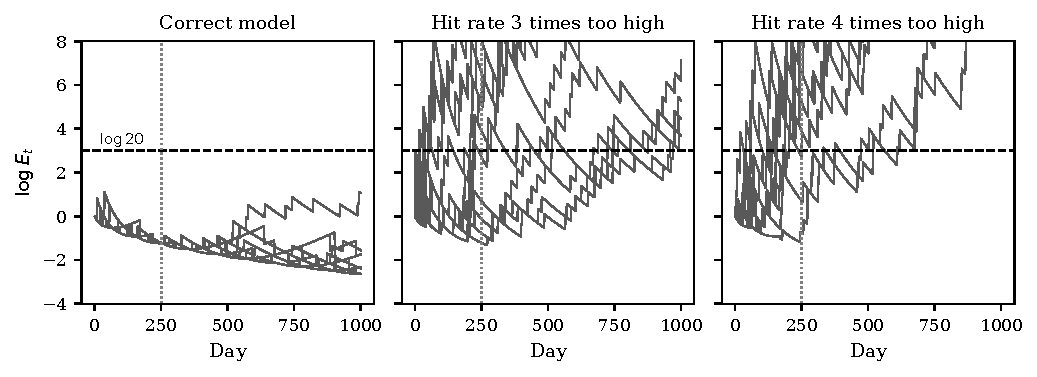
\includegraphics[width=\textwidth]{paths}
\caption{Twelve sample paths of $\log E_t$ of the rate e-process on streams of 1,000 days at a VaR level of 1\,\%: a correct model (left), a hit rate three times the nominal (middle) and four times (right). The dashed line is the rejection threshold $\log 20$ and the dotted line marks day 250, the first day a rule on the last 250 days can speak.}
\label{fig:paths}
\end{figure}

\Cref{tab:main-results} gives the size of every rule when it is read every day over 1,000 days. The rate e-process rejects a correct model in \nNullSizeE\,\% of the \nReps\ series (95\,\% interval \nNullSizeELo\ to \nNullSizeEHi\,\%) and the upper-side variant in \nNullSizeEUp\,\%, both under the acceptance bound of \nBound\,\%; the battery of the rate and clustering monitors in
\nNullSizeBattery\,\% and the clustering monitor alone in \nNullSizeCluster\,\%. The single-alternative likelihood ratio, which has a larger size because it is not spread over alternatives, is at \nNullSizeSprt\,\%, still under 5\,\%. The published e-backtest and the uniform-prior Bayes factor are at \nNullSizeWwz\ and \nNullSizeBeta\,\%. The proposed monitors are conservative, as a mixture
of martingales that starts at one and moves little on correct data should be: the observed size is well below the 5\,\% that \cref{prop:validity} allows. By contrast, the Kupiec test on the last 250 days rejects a correct model in \nNullSizeKupTrail\,\% of the series, the same test on all days so far in \nNullSizeKupCum\,\%, the traffic light leaves its green zone in \nNullSizeLight\,\%,
and the independence test on the last 250 days in \nNullSizeIndep\,\%. The Sidak-corrected Kupiec test controls size at the cost of power (\nNullSizeKupSidak\,\%), and the Kupiec test and the CUSUM with simulated thresholds are at \nNullSizeKupCal\ and \nNullSizeCusum\,\%, at the calibrated size, which the 20,000 calibration streams reproduce to within the
Monte Carlo error of $2{,}000$ streams (a standard error of about 0.5 points).

\begin{table*}[htbp]
\centering
\small
\caption{Every rule read every day on 2,000 streams of 1,000 days from the generator of known truth at a VaR level of 1\,\%: size is the share of correct-model streams rejected at some day, power by day 250 the share of streams with a hit rate three (x3) or four (x4) times too high rejected by day 250, and the median day is the median first-rejection day over all streams (the symbol $>$ marks a median beyond the horizon). Brackets are 95\,\% Wilson intervals for shares and 95\,\% bootstrap intervals for medians. The anytime bound for a size of 5\,\% plus three Monte Carlo standard errors is 6.5\,\%.}
\label{tab:main-results}
\resizebox{\linewidth}{!}{%
\begin{tabular}{p{5.6cm}rrrrr}
\toprule
Rule & Size, \% & Power by day 250, \% (x3) & Median day (x3) & Power by day 250, \% (x4) & Median day (x4) \\
\midrule
\relax Rate e-process, two-sided (proposed) & \relax 2.4 [1.8, 3.2] & \relax 48.6 [46.5, 50.8] & \relax 259 [237, 273] & \relax 77.8 [76.0, 79.6] & \relax 130 [125, 134] \\
\relax Rate e-process, upper side (proposed) & \relax 2.5 [1.9, 3.3] & \relax 55.4 [53.2, 57.5] & \relax 232 [221, 240] & \relax 82.5 [80.8, 84.1] & \relax 119 [108, 129] \\
\relax Single alternative, $3\alpha$ (likelihood-ratio e-process) & \relax 3.6 [2.9, 4.5] & \relax 62.5 [60.4, 64.6] & \relax 182 [176, 202] & \relax 86.1 [84.5, 87.5] & \relax 114 [111, 119] \\
\relax Rate and clustering e-processes, averaged (proposed) & \relax 1.2 [0.8, 1.8] & \relax 39.6 [37.5, 41.8] & \relax 320 [301, 332] & \relax 73.0 [71.0, 74.9] & \relax 158 [151, 161] \\
\relax E-backtest of Wang, Wang and Ziegel (2022) & \relax 0.4 [0.2, 0.8] & \relax 22.4 [20.6, 24.3] & \relax 408 [395, 422] & \relax 53.8 [51.6, 55.9] & \relax 237 [231, 246] \\
\relax Uniform-prior Bayes factor & \relax 0.8 [0.5, 1.3] & \relax 29.8 [27.8, 31.8] & \relax 433 [416, 462] & \relax 61.7 [59.5, 63.8] & \relax 200 [192, 206] \\
\relax Kupiec, last 250 days, read daily & \relax 65.7 [63.6, 67.7] & \relax 62.4 [60.2, 64.4] & \relax 250 [250, 250] & \relax 87.1 [85.6, 88.5] & \relax 250 [250, 250] \\
\relax Kupiec, all days so far, read daily & \relax 31.9 [29.9, 34.0] & \relax 79.0 [77.1, 80.7] & \relax 117 [110, 121] & \relax 94.2 [93.0, 95.1] & \relax 68 [66, 70] \\
\relax Basel traffic light, read daily & \relax 58.8 [56.6, 60.9] & \relax 87.0 [85.5, 88.4] & \relax 250 [250, 250] & \relax 97.2 [96.4, 97.8] & \relax 250 [250, 250] \\
\relax Kupiec, all days so far, Sidak level & \relax 0.1 [0.0, 0.3] & \relax 14.8 [13.3, 16.4] & \relax 567 [549, 581] & \relax 41.3 [39.2, 43.5] & \relax 286 [279, 302] \\
\relax Kupiec, all days so far, simulated critical value & \relax 5.3 [4.4, 6.4] & \relax 53.9 [51.8, 56.1] & \relax 239 [230, 245] & \relax 81.5 [79.7, 83.1] & \relax 130 [124, 135] \\
\relax CUSUM against $3\alpha$, simulated threshold & \relax 5.8 [4.9, 6.9] & \relax 46.0 [43.8, 48.2] & \relax 265 [256, 274] & \relax 76.5 [74.6, 78.3] & \relax 165 [159, 172] \\
\bottomrule
\end{tabular}}
\end{table*}


\Cref{fig:size-horizon} follows the share of correct models rejected as the horizon grows to \nHorizonDays\ days. It shows what \cref{tab:main-results} does not: that the size of a repeated rule is not a number but a function of the horizon. The Kupiec test on the last 250 days and the traffic light rise to \nHorizonEndKupTrail\,\% and \nHorizonEndLight\,\% and the Kupiec test on all days so far to \nHorizonEndKupCum\,\%,
as \cref{prop:repeated} says. The e-process reaches \nHorizonEndE\,\%, the e-backtest \nHorizonEndWwz\,\% and the Bayes factor \nHorizonEndBeta\,\% by day \nHorizonDays, under 5\,\% at every horizon, which is the guarantee that holds at any stopping time. The two rules calibrated to a size of 5\,\% over 1,000 days show the limit of a calibration: they are at
\nHorizonThousandKupCal\ and \nHorizonThousandCusum\,\% at day 1,000 and at \nHorizonEndKupCal\ and \nHorizonEndCusum\,\% at day \nHorizonDays. The figure does not say what a monitor detects; that is the subject of the next two subsections.

\begin{figure}[htbp]
\centering
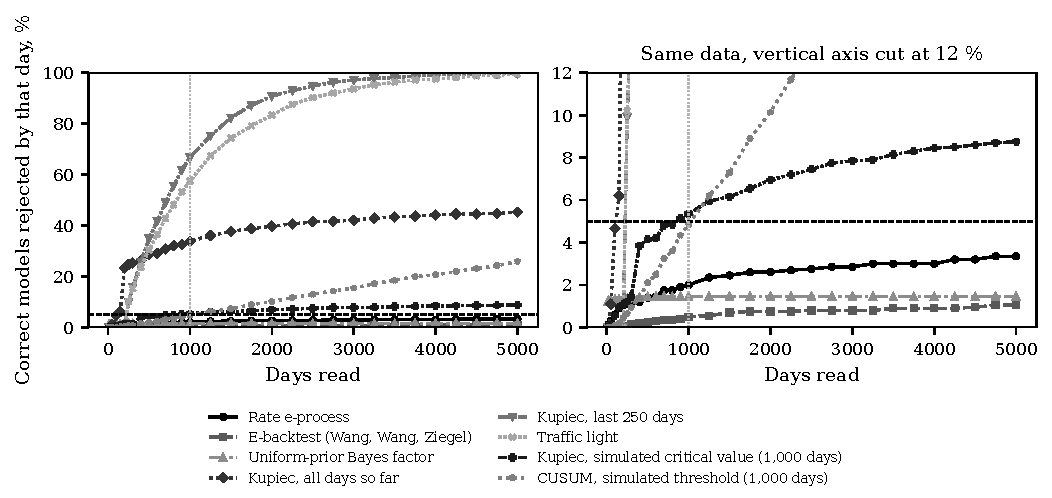
\includegraphics[width=\textwidth]{size-horizon}
\caption{Share of correct VaR models rejected by each rule as a function of the number of days read, from 2,000 streams of 5,000 days at a level of 1\,\% (left, full scale; right, the same curves with the vertical axis cut at 12\,\%). The dashed line is 5\,\% and the dotted line marks the 1,000-day horizon for which two of the rules were calibrated.}
\label{fig:size-horizon}
\end{figure}

\subsection{Detection delay}
\label{sec:results-delay}

\Cref{fig:delay-severity} plots the median first-rejection day and the power by day 250 against the hit-rate multiplier. All rules speed up as the departure grows, and the ranking at each severity is stable. At a hit rate four times the nominal the median day is \nMedFourE\ for the two-sided rate e-process (interval \nMedFourELo\ to \nMedFourEHi) and \nMedFourEUp\ for the upper-side
one, against \nMedFourSprt\ for the single alternative that knows the severity, \nMedFourKupCal\ for the Kupiec test with a simulated constant critical value, \nMedFourKupCum\ for the Kupiec test on all days so far (which has no size guarantee), and \nMedFourLight\ for the traffic light and for the Kupiec test on the last 250 days, which cannot speak before day 250. The published e-backtest
needs \nMedFourWwz\ days and the uniform-prior Bayes factor \nMedFourBeta. The mixture is therefore \nGapFourWwz\ days faster than the e-backtest at that severity (\nMedFourE\ against \nMedFourWwz) and \nGapThreeWwz\ days faster at three times the nominal (\nMedThreeE\ against \nMedThreeWwz), and about as fast as a simulation-calibrated boundary at four times the nominal, where the boundary has a size guarantee for 1,000 days only.

\begin{figure}[htbp]
\centering
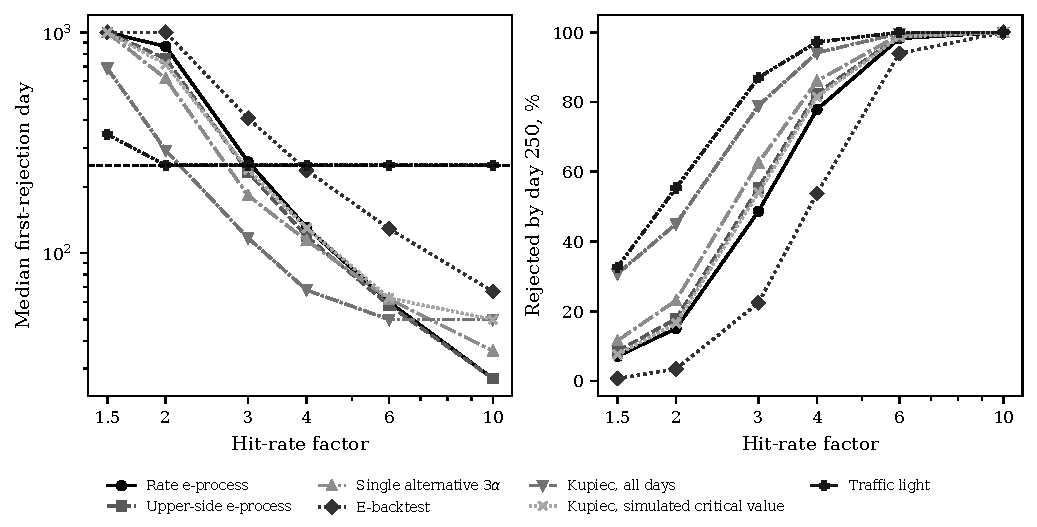
\includegraphics[width=\textwidth]{delay-severity}
\caption{Median first-rejection day (left, logarithmic axes; a point at 1,000 means the median is beyond the horizon) and share of streams rejected by day 250 (right) of the rate e-processes, the single-alternative e-process, the e-backtest and the repeated and calibrated fixed-window rules against the multiplier of the hit rate, 2,000 streams per point; the dashed line is the 250-day window.}
\label{fig:delay-severity}
\end{figure}

At a hit rate three times the nominal, the delay is on the edge of the window. In the main run the two-sided e-process has a median of \nMedThreeE\ days (interval \nMedThreeELo\ to \nMedThreeEHi). The committed document of the product, run with another seed, gives \nCommittedMedThree. \Cref{tab:x3-seeds} settles the question on \nSeedsCount\ independent seeds: the median of the pooled \nSeedsPooledN\ streams is \nSeedsThreeMed\ days (interval \nSeedsThreeMedLo\ to \nSeedsThreeMedHi), the median of single seeds has a mean of \nSeedsThreeSeedMean\ and a standard deviation of \nSeedsThreeSeedSd, and \nSeedsThreeBelow\,\% of the seeds
have a median below 250. The median delay of the two-sided monitor at a hit rate three times the nominal is therefore not distinguishable from the window, and it is not below the traffic light's median of \nSeedsThreeLight. At four times the nominal the pooled median is \nSeedsFourMed\ (interval \nSeedsFourMedLo\ to \nSeedsFourMedHi) and every seed is below 250. The upper-side monitor is below 250 at both severities, \nSeedsUpThreeMed\ days at three times (interval \nSeedsUpThreeMedLo\ to \nSeedsUpThreeMedHi) and \nSeedsUpFourMed\ at four.

\begin{table*}[htbp]
\centering
\small
\caption{The two-sided and the upper-side rate e-process at a hit rate three and four times too high on 20 independent seed sequences of 2,000 streams (40,000 streams per factor): the median first-rejection day of each seed with its mean and standard deviation, the share of seeds whose median is below the 250-day window, the median of the pooled streams with a bootstrap interval, the traffic-light median, and the power cost, the Kupiec power of one reading at day 250 minus the e-process power by day 250, pooled with its standard error and per seed with its standard deviation.}
\label{tab:x3-seeds}
\resizebox{\linewidth}{!}{%
\begin{tabular}{rrrrrrrr}
\toprule
Monitor, hit-rate factor & Mean of seed medians & SD of seed medians & Seeds with median below 250, \% & Pooled median [95\% CI] & Traffic-light median & Power cost, points ($\pm$ SE) & Per-seed power cost, points ($\pm$ SD) \\
\midrule
\relax Two-sided, 3 & 249.7 & 11.6 & \relax 45 & \relax 251.0 [247, 255] & 250 & \relax 12.4 $\pm$ 0.2 & \relax 12.4 $\pm$ 0.7 \\
\relax Two-sided, 4 & 127.7 & 2.7 & \relax 100 & \relax 128.0 [126, 129] & 250 & \relax 8.5 $\pm$ 0.2 & \relax 8.5 $\pm$ 0.7 \\
\relax Upper side, 3 & 227.8 & 6.7 & \relax 100 & \relax 228.0 [225, 231] & 250 & \relax 6.7 $\pm$ 0.2 & \relax 6.7 $\pm$ 0.7 \\
\relax Upper side, 4 & 110.8 & 4.8 & \relax 100 & \relax 109.0 [108, 110] & 250 & \relax 4.6 $\pm$ 0.1 & \relax 4.6 $\pm$ 0.6 \\
\bottomrule
\end{tabular}}
\end{table*}


The reading of the delay needs one caution, which the traffic light makes concrete. Its median of 250 is its first possible day: at three times the nominal it has flagged \nByThreeLight\,\% of the streams by day 250, and the e-process only \nByThreeE\,\%. A median below the window is a statement about the half of the streams detected earliest, not about the share detected by the end of the window.

\subsection{Power by day 250 and its cost}
\label{sec:results-power}

The power of the monitors by day 250 is the cost side of the guarantee. At a hit rate three times the nominal, the two-sided e-process rejects \nByThreeE\,\% of the streams by day 250 (the upper-side one \nByThreeEUp\,\%) against \nShotThree\,\% for one Kupiec reading at day 250 in the same streams; at four times the nominal, \nByFourE\,\% (\nByFourEUp\,\%) against \nShotFour\,\%.
The pooled power cost of the two-sided monitor is \nSeedsThreeCost\ $\pm$ \nSeedsThreeCostSe\ points at three times the nominal and \nSeedsFourCost\ $\pm$ \nSeedsFourCostSe\ points at four times, and that of the upper-side monitor \nSeedsUpThreeCost\ $\pm$ \nSeedsUpThreeCostSe\ and \nSeedsUpFourCost\ $\pm$ \nSeedsUpFourCostSe\ points (\cref{tab:x3-seeds}). The cost is below 10 points at four times the nominal for both monitors and at three times for the upper-side monitor only.

\Cref{tab:size-matched} and \cref{fig:power-size} put the cost in context. The Kupiec test at 250 days and a level of 1\,\% has an expected count of 2.5, so its two-sided size is \nExactKupSize\,\%, of which only \nExactKupUpperSize\,\% lies in the upper tail that rejects an understated VaR (it rejects from \nExactKupMinCount\ exceptions); the large lower-tail share is the probability of no exception in 250 days. The comparison of the monitor with the upper tail of the Kupiec test is therefore a comparison at a similar size, and
at three times the nominal the upper tail has a power of \nExactThreeKupUp\,\%. The most powerful test of the size the e-process spends by day 250 (\nExactESize\,\%) has a power of \nExactThreeNpE\,\% at three times the nominal: no rule with that spending can exceed it (\cref{prop:power}), and the two-sided e-process attains
\nByThreeE\,\% of the \nExactThreeNpE\,\% possible. The upper-side e-process spends more by day 250 (\nExactEUpSize\,\%), so its own bound is higher, \nExactThreeNpEUp\,\%, and it attains \nByThreeEUp\,\%. The cost of the guarantee is largely the cost of spending size over the later days: the mixture gives up power at day 250 to keep the size at every later day.

\begin{table*}[htbp]
\centering
\small
\caption{Exact power at day 250 and a VaR level of 1\,\% (expected count 2.5): the Kupiec test has a size of 9.5\,\% two-sided, of which 1.37\,\% lies in the upper tail that rejects an understated VaR (it rejects from 7 exceptions); the most powerful test, randomised, at the size 1.15\,\% that the rate e-process spends by day 250 on correct models bounds every test of that size; the last two columns are the measured shares of the e-processes on the generator.}
\label{tab:size-matched}
\resizebox{\linewidth}{!}{%
\begin{tabular}{rrrrrr}
\toprule
Hit-rate factor & Kupiec power, two-sided, \% & Kupiec power, upper tail, \% & Best test at the e-process size, \% & Rate e-process by day 250, \% [95\% CI] & Upper-side e-process by day 250, \% [95\% CI] \\
\midrule
\relax 2 & 24.3 & 23.6 & 21.2 & \relax 15.0 [13.5, 16.6] & \relax 17.8 [16.2, 19.5] \\
\relax 3 & 62.5 & 62.5 & 59.1 & \relax 48.6 [46.5, 50.8] & \relax 55.4 [53.2, 57.5] \\
\relax 4 & 87.5 & 87.5 & 85.5 & \relax 77.8 [76.0, 79.6] & \relax 82.5 [80.8, 84.1] \\
\relax 6 & 99.4 & 99.4 & 99.2 & \relax 98.2 [97.6, 98.7] & \relax 98.8 [98.2, 99.2] \\
\bottomrule
\end{tabular}}
\end{table*}


\begin{figure}[htbp]
\centering
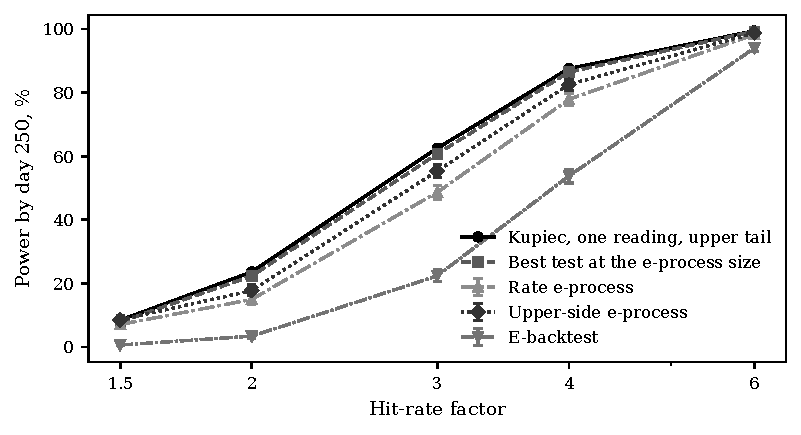
\includegraphics[width=0.85\textwidth]{power-size}
\caption{Power by day 250 against the multiplier of the hit rate at a level of 1\,\%: the exact power of the upper tail of one Kupiec reading, the exact power of the most powerful test at the size the rate e-process spends by day 250, and the measured power of the two-sided and the upper-side rate e-process and of the e-backtest with 95\,\% Wilson intervals, 2,000 streams per point.}
\label{fig:power-size}
\end{figure}

The first-order times of \cref{prop:growth} are compared with the measurements in \cref{tab:theory-delay} and \cref{fig:delay-theory}. The comparison needs the single alternative whose alternative is the true hit rate (the matched bet) at each factor, and the main run measured one single alternative only, the one at three times the nominal level, which is matched at that factor alone. The factors of the table were therefore run again with the matched single alternative on the same streams (an experiment of its own, \texttt{exp\_matched.py}). The matched likelihood ratio reaches the threshold in about \nKlSprtThree\ days at three times the nominal level and \nKlSprtFour\ at four, the mixture of eight alternatives in about \nKlMixThree\ and \nKlMixFour\ days; the measured medians are \nMatchedThreeMed\ and \nMatchedFourMed\ for the matched single alternative and \nMedThreeE\ and \nMedFourE\ for the mixture, all below the first-order times. At every factor from 2 to 10 the matched alternative is faster than the mixture (\nMatchedSixMed\ against \nMedSixE\ days at six times the nominal level and \nMatchedTenMed\ against \nMedTenE\ at ten times), the order of a matched and an unmatched bet that the theory predicts; the single alternative at three times the nominal level, which is matched at that factor only, is slower than the mixture at six and ten times (\nMedSixSprt\ and \nMedTenSprt\ days). The figure shows that the time grows as the inverse of the divergence, so the delay at a hit rate of 1.5 or 2 times the nominal is of the order of years: the mixture has a median of \nMedTwoE\ days at twice the nominal, and at 1.5 times more than half of the streams are not rejected within the 1,000 days (a median \nMedOneFiveE).

\begin{table*}[htbp]
\centering
\small
\caption{The first-order delay of the e-process at a VaR level of 1\,\%: the Kullback-Leibler divergence per day of the true hit rate from the null, in thousandths of a nat, the number of days a log-optimal bet needs to reach the threshold $\log 20$, the same with the penalty $\log K$ of a mixture of $K=8$ alternatives, and the measured median first-rejection days (95\,\% bootstrap intervals) of the single-alternative e-process whose alternative is the true hit rate (matched at every factor) and of the mixture e-process, on the same 2,000 streams. Where the median exceeds the 1,000-day horizon the symbol $>$ is printed.}
\label{tab:theory-delay}
\resizebox{\linewidth}{!}{%
\begin{tabular}{rrrrrr}
\toprule
Hit-rate factor $m$ & $1000\,\mathrm{KL}(m\alpha\|\alpha)$ & Time $\log 20/\mathrm{KL}$ & Time with the mixture penalty & Measured median, matched single alternative & Measured median, mixture \\
\midrule
\relax 1.5 & 1.09 & 2737 & 4636 & \relax $>$1,000 & \relax $>$1,000 \\
\relax 2 & 3.91 & 765 & 1297 & \relax 600 [584, 636] & \relax 862 [830, 920] \\
\relax 3 & 13.16 & 228 & 386 & \relax 182 [177, 203] & \relax 259 [237, 273] \\
\relax 4 & 25.91 & 116 & 196 & \relax 102 [95, 108] & \relax 130 [125, 134] \\
\relax 6 & 58.79 & 51 & 86 & \relax 45 [44, 46] & \relax 60 [58, 62] \\
\relax 10 & 144.48 & 21 & 35 & \relax 17 [16, 18] & \relax 27 [26, 28] \\
\bottomrule
\end{tabular}}
\end{table*}


\begin{figure}[htbp]
\centering
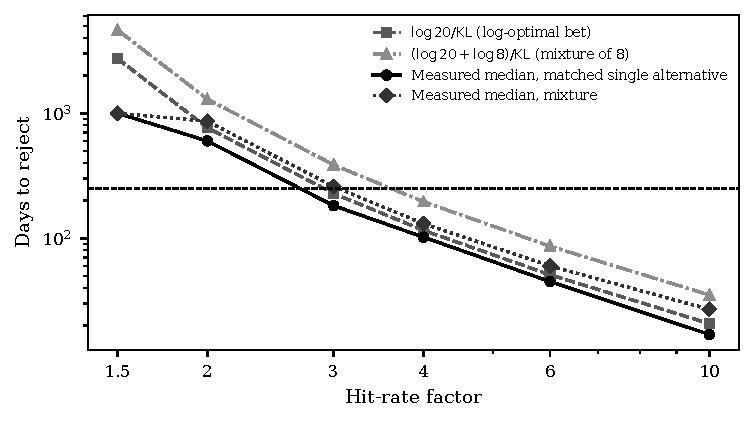
\includegraphics[width=0.8\textwidth]{delay-theory}
\caption{First-order times to reach the threshold $\log 20$ from \cref{prop:growth} (the matched likelihood ratio and the mixture of eight alternatives) and the measured median first-rejection days of the single-alternative and of the mixture e-process against the hit-rate multiplier at a level of 1\,\%; a point at 1,000 means a median beyond the horizon, and the dashed line is the 250-day window.}
\label{fig:delay-theory}
\end{figure}

\subsection{Hit clustering}
\label{sec:results-cluster}

A VaR with the right rate and clustered hits is the second departure. \Cref{tab:clustering} and \cref{fig:clustering} give the share of streams rejected. When hits follow hits with probability $0.4$ (forty times the unconditional rate), the clustering e-process rejects \nCluFourTenthCluster\,\% of the streams within 1,000 days (median \nCluMedFourTenthCluster\ days) and the battery of the two monitors \nCluFourTenthBattery\,\%, while the rate monitor alone rejects \nCluFourTenthE\,\%, more than its size of \nNullSizeE\,\%, because hits that follow hits break the conditional null of the rate monitor even when the rate is right. The Christoffersen test on the last 250 days reads the same departure faster, with a median of \nCluMedFourTenthIndep\ days and \nCluFourTenthIndep\,\% of streams, at a size of \nNullSizeIndep\,\% when it is read every day.
At $q=0.2$ the clustering e-process rejects \nCluTwoTenthCluster\,\% and at $q=0.1$ \nCluOneTenthCluster\,\%, so it is weak against mild clustering, with a median beyond the horizon at $0.1$. The traffic light and the Kupiec test on the last 250 days flag \nCluFourTenthLight\ and \nCluFourTenthKupTrail\,\% of the clustered streams, but they flag \nNullSizeLight\ and \nNullSizeKupTrail\,\% of the correct ones, so their rejection is no evidence of clustering. The Kupiec test with a simulated critical value rejects \nCluFourTenthKupCal\,\% of the clustered streams, because clustering at the right rate changes the count of hits in a window only through its variance.

\begin{table*}[htbp]
\centering
\small
\caption{Share of 1,000-day streams rejected at some day, in percent, when the hit rate is right (1\,\%) and a hit follows a hit with probability $q$ (0.1, 0.2, 0.4), for the proposed clustering monitors, the rate monitor and the fixed-window tests read daily. 2,000 streams per column; brackets are 95\,\% Wilson intervals. The first column is the size of each rule, the other three the power against clustering.}
\label{tab:clustering}
\resizebox{\linewidth}{!}{%
\begin{tabular}{p{6.2cm}rrrr}
\toprule
Rule & \relax Correct model & \relax $q=0.1$ & \relax $q=0.2$ & \relax $q=0.4$ \\
\midrule
\relax Clustering e-process (proposed) & \relax 0.5 [0.3, 0.9] & \relax 25.4 [23.6, 27.4] & \relax 53.8 [51.6, 56.0] & \relax 78.2 [76.3, 80.0] \\
\relax Rate and clustering, averaged (proposed) & \relax 1.2 [0.8, 1.8] & \relax 22.8 [21.0, 24.7] & \relax 51.6 [49.4, 53.8] & \relax 79.8 [78.0, 81.5] \\
\relax Rate e-process (proposed) & \relax 2.4 [1.8, 3.2] & \relax 4.9 [4.0, 5.9] & \relax 6.9 [5.9, 8.1] & \relax 18.6 [16.9, 20.3] \\
\relax Christoffersen independence, last 250 days, read daily & \relax 7.9 [6.8, 9.2] & \relax 57.5 [55.3, 59.6] & \relax 78.6 [76.7, 80.3] & \relax 91.6 [90.3, 92.7] \\
\relax Kupiec, last 250 days, read daily & \relax 65.7 [63.6, 67.7] & \relax 75.4 [73.5, 77.3] & \relax 83.3 [81.6, 84.9] & \relax 94.9 [93.8, 95.8] \\
\relax Basel traffic light, read daily & \relax 58.8 [56.6, 60.9] & \relax 62.8 [60.7, 64.9] & \relax 62.4 [60.3, 64.5] & \relax 68.3 [66.2, 70.3] \\
\relax Kupiec, all days so far, simulated critical value & \relax 5.3 [4.4, 6.4] & \relax 9.0 [7.8, 10.3] & \relax 13.4 [11.9, 14.9] & \relax 31.2 [29.3, 33.3] \\
\bottomrule
\end{tabular}}
\end{table*}


\begin{figure}[htbp]
\centering
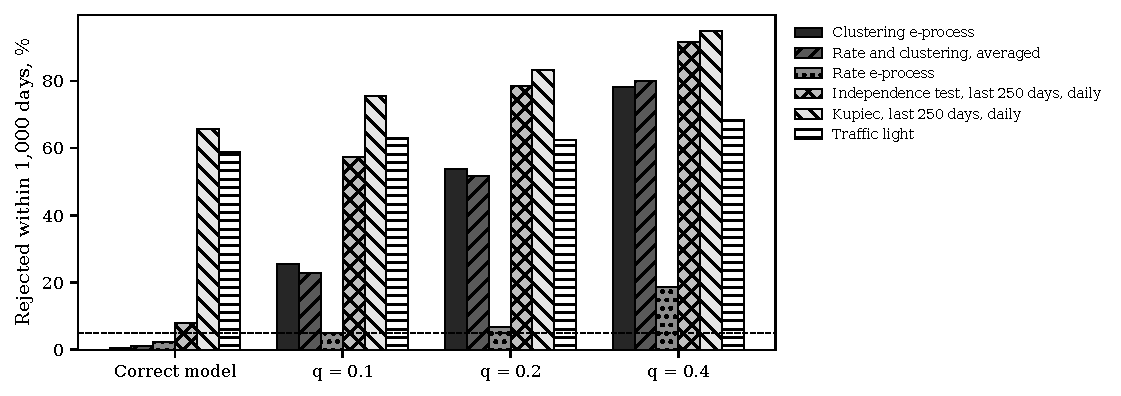
\includegraphics[width=0.9\textwidth]{clustering}
\caption{Share of streams of 1,000 days rejected at some day when the hit rate is right and a hit follows a hit with probability $q$, for the clustering and the rate e-processes, their average, the independence test and the Kupiec test on the last 250 days, the traffic light, each read every day, 2,000 streams per group; the first group is a correct model and the dashed line is 5\,\%.}
\label{fig:clustering}
\end{figure}

\subsection{Defaults against the PD of each grade}
\label{sec:results-pd}

\Cref{tab:pd-results} and \cref{fig:pd-books} (left) read the PD monitor on five grades over ten years. When the PD is right the product combination rejects \nPdOneProd\,\% and the average \nPdOneAvg\,\% of \nPdReps\ histories, while the chi-square test across grades read every year rejects \nPdOneChiEvery\,\%. When every PD is $1.1$ times the predicted one, the product rejects \nPdOneOneProd\,\%, the average \nPdOneOneAvg\,\% and the upper-side average \nPdOneOneAvgUp\,\% of the histories within ten years, while the chi-square test detects \nPdOneOneChiOne\,\% at year 10;
the median year of detection is \nPdMedYearOneOne\ for the upper-side average at that factor. At $1.05$ the monitors detect almost nothing (\nPdOneZeroFiveAvg\,\% for the average) against \nPdOneZeroFiveChiOne\,\% for the chi-square test at year 10. From $1.25$ every rule detects every history, the monitors at a median year of \nPdMedYearOneTwoFive. The size is held where the chi-square test read every year with its nominal critical value inflates it, but that is a property of the critical value and not of reading every year (a simulated critical value restores the size of the chi-square test and detects more, \cref{tab:pd-equal-size}), and the power cost for a small miscalibration is large: a ten-year cohort with a 5\,\% relative error in every grade is detected in \nPdOneZeroFiveChiOne\,\% of the histories by the chi-square test at year 10 and in \nPdOneZeroFiveAvgUp\,\% by the upper-side average e-process. The average detects more than the product at $1.1$ (\nPdOneOneAvg\ against \nPdOneOneProd\,\%), the reverse of what the independence assumed by the product would suggest;
\cref{sec:discussion} reads the difference through the growth-rate bound. When only the 10\,\% grade drifts (by $1.3$) every combination detects at least \nPdGradeProdUp\,\% of the histories (\cref{tab:ablation-pd}), so the average does not lose to the product where one grade carries the signal.

\begin{table*}[htbp]
\centering
\small
\caption{Defaults against the predicted PD of five grades (0.5 to 10\,\%), 2,000 obligors per grade and year, ten years, 1,000 histories per row from the generator of default counts: share of histories rejected at some year by the PD e-process combined by product or by average, by the chi-square test across grades on the cumulative counts read once at year 10, and by the same test read every year; the last column is the share of histories the upper-side average e-process rejects by year 3.}
\label{tab:pd-results}
\resizebox{\linewidth}{!}{%
\begin{tabular}{p{3.6cm}rrrrr}
\toprule
PD scaling & Product, \% & Average, \% & Chi-square at year 10, \% & Chi-square every year, \% & Average upper, by year 3, \% \\
\midrule
\relax 1 (size) & \relax 0.0 [0.0, 0.4] & \relax 0.4 [0.2, 1.0] & \relax 4.4 [3.3, 5.9] & \relax 20.8 [18.4, 23.4] & \relax 0.2 \\
\relax 1.05 & \relax 0.0 [0.0, 0.4] & \relax 2.9 [2.0, 4.1] & \relax 66.0 [63.0, 68.9] & \relax 78.7 [76.1, 81.1] & \relax 1.5 \\
\relax 1.1 & \relax 26.7 [24.1, 29.5] & \relax 55.9 [52.8, 58.9] & \relax 99.8 [99.3, 99.9] & \relax 99.8 [99.3, 99.9] & \relax 17.1 \\
\relax 1.25 & \relax 100.0 [99.6, 100.0] & \relax 100.0 [99.6, 100.0] & \relax 100.0 [99.6, 100.0] & \relax 100.0 [99.6, 100.0] & \relax 99.8 \\
\relax 10\% grade only, 1.3 & \relax 100.0 [99.6, 100.0] & \relax 100.0 [99.6, 100.0] & \relax 100.0 [99.6, 100.0] & \relax 100.0 [99.6, 100.0] & \relax 100.0 \\
\bottomrule
\end{tabular}}
\end{table*}


\Cref{tab:pd-correlation} and \cref{fig:pd-books} (right) show the effect \cref{prop:overdispersion} predicts. When the predicted PD is exactly right and the defaults of a year share a systematic factor, the two-sided e-processes reject \nRhoZeroThreeProd\,\% (product) and \nRhoZeroThreeAvg\,\% (average) of the histories at an asset correlation of $0.03$ and \nRhoOneTwoProd\ to \nRhoOneTwoAvg\,\% at $0.12$; the upper-side average rejects \nRhoZeroThreeAvgUp\,\% at $0.03$ and \nRhoTwoFourAvgUp\,\% at $0.24$. The chi-square test is not spared: it rejects \nRhoZeroThreeChiOne\,\% at year 10 and \nRhoZeroThreeChiEvery\,\% when read every year at $0.03$. At zero
correlation the sizes are those of \cref{tab:pd-results}. The loss is the loss of the binomial null that all these tests share, and the sequential construction inherits it and compounds it: the process grows by a factor above one in expectation at every year.

\begin{figure}[htbp]
\centering
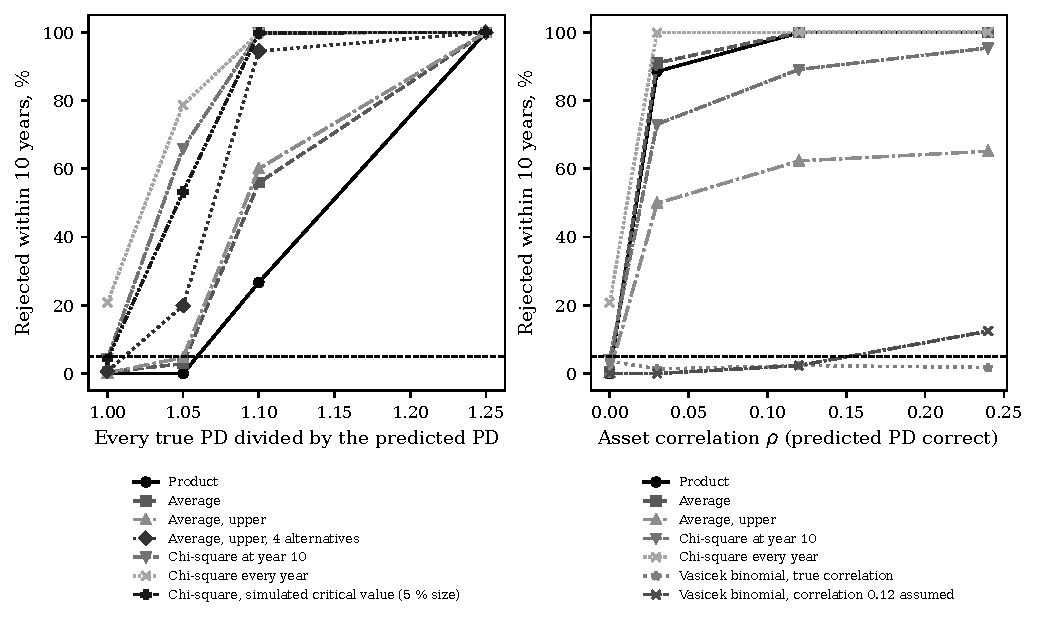
\includegraphics[width=\textwidth]{pd-books}
\caption{Share of ten-year histories of five rating grades rejected at some year. Left: every true PD is the predicted one multiplied by the factor on the horizontal axis, 1,000 histories per point, for the product and the average of the grade e-processes, the upper-side average with a coarse grid, and the chi-square test across grades. Right: the predicted PD is right and the defaults of each year share a systematic factor of asset correlation $\rho$, 2,000 histories per point, with the Vasicek-corrected binomial test of the engine at the true correlation and at an assumed correlation of 0.12; the dashed line is 5\,\%. The chi-square curve of the left panel uses a simulated critical value of size 5\,\%.}
\label{fig:pd-books}
\end{figure}

\begin{table*}[htbp]
\centering
\small
\caption{Share of 2,000 ten-year histories of five grades, with the predicted PD equal to the true PD, rejected at some year when the defaults of a year share one systematic factor of asset correlation $\rho$: the PD e-processes, whose null is binomial with no correlation, and the chi-square test across grades. The first row has no correlation and is the size under the null of both families.}
\label{tab:pd-correlation}
\resizebox{\linewidth}{!}{%
\begin{tabular}{rrrrrr}
\toprule
Asset correlation $\rho$ & Product, \% & Average, \% & Average, upper, \% & Chi-square at year 10, \% & Chi-square every year, \% \\
\midrule
\relax 0.00 & \relax 0.0 [0.0, 0.2] & \relax 0.6 [0.3, 1.0] & \relax 0.2 [0.1, 0.6] & \relax 4.2 [3.4, 5.1] & \relax 20.8 [19.0, 22.6] \\
\relax 0.03 & \relax 88.5 [87.0, 89.8] & \relax 91.0 [89.7, 92.2] & \relax 49.9 [47.7, 52.0] & \relax 73.0 [71.1, 74.9] & \relax 99.9 [99.6, 100.0] \\
\relax 0.12 & \relax 99.9 [99.6, 99.9] & \relax 100.0 [99.7, 100.0] & \relax 62.3 [60.2, 64.4] & \relax 89.1 [87.7, 90.4] & \relax 100.0 [99.8, 100.0] \\
\relax 0.24 & \relax 100.0 [99.8, 100.0] & \relax 100.0 [99.8, 100.0] & \relax 65.1 [63.0, 67.2] & \relax 95.4 [94.4, 96.2] & \relax 100.0 [99.8, 100.0] \\
\bottomrule
\end{tabular}}
\end{table*}


\Cref{tab:pd-comparators} runs the PD tests of the engine on the same histories. The exact binomial and the Jeffreys tests of each grade, read every year with a Bonferroni split, hold a size of \nPdcZeroBinEvery\ and \nPdcZeroJefEvery\,\% without correlation and reject \nPdcZeroThreeBinEvery\ and \nPdcZeroThreeJefEvery\,\% of the histories at an asset correlation of $0.03$, so they share the failure of the e-processes. The binomial test under the Vasicek one-factor mixture, which the engine carries as the remedy for correlated defaults, keeps its size when it is given the correlation that generated the histories: \nPdcZeroThreeVasTrueEvery\,\% at $0.03$, \nPdcOneTwoVasTrueEvery\,\% at $0.12$ and \nPdcTwoFourVasTrueEvery\,\% at $0.24$ (read once at year 10, \nPdcZeroThreeVasTrueOnce, \nPdcOneTwoVasTrueOnce\ and \nPdcTwoFourVasTrueOnce\,\%). With a correlation of \nPdcAssumedRho\ assumed it never rejects below that correlation (\nPdcZeroThreeVasAssumedEvery\,\% at $0.03$) and loses its size where the assumption is too low: \nPdcTwoFourVasAssumedEvery\,\% at $0.24$ (\nPdcTwoFourVasAssumedOnce\,\% read once). A comparator that holds its size under correlated defaults therefore exists, and the loss of size of the e-processes is not a consequence of reading every year; it is the consequence of a null without a correlation. The Vasicek test reads one year at a time and so does not pool the years as the e-process does; whether a monitor built on the same mixture would keep both the size and the pooling is the open step of \cref{sec:conclusions}.

\begin{table*}[htbp]
\centering
\small
\caption{The PD e-process and the PD tests of the engine on the same 2,000 histories as \cref{tab:pd-correlation} (predicted PD equal to the true PD, defaults of a year sharing a systematic factor of asset correlation $\rho$): share of histories rejected at some year, in percent with 95\,\% Wilson intervals. The per-grade tests (the exact binomial test, the Jeffreys test, and the binomial test under the Vasicek one-factor mixture with the correlation assumed or the true one) are one-sided; read every year they reject when any of the 5 grades in any of the 10 years has a p-value below $0.001$ (a Bonferroni split of 5\,\% over the 50 grade-years), and read once when any grade at year 10 is below $0.01$. The chi-square rule reads the statistic across grades every year against one critical value set by simulation on 50,000 correct histories to a size of 5\,\% over the ten years.}
\label{tab:pd-comparators}
\resizebox{\linewidth}{!}{%
\begin{tabular}{p{0.8cm}>{\raggedleft\arraybackslash}p{1.9cm}>{\raggedleft\arraybackslash}p{1.9cm}>{\raggedleft\arraybackslash}p{1.9cm}>{\raggedleft\arraybackslash}p{1.9cm}>{\raggedleft\arraybackslash}p{1.9cm}>{\raggedleft\arraybackslash}p{1.9cm}>{\raggedleft\arraybackslash}p{1.9cm}}
\toprule
$\rho$ & Average e-process & Binomial per grade & Jeffreys per grade & Vasicek, $0.12$ assumed & Vasicek, true $\rho$ & Vasicek, true $\rho$, read once & Chi-square, simulated critical value \\
\midrule
\relax 0.00 & \relax 0.6 [0.3, 1.0] & \relax 3.6 [2.9, 4.6] & \relax 4.1 [3.3, 5.1] & \relax 0.0 [0.0, 0.2] & \relax 3.6 [2.9, 4.6] & \relax 3.5 [2.7, 4.3] & \relax 4.4 [3.6, 5.4] \\
\relax 0.03 & \relax 91.0 [89.7, 92.2] & \relax 95.0 [94.0, 95.9] & \relax 95.3 [94.3, 96.1] & \relax 0.0 [0.0, 0.2] & \relax 1.4 [0.9, 2.0] & \relax 1.7 [1.2, 2.4] & \relax 99.2 [98.7, 99.5] \\
\relax 0.12 & \relax 100.0 [99.7, 100.0] & \relax 96.7 [95.8, 97.4] & \relax 96.8 [95.9, 97.4] & \relax 2.4 [1.8, 3.1] & \relax 2.4 [1.8, 3.1] & \relax 1.5 [1.1, 2.1] & \relax 100.0 [99.8, 100.0] \\
\relax 0.24 & \relax 100.0 [99.8, 100.0] & \relax 96.6 [95.7, 97.3] & \relax 96.7 [95.8, 97.4] & \relax 12.4 [11.1, 14.0] & \relax 1.8 [1.3, 2.4] & \relax 1.6 [1.1, 2.2] & \relax 100.0 [99.8, 100.0] \\
\bottomrule
\end{tabular}}
\end{table*}


The question the study asks of the PD monitor, whether the defaults of five grades are detected earlier than by the chi-square test read every year at an equal size, is answered by \cref{tab:pd-equal-size}. The chi-square test across grades is read every year against one constant critical value set by simulation on \nPdcCalReps\ correct histories, once to a size of 5\,\% over the ten years (a size of \nPdcOneChiSim\,\% on the histories of the table) and once to the size the average e-process measured, \nPdcMatchedSize\,\%. For a PD that is $5\,\%$ too low it rejects \nPdcOneZeroFiveChiSim\,\% of the histories within ten years (a median year of \nPdcOneZeroFiveChiSimYear) at the size of 5\,\% and \nPdcOneZeroFiveChiMatched\,\% at the size of the e-process, where the average e-process rejects \nPdOneZeroFiveAvg\,\%. For a PD that is $10\,\%$ too low the two chi-square rules reject \nPdcOneOneChiSim\,\% and \nPdcOneOneChiMatched\,\%, and \nPdcOneOneChiSimBy\ and \nPdcOneOneChiMatchedBy\,\% by year 3, against \nPdOneOneAvg\,\% and \nPdcOneOneAvgBy\,\% for the average e-process. From $1.25$ every rule rejects every history, the e-process at a median year of \nPdcOneTwoFiveAvgYear\ and the chi-square rules at \nPdcOneTwoFiveChiSimYear. At an equal size the defaults of the five grades are therefore not detected earlier by the e-process: on binomial defaults the chi-square rule detects a small miscalibration more often and sooner, and the e-process keeps what a simulated critical value lacks, a guarantee that does not depend on the horizon. The engine's per-grade binomial test, read every year with the Bonferroni split, detects \nPdcOneZeroFiveBinEvery\,\% at $1.05$ and \nPdcOneOneBinEvery\,\% at $1.1$.

\begin{table*}[htbp]
\centering
\small
\caption{Detection of a PD that is too low by the average PD e-process and by the chi-square test across grades read every year with a simulated constant critical value, at a size of 5\,\% and at the size the average e-process measured (0.4\,\%), on 1,000 histories per row (the histories of \cref{tab:pd-results}, no asset correlation). The first three rule columns give three numbers separated by slashes: the share of histories rejected within ten years (\%), the share rejected by year 3 (\%) and the median year of rejection among the histories rejected. The last two columns give the share rejected within ten years (\%) by the engine's binomial test per grade and by its Vasicek-corrected binomial test with a correlation of 0.12 assumed, each read every year with a Bonferroni split over the 50 grade-years.}
\label{tab:pd-equal-size}
\resizebox{\linewidth}{!}{%
\begin{tabular}{p{2.4cm}>{\raggedleft\arraybackslash}p{2.6cm}>{\raggedleft\arraybackslash}p{2.6cm}>{\raggedleft\arraybackslash}p{2.6cm}>{\raggedleft\arraybackslash}p{2.6cm}>{\raggedleft\arraybackslash}p{2.6cm}}
\toprule
PD scaling & Average e-process & Chi-square, 5\,\% size & Chi-square, size of the e-process & Binomial per grade, ever & Vasicek, $0.12$ assumed, ever \\
\midrule
\relax 1 (size) & \relax 0.4 / 0.4 / 1 & \relax 4.1 / 2.1 / 3 & \relax 0.4 / 0.2 / 4 & \relax 2.6 & \relax 0.0 \\
\relax 1.05 & \relax 2.9 / 0.8 / 4 & \relax 53.2 / 15.4 / 6 & \relax 23.2 / 2.4 / 7 & \relax 15.7 & \relax 0.0 \\
\relax 1.1 & \relax 55.9 / 13.8 / 6 & \relax 99.8 / 60.4 / 3 & \relax 98.8 / 29.3 / 5 & \relax 55.5 & \relax 0.0 \\
\relax 1.25 & \relax 100.0 / 99.7 / 2 & \relax 100.0 / 100.0 / 1 & \relax 100.0 / 100.0 / 1 & \relax 100.0 & \relax 0.0 \\
\relax 10\% grade only, 1.3 & \relax 100.0 / 100.0 / 1 & \relax 100.0 / 100.0 / 1 & \relax 100.0 / 100.0 / 1 & \relax 100.0 & \relax 0.0 \\
\bottomrule
\end{tabular}}
\end{table*}


\subsection{Real exceedances}
\label{sec:results-c11}

\Cref{tab:c11} reads the 18 models of the market-risk case at the 99\,\% level in the six windows. In the equity crisis of 2007 to 2009 every rule flags every model; the e-process flags them at a median day of \nCElevenEquityNinetyEMed, the Kupiec test on all days so far at \nCElevenEquityNinetyKupCumMed, and the traffic light at \nCElevenEquityNinetyLightMed (its first possible day). In the 2008 foreign-exchange window the e-process flags \nCElevenFxNinetyEFlag\ models at a median day of \nCElevenFxNinetyEMed, the traffic light \nCElevenFxNinetyLightFlag\ at day \nCElevenFxNinetyLightMed,
and the Kupiec test once at the end of the window \nCElevenFxNinetyKupEndFlag. Among the models the traffic light flags, the e-process misses \nCElevenFxNinetyLightMissedByE\ and flags the rest at a median day of \nCElevenFxNinetyLightE; it flags \nCElevenFxNinetyEOnlyVsKupiecEnd\ models that the end-of-window Kupiec test does not. In the window of 2020, with 104 days, the e-process flags \nCElevenCovidNinetyEFlag\ models at a median day of \nCElevenCovidNinetyEMed, and the traffic light cannot read the window at all; in 2022 (249 days), \nCElevenRatesNinetyEFlag\ at a median day of \nCElevenRatesNinetyEMed. In the 64 days of 2023 no rule flags any model.

\begin{table*}[htbp]
\centering
\small
\caption{The 18 models of the case on market risk in each of its six windows at the 99\,\% level: the number of models each rule flags at some day, and the median first-flag day among the models it flags. The rules are the rate e-process, the e-backtest of Wang, Wang and Ziegel (2022), the Kupiec test once at the end of the window (the eligibility gate), the Kupiec test on all days so far read daily from day 50, and the Basel traffic light, which needs 250 days (a dash where the window is shorter or the level is not the 99\,\% one). No truth is known in these windows.}
\label{tab:c11}
\resizebox{\linewidth}{!}{%
\begin{tabular}{lrrrrrrrrrr}
\toprule
Window & Days & Expected exceptions & E-process flags & Median day & E-backtest flags & Kupiec at end flags & Kupiec daily flags & Median day & Traffic light flags & Median day \\
\midrule
\relax calm-2004-06 & 750 & 7.5 & 2 & 352 & 1 & 3 & 7 & 70 & 9 & 252 \\
\relax equity-2007-09 & 504 & 5.0 & 18 & 24 & 18 & 18 & 18 & 50 & 18 & 250 \\
\relax fx-2008 & 251 & 2.5 & 9 & 68 & 7 & 7 & 18 & 68 & 11 & 250 \\
\relax equity-2020 & 104 & 1.0 & 12 & 25 & 6 & 13 & 13 & 50 & -- & -- \\
\relax rates-2022 & 249 & 2.5 & 8 & 52 & 3 & 8 & 17 & 54 & -- & -- \\
\relax mixed-2023 & 64 & 0.6 & 0 & -- & 0 & 0 & 0 & -- & -- & -- \\
\bottomrule
\end{tabular}}
\end{table*}


The calm window of 2004 to 2006 is the control: a quiet market in which the models should not be rejected systematically. The e-process flags \nCElevenCalmNinetyEFlag\ of the 18 models, the Kupiec test once at the end of the 750 days \nCElevenCalmNinetyKupEndFlag, and the e-backtest \nCElevenCalmNinetyWwzFlag; the rules read every day flag more: the Kupiec test on all days so far \nCElevenCalmNinetyKupCumFlag, the traffic light \nCElevenCalmNinetyLightFlag\ and the Kupiec test on the last 250 days \nCElevenCalmNinetyKupTrailFlag\ models. The 750 days give each of those rules
about three chances of an independent window, and the surplus of flags over the one-shot test is the repeated-reading inflation of \cref{prop:repeated} on real series, with the expected count of exceptions at the level in each model.
\Cref{fig:c11-days} compares the first flag of the e-process with that of the Kupiec test on all days so far for each model. In the crisis windows almost every model is flagged earlier by the e-process than the end of the window, and the Kupiec test on all days so far flags at the first look, day 50, in many models; in the calm window the points are few.

\begin{figure}[htbp]
\centering
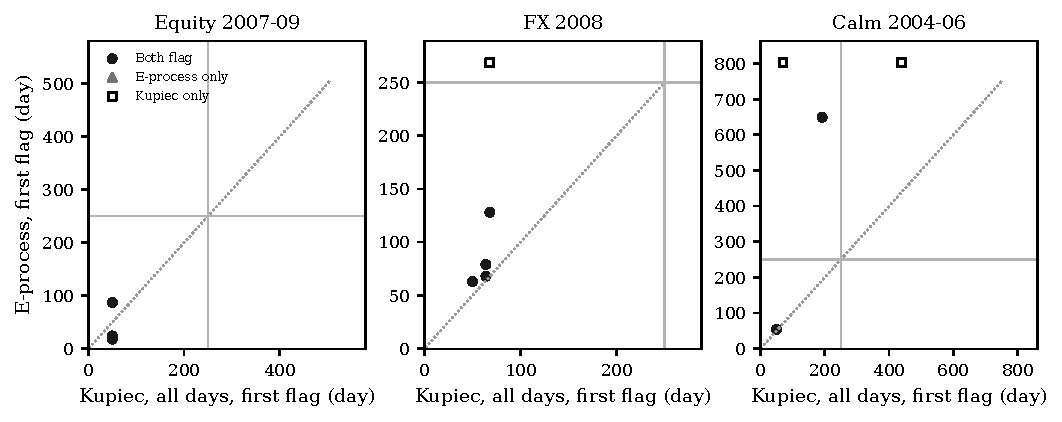
\includegraphics[width=\textwidth]{c11-days}
\caption{First day flagged by the rate e-process (vertical) against the first day flagged by the Kupiec test on all days so far (horizontal) for each of the 18 models at the 99\,\% level in three windows: the equity crisis, the foreign-exchange window of 2008 and the calm control window. Triangles on the right margin are models only the e-process flags and squares at the top are models only the Kupiec test flags; grey lines mark day 250.}
\label{fig:c11-days}
\end{figure}

At the 97.5\,\% level (\cref{tab:c11-975}) the e-process flags more models than the end-of-window Kupiec test in the windows of 2020 (\nCElevenCovidSeventyEFlag\ against \nCElevenCovidSeventyKupEndFlag), 2022 (\nCElevenRatesSeventyEFlag\ against \nCElevenRatesSeventyKupEndFlag) and 2008 (\nCElevenFxSeventyEFlag\ against \nCElevenFxSeventyKupEndFlag); in the calm window it flags fewer (\nCElevenCalmSeventyEFlag\ against \nCElevenCalmSeventyKupEndFlag). The comparison with the traffic light is
structurally in favour of the monitor, since the light cannot speak before day 250 and no rule of the set has a truth to be right against in these windows. The windows show when the rules fire, not which of them is right.

\begin{table*}[htbp]
\centering
\small
\caption{The 18 models of the case on market risk in each of its six windows at the 97.5\,\% level: the number of models each rule flags at some day, and the median first-flag day among the models it flags. The rules are the rate e-process, the e-backtest of Wang, Wang and Ziegel (2022), the Kupiec test once at the end of the window (the eligibility gate), the Kupiec test on all days so far read daily from day 50, and the Basel traffic light, which needs 250 days (a dash where the window is shorter or the level is not the 99\,\% one). No truth is known in these windows.}
\label{tab:c11-975}
\resizebox{\linewidth}{!}{%
\begin{tabular}{lrrrrrrrrrr}
\toprule
Window & Days & Expected exceptions & E-process flags & Median day & E-backtest flags & Kupiec at end flags & Kupiec daily flags & Median day & Traffic light flags & Median day \\
\midrule
\relax calm-2004-06 & 750 & 18.8 & 3 & 329 & 1 & 7 & 16 & 88 & -- & -- \\
\relax equity-2007-09 & 504 & 12.6 & 18 & 24 & 18 & 18 & 18 & 50 & -- & -- \\
\relax fx-2008 & 251 & 6.3 & 7 & 68 & 6 & 6 & 11 & 64 & -- & -- \\
\relax equity-2020 & 104 & 2.6 & 15 & 25 & 6 & 12 & 15 & 50 & -- & -- \\
\relax rates-2022 & 249 & 6.2 & 16 & 54 & 10 & 13 & 18 & 50 & -- & -- \\
\relax mixed-2023 & 64 & 1.6 & 0 & -- & 0 & 0 & 0 & -- & -- & -- \\
\bottomrule
\end{tabular}}
\end{table*}


\subsection{Real defaults by vintage}
\label{sec:results-c03}

\Cref{tab:c03} and \cref{fig:c03-paths} read the PD monitor on the five cohorts of small-business loans. The monitor looks for a vintage that defaults more than the predicted cumulative curve, with the vintages of a cohort as its grades and the ages as its steps, combined by average and by product. For the cohort of 2006 and 2007 and the cohort of 2008 to 2010 the monitor rejects at the first age, 12 months, with the largest value of $\log E$ of the average at \nCThreeMaxA\ and \nCThreeMaxB. The 2006 vintage has \nCThreeDTwoZeroZeroSix\ charge-offs against \nCThreePTwoZeroZeroSix\ predicted over the observed ages, the 2007 vintage \nCThreeDTwoZeroZeroSeven\ against \nCThreePTwoZeroZeroSeven. The binomial light read once at the five-year mark is red for these two vintages as well, 48 months later; the 2008 and 2009 vintages are red at the mark and rejected at 12 months, and the 2010 vintage is rejected at 24 months although its light is green and its charge-offs end below the predicted total (\nCThreeDTwoZeroOneZero\ against \nCThreePTwoZeroOneZero), a departure in the timing of the curve that a single reading at the mark does not see. No cohort from 2011 to 2020 is rejected as a cohort (the largest $\log E$ of an average is \nCThreeMaxE, below $\log 20=\nLogTwenty$): the model over-predicts, with for example \nCThreeDTwoZeroOneTwo\ charge-offs against \nCThreePTwoZeroOneTwo\ predicted in 2012, and a monitor of under-prediction has little to say. The 2018 vintage alone is rejected, at \nCThreeRejTwoZeroOneEight\ months ($\log E=\nCThreeVTwoZeroOneEight$), although its charge-offs end below the predicted total (\nCThreeDTwoZeroOneEight\ against \nCThreePTwoZeroOneEight); it is the same early-timing departure as the 2010 vintage, and the average over the three vintages of its cohort dilutes it. The values are the engine's output on the committed curves, recomputed here from the vintage curves with the product's builder and equal to the committed values for \nCThreeRebuilt\ of the five cohorts. Two to four vintages per cohort are few, and the binomial null has no asset correlation (\cref{prop:overdispersion}); the table illustrates the monitor on real curves and measures no power.

\begin{table*}[htbp]
\centering
\small
\caption{The PD e-process read at the ages 12, 24, 36, 48 and 60 months on the five cohorts of SBA 7(a) loans of the case on small-business credit, from the committed vintage curves: the charge-offs observed over the observed ages against the charge-offs the predicted curve implies, the first age at which each vintage and the cohort reject, and the light of the binomial test read once at the five-year mark. A dash means the monitor never reached 20.}
\label{tab:c03}
\resizebox{\linewidth}{!}{%
\begin{tabular}{llllllrr}
\toprule
Cohort & Vintages & Charge-offs / predicted & Month rejected, each & Five-year light, each & Month, average & Month, product & Largest $\log E$, average \\
\midrule
\relax FY2006-07 & \relax 2006, 2007 & \relax 19,271/7,601, 24,310/7,722 & \relax 12, 12 & \relax red, red & 12 & 12 & 11,631.0 \\
\relax FY2008-10 & \relax 2008, 2009, 2010 & \relax 13,088/4,526, 3,066/2,251, 1,954/2,158 & \relax 12, 12, 24 & \relax red, red, green & 12 & 12 & 6,362.5 \\
\relax FY2011-14 & \relax 2011, 2012, 2013, 2014 & \relax 1,662/2,957, 1,272/2,545, 1,240/2,506, 1,616/2,922 & \relax --, --, --, -- & \relax green, green, green, green & -- & -- & -2.5 \\
\relax FY2015-17 & \relax 2015, 2016, 2017 & \relax 2,134/4,886, 2,194/4,742, 2,417/4,508 & \relax --, --, -- & \relax green, green, green & -- & -- & -7.3 \\
\relax FY2018-20 & \relax 2018, 2019, 2020 & \relax 2,526/3,616, 1,786/2,630, 944/2,025 & \relax 12, --, -- & \relax green, green, green & -- & -- & 2.4 \\
\bottomrule
\end{tabular}}
\end{table*}


\begin{figure}[htbp]
\centering
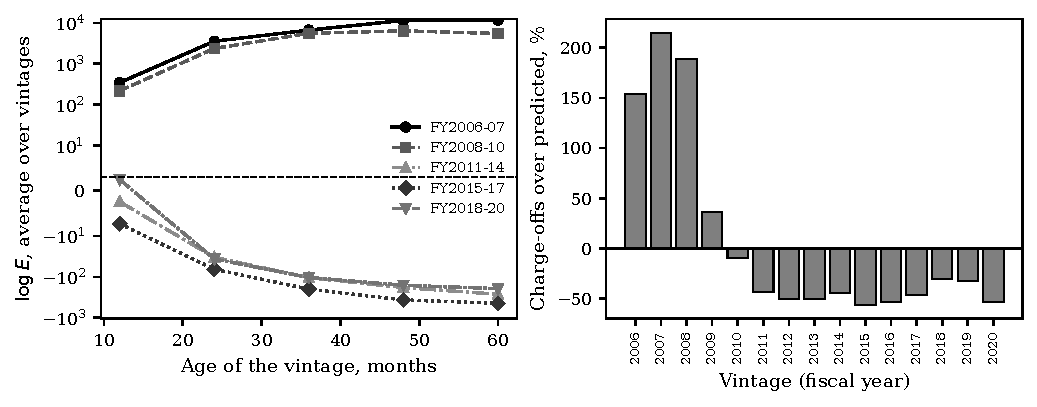
\includegraphics[width=\textwidth]{c03-paths}
\caption{Left: the log of the PD e-process averaged over the vintages of each cohort at the ages 12 to 60 months (symmetric logarithmic axis); the dashed line is the rejection threshold $\log 20$. Right: for each vintage, the charge-offs over the observed ages relative to the charge-offs of the predicted curve, in percent.}
\label{fig:c03-paths}
\end{figure}

\subsection{Agreement with the committed run and the outcome of the hypotheses}
\label{sec:results-agreement}

\Cref{tab:agreement} compares this study with the committed document of the product, which holds the same experiment from another seed. The shares ever rejected agree to within about one point (the Monte Carlo error of two runs of $2{,}000$ streams), and the median days agree to within the intervals of \cref{tab:main-results}, except the traffic light under clustering at $q=0.4$ (a median of \nCluMedFourTenthLight\ days in this run against \nCommittedCluMedFourTenthLight\ in the committed run); the committed medians at three and four times the nominal are \nCommittedMedThree\ and \nCommittedMedFour\ days, the power cost \nCommittedCostThree\ and \nCommittedCostFour\ points.
The committed document is also the product's own judgement of the hypotheses, and on one point this study reverses it. The document judges the delay hypothesis held at three times the nominal rate on one seed (a median of \nCommittedMedThree\ days against 250) and finds only the power cost failed (its verdict is that H3 failed and H1 and H2 held). On \nSeedsCount\ seeds the pooled median is \nSeedsThreeMed\ days (interval \nSeedsThreeMedLo\ to \nSeedsThreeMedHi), so that judgement of the delay does not survive replication; the spread of the median at three times the nominal in \cref{tab:x3-seeds} (a standard deviation of \nSeedsThreeSeedSd\ days between seeds) is of the size of the difference between the committed value and this run.

\begin{table*}[htbp]
\centering
\small
\caption{Agreement of this study with the committed document of the product (seed 42, 2,000 streams per scenario, same generator and engine release): the share of streams ever rejected and the median first-rejection day of three rules in four scenarios, the difference being the Monte Carlo error of two independent runs of 2,000 streams (about one point at the middle of the range).}
\label{tab:agreement}
\resizebox{\linewidth}{!}{%
\begin{tabular}{llrrrrr}
\toprule
Scenario & Rule & This run, ever, \% & Committed run, ever, \% & Difference, points & This run, median day & Committed run, median day \\
\midrule
\relax null & \relax Rate e-process & 2.4 & 1.8 & +0.6 & -- & -- \\
\relax null & \relax Kupiec, last 250 days & 65.7 & 66.5 & -0.8 & 718 & 704 \\
\relax null & \relax Traffic light & 58.8 & 58.7 & +0.1 & 812 & 840 \\
\relax rate x3 & \relax Rate e-process & 97.5 & 98.0 & -0.6 & 259 & 244 \\
\relax rate x3 & \relax Kupiec, last 250 days & 99.7 & 99.8 & -0.1 & 250 & 250 \\
\relax rate x3 & \relax Traffic light & 100.0 & 100.0 & +0.0 & 250 & 250 \\
\relax rate x4 & \relax Rate e-process & 100.0 & 100.0 & +0.0 & 130 & 129 \\
\relax rate x4 & \relax Kupiec, last 250 days & 100.0 & 100.0 & +0.0 & 250 & 250 \\
\relax rate x4 & \relax Traffic light & 100.0 & 100.0 & +0.0 & 250 & 250 \\
\relax cluster 0.4 & \relax Rate e-process & 18.6 & 18.2 & +0.4 & -- & -- \\
\relax cluster 0.4 & \relax Kupiec, last 250 days & 94.9 & 95.0 & -0.2 & 357 & 365 \\
\relax cluster 0.4 & \relax Traffic light & 68.3 & 66.8 & +1.5 & 622 & 670 \\
\bottomrule
\end{tabular}}
\end{table*}


\Cref{tab:hypotheses} gives the outcome of each hypothesis. H1 holds: the size is held and the repeated Kupiec rule exceeds it. H2 holds at four times the nominal and above and does not hold at three times for the two-sided monitor, whose pooled median is \nSeedsThreeMed\ days (interval \nSeedsThreeMedLo\ to \nSeedsThreeMedHi) against the 250 of the window and of the traffic light. H3 holds at four times the nominal and
fails at three times for the two-sided monitor (\nSeedsThreeCost\ points). The refutation clause, as the design states it on the equity and foreign-exchange windows, does not fire: the median day of the e-process among the models the traffic light flags is \nCElevenEquityNinetyLightE\ against \nCElevenEquityNinetyLightDay\ and \nCElevenFxNinetyLightE\ against \nCElevenFxNinetyLightDay. The same comparison on the generator, which this study adds to the clause, is the delay criterion of H2 and is reported there: at three times the nominal rate the pooled median, \nSeedsThreeMed, is not below the traffic light's \nSeedsThreeLight. The hypotheses as stated therefore do not hold as a whole: the delay and the power cost fail at three times the nominal rate and hold at four. The PD prediction is confirmed (\cref{sec:results-pd}). Two results were not pre-stated. The upper-side variant, which was chosen after the two-sided results, meets the delay and the power criteria at both severities on the same \nSeedsPooledN\ streams per factor; the choice is a finding that a prospective test would confirm, not a result of the pre-stated design. The PD question, whether the defaults of five grades are detected earlier than by the chi-square test at an equal size, was run after the other results and is answered no (\cref{sec:results-pd}).

\begin{table*}[htbp]
\centering
\small
\caption{The hypotheses of the proposed monitors, stated before the experiments, with the measurements that judge them and the outcome of each: size on the generator of known truth, delay and power cost pooled over 20 independent seeds of 2,000 streams, and the refutation clause on the generator and on the two real windows of the case on market risk at the 99\,\% level.}
\label{tab:hypotheses}
\resizebox{\linewidth}{!}{%
\begin{tabular}{p{6.0cm}p{6.6cm}p{2.4cm}}
\toprule
Hypothesis, stated before the experiments & Measured & Outcome \\
\midrule
\relax Size: the e-process rejects a correct VaR in at most $5\,\%$ plus three standard errors of the streams, read daily over 1,000 days, where the repeated Kupiec rule exceeds that & \relax e-process 2.4\,\%; Kupiec last 250 days 65.7\,\%, all days 31.9\,\%; bound 6.5\,\% & Held \\
\relax Delay: the median detection day is below the 250-day window, and below the traffic light's, at a hit rate three and four times too high & \relax x3: pooled median 251 [247, 255] (traffic light 250); 45\,\% of seeds below 250. x4: 128 [126, 129] (traffic light 250) & \relax x3: not met; x4: held \\
\relax Power cost: one Kupiec reading at day 250 has less than 10 points more power than the e-process has by day 250 & \relax x3: 12.4 $\pm$ 0.2 points; x4: 8.5 $\pm$ 0.2 points & \relax x3: not met; x4: held \\
\relax Upper-side variant of the rate monitor (chosen after the two-sided results, the direction a supervisor penalises): delay below 250 and below the traffic light's, and power cost under 10 points & \relax x3: pooled median 228 [225, 231], cost 6.7 $\pm$ 0.2 points; x4: 109 [108, 110], cost 4.6 $\pm$ 0.1 points & \relax Met at both severities \\
\relax Refutation clause: the hypothesis is refuted if the delay is not lower than the traffic light's, on the generator and on the equity 2007 to 2009 and foreign-exchange 2008 windows & \relax generator: x3 251 against 250, x4 128 against 250; real windows (models the light flags): median day 24 against 250 and 68 against 250 & \relax Fires at x3; not at x4 or on the real windows \\
\bottomrule
\end{tabular}}
\end{table*}


\section{Ablation}
\label{sec:ablation}

Each component of the proposed monitors is removed or replaced in turn on the same generators, with one change at a time and the same streams for every variant of a scenario, so that the differences within a table are paired and smaller than the differences between runs. The three tables below are the ablation: \cref{tab:ablation-grid} for the mixture of the rate monitor, \cref{tab:ablation-battery} for the combination of the two VaR monitors,
and \cref{tab:ablation-pd} for the PD monitor.

\subsection{The mixture over alternative hit rates}
\label{sec:ablation-mixture}

\Cref{tab:ablation-grid} replaces the full grid by single alternatives and by parts of the grid. A single alternative is the likelihood-ratio e-process of one hit rate and is the monitor that the theory says is fastest when its alternative is the truth. At a hit rate three times the nominal, the single alternative at $3\alpha$ has a median of \nAbMedThreeSingleThree\ days and \nAbByThreeSingleThree\,\% power by day 250,
and at four times the nominal the one at $4\alpha$ has \nAbMedFourSingleFour\ days and \nAbByFourSingleFour\,\%; against them the full grid has \nAbMedThreeFull\ days and \nAbByThreeFull\,\% at three times and \nAbMedFourFull\ days and \nAbByFourFull\,\% at four times. The difference is the price of not knowing the severity. A single alternative that is far from the truth is worse than the mixture: the alternative at $10\alpha$ has a median beyond the horizon at three times
the nominal (\nAbMedThreeSingleTen) and only \nAbByThreeSingleTen\,\% power by day 250, and the alternative at $1.5\alpha$ has \nAbByThreeSingleOneFive\,\% there.

Cutting the grid shows which alternatives carry the power. Dropping the two alternatives below the nominal level (the upper half) raises the power by day 250 at three times the nominal from \nAbByThreeFull\ to \nAbByThreeUpper\,\% and lowers the median from \nAbMedThreeFull\ to \nAbMedThreeUpper\ days at no visible cost in size (\nAbNullFull\ and \nAbNullUpper\,\%), because the weight on the alternatives that point the other way is wasted when the departure is upward.
Keeping only the alternatives $1.5$ to $4$ gives \nAbByThreeUpperLow\,\% at three times the nominal and, among the cuts of the grid, the best power against twice the nominal (\nAbEverTwoUpperLow\,\% rejected within 1,000 days), while keeping only $3$ to $10$ gives the fastest delays at four and six times and loses power at twice the nominal (\nAbEverTwoUpperHigh\,\%). The grid trades breadth of coverage against speed at a given severity, and no cut dominates; the full grid is the choice that does not prejudge the severity or the direction.

\begin{table*}[htbp]
\centering
\small
\caption{Ablation of the mixture over alternative hit rates of the rate monitor on 2,000 streams of 1,000 days per scenario: the full grid, its upper half, the upper half cut at its low and high ends, and each single alternative, which is the likelihood-ratio e-process of one hit rate. Size and power (x2) are shares ever rejected; power by day 250 and median days are for hit rates three (x3), four (x4) and six (x6) times too high; brackets are 95\,\% intervals.}
\label{tab:ablation-grid}
\resizebox{\linewidth}{!}{%
\begin{tabular}{p{4.4cm}rrrrrrr}
\toprule
Mixture grid & Size, \% & Power x2, \% & Power by 250 x3, \% & Median day x3 & Power by 250 x4, \% & Median day x4 & Median day x6 \\
\midrule
\relax Full two-sided grid, $0.25$ to $10$ & \relax 2.2 [1.7, 3.0] & \relax 55.8 [53.6, 58.0] & \relax 52.3 [50.1, 54.5] & \relax 232 [220, 249] & \relax 77.8 [75.9, 79.6] & \relax 128 [121, 133] & \relax 58 [56, 60] \\
\relax Upper half, $1.5$ to $10$ & \relax 2.4 [1.8, 3.2] & \relax 59.2 [57.1, 61.4] & \relax 57.1 [54.9, 59.3] & \relax 215 [194, 226] & \relax 82.0 [80.2, 83.6] & \relax 108 [105, 120] & \relax 56 [54, 58] \\
\relax Upper alternatives $1.5$ to $4$ & \relax 2.6 [2.0, 3.4] & \relax 64.4 [62.3, 66.5] & \relax 57.4 [55.2, 59.6] & \relax 207 [199, 214] & \relax 82.5 [80.8, 84.2] & \relax 120 [110, 130] & \relax 60 [59, 62] \\
\relax Upper alternatives $3$ to $10$ & \relax 3.0 [2.4, 3.9] & \relax 53.4 [51.3, 55.6] & \relax 59.3 [57.1, 61.4] & \relax 191 [180, 203] & \relax 83.1 [81.4, 84.7] & \relax 104 [99, 107] & \relax 50 [42, 53] \\
\relax Single alternative $1.5\alpha$ & \relax 0.9 [0.5, 1.4] & \relax 59.5 [57.3, 61.6] & \relax 18.2 [16.6, 20.0] & \relax 381 [374, 406] & \relax 46.6 [44.4, 48.7] & \relax 261 [255, 267] & \relax 154 [150, 158] \\
\relax Single alternative $2\alpha$ & \relax 2.9 [2.3, 3.7] & \relax 72.5 [70.6, 74.5] & \relax 51.9 [49.7, 54.1] & \relax 245 [239, 251] & \relax 78.7 [76.9, 80.4] & \relax 162 [158, 167] & \relax 95 [93, 96] \\
\relax Single alternative $3\alpha$ & \relax 3.3 [2.6, 4.2] & \relax 63.3 [61.2, 65.4] & \relax 64.0 [61.9, 66.1] & \relax 175 [170, 181] & \relax 86.4 [84.8, 87.8] & \relax 110 [106, 114] & \relax 60 [59, 62] \\
\relax Single alternative $4\alpha$ & \relax 3.0 [2.4, 3.9] & \relax 48.1 [46.0, 50.3] & \relax 63.0 [60.9, 65.1] & \relax 167 [159, 173] & \relax 85.2 [83.6, 86.7] & \relax 99 [91, 105] & \relax 55 [53, 56] \\
\relax Single alternative $10\alpha$ & \relax 2.0 [1.5, 2.7] & \relax 14.4 [12.9, 16.0] & \relax 38.5 [36.4, 40.7] & \relax $>$1,000 & \relax 63.9 [61.8, 66.0] & \relax 117 [108, 135] & \relax 42 [40, 43] \\
\bottomrule
\end{tabular}}
\end{table*}


\subsection{The direction of the alternatives}
\label{sec:ablation-direction}

The upper half of the grid is the one-sided monitor of a supervisor, who penalises a VaR that understates the risk and does not penalise one that is too conservative. It is the cheapest change in \cref{tab:ablation-grid}, and it is the one that moves the hypotheses. On the pooled \nSeedsPooledN\ streams per factor of \cref{tab:x3-seeds} the upper-side monitor has a median of \nSeedsUpThreeMed\ days at three times the nominal level against \nSeedsThreeMed\ for the two-sided one, and a power cost of \nSeedsUpThreeCost\ points against \nSeedsThreeCost;
at four times the nominal, \nSeedsUpFourMed\ days against \nSeedsFourMed\ and \nSeedsUpFourCost\ points against \nSeedsFourCost. The upper-side monitor rejects a correct model in \nNullSizeEUp\,\% of the main-run series, against \nNullSizeE\,\% for the two-sided one: its size is not larger in any way that matters. The price is that it has no power against a model that is too conservative, which the supervisory test does not ask for and a validator of the efficiency of a model may; for that validator the two-sided monitor is the choice, and its delay at a hit rate below the nominal is not measured here.

\subsection{The combination of the two VaR monitors}
\label{sec:ablation-battery}

\Cref{tab:ablation-battery} runs the rate monitor, the clustering monitor, their average, the union of the two at a threshold of 40 each (the Bonferroni split of the size, valid by the union bound) and their product on the same streams. The average and the union are valid and almost identical: they reject \nAbBatThreeAverage\ and \nAbBatThreeUnion\,\% of the streams with a hit rate three times too high, against \nAbBatThreeRate\,\% for the rate monitor alone, and \nAbBatClFourAverage\ and \nAbBatClFourUnion\,\% of the streams with clusters at $q=0.4$, against
\nAbBatClFourCluster\,\% for the clustering monitor alone. Averaging two monitors costs at most the factor two on each, and it buys the detection of either departure, which neither monitor has alone. The product is not an e-process for two monitors of one stream (\cref{prop:product}), but its measured size at a level of 1\,\% is \nAbBatNullProduct\,\%: the rate monitor and the clustering monitor rarely move together on a correct model at that level, so the invalidity does not show at 1\,\% and does show at the level of
$0.2$ of the enumeration (\cref{tab:null-expectation}). The product detects \nAbBatClFourProduct\,\% at $q=0.4$, about the same as the average (\nAbBatClFourAverage\,\%), so nothing is gained by taking the risk.

\begin{table*}[htbp]
\centering
\small
\caption{Ablation of the combination of the two VaR monitors that read the same stream, on 2,000 streams of 1,000 days per scenario: share of streams ever rejected, in percent, when the model is right (size), when the hit rate is three times too high, and when hits cluster at the right rate. The product is shown to measure its size, which the theory does not bound.}
\label{tab:ablation-battery}
\resizebox{\linewidth}{!}{%
\begin{tabular}{p{5.4cm}rrrrr}
\toprule
Combination & Size, \% & Rate x3, \% & Clustering $q=0.2$, \% & Clustering $q=0.4$, \% & Median day, $q=0.4$ \\
\midrule
\relax Rate e-process & \relax 1.8 [1.3, 2.5] & \relax 97.5 [96.8, 98.1] & \relax 7.5 [6.4, 8.7] & \relax 18.1 [16.5, 19.9] & \relax $>$1,000 \\
\relax Clustering e-process & \relax 0.4 [0.2, 0.9] & \relax 8.6 [7.4, 9.9] & \relax 53.3 [51.2, 55.5] & \relax 77.2 [75.4, 79.0] & \relax 525 [491, 556] \\
\relax Average of the two (battery, valid) & \relax 1.2 [0.8, 1.8] & \relax 96.4 [95.5, 97.1] & \relax 51.6 [49.5, 53.8] & \relax 78.8 [77.0, 80.6] & \relax 523 [487, 554] \\
\relax Either at threshold 40 (union, valid) & \relax 1.2 [0.8, 1.8] & \relax 96.4 [95.4, 97.1] & \relax 51.6 [49.5, 53.8] & \relax 78.8 [77.0, 80.5] & \relax 525 [491, 557] \\
\relax Product of the two (not an e-process on one stream) & \relax 2.5 [1.9, 3.2] & \relax 95.5 [94.4, 96.3] & \relax 48.8 [46.6, 50.9] & \relax 79.0 [77.1, 80.7] & \relax 474 [445, 506] \\
\bottomrule
\end{tabular}}
\end{table*}


\subsection{The PD monitor: combination, direction and grid}
\label{sec:ablation-pd}

\Cref{tab:ablation-pd} varies the combination of the grades, the direction and the grid of the PD monitor. With the PD right, none of the monitors rejects more than \nPdOneSingle\,\% of the histories; the chi-square test read once at year 10 is at \nPdOneChiOne\,\% and read every year at \nPdOneChiEvery\,\%. With every PD multiplied by $1.1$, the combination by product rejects \nPdOneOneProd\,\%, by average \nPdOneOneAvg\,\%, and the upper-side average \nPdOneOneAvgUp\,\% of the histories, so the direction and the combination matter little against the grid. The grid matters a great deal: with four alternatives between $1.1$ and $2$ instead of the
sixteen of the default, the upper-side average rejects \nPdOneOneCoarse\,\% of the histories at $1.1$ and \nPdOneZeroFiveCoarse\,\% at $1.05$, against \nPdOneOneAvgUp\ and \nPdOneZeroFiveAvgUp\,\%, with a size of \nPdOneCoarse\,\%. A single alternative at $1.25$ gives \nPdOneOneSingle\,\% at $1.1$. The default grid spreads the weight over alternatives far from the departures that a small relative error produces: half of its upper alternatives are above $2$, and
\cref{prop:growth} says that a mixture pays the logarithm of the number of alternatives it does not need. The coarse grid still detects less than the chi-square rule at a nominal size of 5\,\% (\nPdcOneOneChiSim\,\% at $1.1$ and \nPdcOneZeroFiveChiSim\,\% at $1.05$; \cref{tab:pd-equal-size}). A validator who knows the range of miscalibrations of interest can set a coarse grid before the data and gain power at no cost in size; the default of the engine was fixed before these experiments and is not changed here.

\begin{table*}[htbp]
\centering
\small
\caption{Ablation of the PD monitor of five grades over ten years on 1,000 histories per column from the generator of default counts with no asset correlation: share of histories ever rejected, in percent with 95\,\% Wilson intervals, for the grades combined by product or by average, two-sided or upper, with coarser grids, and for the chi-square test across grades read once or every year.}
\label{tab:ablation-pd}
\resizebox{\linewidth}{!}{%
\begin{tabular}{p{5.8cm}rrrrr}
\toprule
Rule & Every PD right (size) & Every PD $\times 1.05$ & Every PD $\times 1.1$ & Every PD $\times 1.25$ & 10\,\% grade $\times 1.3$ \\
\midrule
\relax Product, two-sided & \relax 0.0 [0.0, 0.4] & \relax 0.0 [0.0, 0.4] & \relax 26.7 [24.1, 29.5] & \relax 100.0 [99.6, 100.0] & \relax 100.0 [99.6, 100.0] \\
\relax Product, upper & \relax 0.0 [0.0, 0.4] & \relax 0.0 [0.0, 0.4] & \relax 28.4 [25.7, 31.3] & \relax 100.0 [99.6, 100.0] & \relax 99.9 [99.4, 100.0] \\
\relax Average, two-sided & \relax 0.4 [0.2, 1.0] & \relax 2.9 [2.0, 4.1] & \relax 55.9 [52.8, 58.9] & \relax 100.0 [99.6, 100.0] & \relax 100.0 [99.6, 100.0] \\
\relax Average, upper & \relax 0.2 [0.1, 0.7] & \relax 4.7 [3.6, 6.2] & \relax 60.0 [56.9, 63.0] & \relax 100.0 [99.6, 100.0] & \relax 100.0 [99.6, 100.0] \\
\relax Average, upper, four alternatives $1.1$ to $2$ & \relax 0.7 [0.3, 1.4] & \relax 19.9 [17.5, 22.5] & \relax 94.5 [92.9, 95.8] & \relax 100.0 [99.6, 100.0] & \relax 100.0 [99.6, 100.0] \\
\relax Average, upper, one alternative $1.25$ & \relax 0.9 [0.5, 1.7] & \relax 9.7 [8.0, 11.7] & \relax 60.0 [56.9, 63.0] & \relax 100.0 [99.6, 100.0] & \relax 100.0 [99.6, 100.0] \\
\relax Chi-square across grades, read once at year 10 & \relax 4.4 [3.3, 5.9] & \relax 66.0 [63.0, 68.9] & \relax 99.8 [99.3, 99.9] & \relax 100.0 [99.6, 100.0] & \relax 100.0 [99.6, 100.0] \\
\relax Chi-square across grades, read every year & \relax 20.8 [18.4, 23.4] & \relax 78.7 [76.1, 81.1] & \relax 99.8 [99.3, 99.9] & \relax 100.0 [99.6, 100.0] & \relax 100.0 [99.6, 100.0] \\
\bottomrule
\end{tabular}}
\end{table*}


\section{Discussion}
\label{sec:discussion}

\subsection{Why the results are what they are}
\label{sec:discussion-why}

Three mechanisms account for the measurements. The first is the spending of size. A fixed-window test spends its whole size at one reading; a monitor that is valid at every time spends it over all days, and by day 250 the rate e-process has spent about \nExactESize\,\% of a nominal 5\,\%. \Cref{prop:power} turns that into a bound on the power by day 250, and the measured power sits under the bound: \nByThreeE\,\% against a bound of \nExactThreeNpE\,\% at three times the nominal.
The power cost is therefore largely the consequence of the guarantee and not of a poor design; what design can change is how much of the bound is attained, and the single alternative at the right severity attains most of the bound that belongs to its own spending: it has spent \nExactSingleThreeSize\,\% of the size by day 250, more than the mixture, so the bound for a test of that size is \nExactSingleThreeNp\,\% at three times the nominal level, and it reaches \nAbByThreeSingleThree\,\%. The second mechanism is the mixture penalty of \cref{prop:growth}. A mixture of $K$ alternatives costs $\log K$ in the exponent of the e-process, which at $K=8$ is \nLogEight\ nats against a threshold of $\log 20=\nLogTwenty$ nats,
so the mixture needs about \nKlMixThree\ days where the matched bet needs \nKlSprtThree\ at three times the nominal level, and the ablation reproduces the order (\cref{tab:ablation-grid}). The third is what the bet knows. The published e-backtest of \citet{wang2022} starts with no bet and learns it from the past with a cap, which is consistent with its slower start (a bet that is estimated from few hits stays small): its median is \nMedThreeWwz\ days at three times the nominal and its power by day 250 is \nByThreeWwz\,\%. The uniform-prior Bayes factor spreads its weight over every hit rate in the unit interval, most of which are far from any hit rate that matters at a level of 1\,\%, and has a median of \nMedThreeBeta\ days.
Both are valid and conservative (\nNullSizeWwz\ and \nNullSizeBeta\,\% size), and both are slower than the mixture whose alternatives were placed where the departures of interest are.

The same mechanisms read the PD results. The product of $G$ grade mixtures pays the penalty $\log K$ once per grade, the average once plus $\log G$, while the product's growth rate is the sum of the grade growth rates and the average's is that of the best grade. At a small relative error the penalties dominate, which is consistent with the average detecting \nPdOneOneAvg\,\% against the product's \nPdOneOneProd\,\% at a factor of $1.1$, and at larger errors the growth dominates and the two reach \nPdOneTwoFiveProd\,\% at $1.25$. This is an interpretation through the bound of \cref{prop:growth}, not a separate theorem, and it applies to
the independent generator used here.

\subsection{Where the monitors do not help}
\label{sec:discussion-failure}

The monitors are slow when the departure is small, because the time to reject grows with the inverse of the divergence of the true hit rate from the null (\cref{tab:theory-delay}). At 1.5 times the nominal, which at a 99\,\% VaR is 1.5 exceedances per hundred days against one, more than half of the streams are not rejected in 1,000 days, and a fixed-window test read once is no better placed. The same holds for PD: a 5\,\% relative error in every grade is detected by the upper-side average in \nPdOneZeroFiveAvgUp\,\% of the ten-year histories, where the chi-square test at year 10 detects \nPdOneZeroFiveChiOne\,\%. A monitor that reads the PD of
a cohort every year is not a more sensitive instrument for a small bias than a test read once at the end; it is an instrument that warns early about a large one, and the data show that it does that (every history at $1.25$ by a median year of \nPdMedYearOneTwoFive). It is not more sensitive either than a chi-square rule read every year against a critical value set to the size the monitor measured (\nPdcMatchedSize\,\%), which rejects \nPdcOneZeroFiveChiMatched\,\% of the histories at $1.05$ and \nPdcOneOneChiMatched\,\% at $1.1$ (\nPdcOneZeroFiveChiSim\,\% and \nPdcOneOneChiSim\,\% at a nominal size of 5\,\%, \cref{tab:pd-equal-size}); what the monitor adds is a guarantee that holds at any year without a critical value calibrated for a horizon.

The monitors also fail where their null does. A correlated default history is not conditionally binomial, and \cref{prop:overdispersion} and the experiment of \cref{sec:results-pd} show the consequence: at an asset correlation of $0.03$ the two-sided e-processes reject a correct PD in \nRhoZeroThreeProd\ to \nRhoZeroThreeAvg\,\% of the histories. The same assumption underlies the chi-square test (\nRhoZeroThreeChiOne\,\% at year 10), so the finding is not that sequential monitoring is worse than a fixed test but that neither should be read against a binomial null for a portfolio whose defaults are correlated. A test whose null states the correlation keeps its size: the Vasicek-corrected binomial test of the engine rejects \nPdcZeroThreeVasTrueEvery\,\% of the histories at $0.03$ when it is given the true correlation, and loses it when it is given a correlation that is too low (\nPdcTwoFourVasAssumedEvery\,\% at $0.24$ with \nPdcAssumedRho\ assumed; \cref{tab:pd-comparators}). It keeps it with a correlation assumed above the truth only by having no power: with \nPdcAssumedRho\ assumed it rejects none of the histories of a PD that is $5\,\%$, $10\,\%$ or $25\,\%$ too low (\nPdcOneZeroFiveVasAssumedEvery, \nPdcOneOneVasAssumedEvery\ and \nPdcOneTwoFiveVasAssumedEvery\,\%; \cref{tab:pd-equal-size}), so the remedy holds only where the correlation is known, and the power of that test with the true correlation under a miscalibrated PD is not measured here. The sequential construction compounds the loss, because the process
multiplies one factor above its target per year, so a long history ends rejected while a short one may not be.

\subsection{What the results imply for a validation function}
\label{sec:discussion-use}

The results support three uses and argue against one. The monitors suit an early-warning role next to the supervisory tests. In the equity crisis they flag every model at a median of \nCElevenEquityNinetyEMed\ days where the traffic light needs 250, and in the foreign-exchange window they flag \nCElevenFxNinetyEFlag\ models at a median of \nCElevenFxNinetyEMed\ days, with an anytime-valid p-value at every step that a desk can read without inflating the size. They suit a calm period where the question is whether a model is being rejected by chance: in the control window the e-process flags \nCElevenCalmNinetyEFlag\ of 18 models where the traffic light read daily flags
\nCElevenCalmNinetyLightFlag\ and the Kupiec test on the last 250 days \nCElevenCalmNinetyKupTrailFlag. And they suit the reading of a vintage at every age, where the single reading at the end of life is too late for the cohorts that went wrong early (the 2006 to 2009 vintages are rejected at 12 months and their light at the mark is red).
The results argue against replacing the fixed-window tests: where a window is fixed in advance and read once, the likelihood-ratio test is the more powerful, and the monitor's own power cost at three times the nominal level is \nSeedsThreeCost\ points (\nSeedsUpThreeCost\ for the upper side).

For the choice of the configuration, the results give three rules. Use the upper-side monitor when the question is whether the VaR understates the risk, because it moves the delay and the power cost inside the criteria at both severities (a variant chosen after the two-sided results, so a recommendation that a prospective run has not yet confirmed; \cref{sec:discussion-negative}). Combine monitors of one stream by average, not by product. Set the grid of alternatives before the data to the range of departures that matter: a coarse grid is the cheapest improvement in power for the PD monitor, and
the default grid of the engine, fixed before these experiments, is the conservative choice.

\subsection{Negative and null results}
\label{sec:discussion-negative}

Five results go against the proposed monitors and stay in the paper. The delay of the two-sided monitor at three times the nominal level is \nSeedsThreeMed\ days, not below the window, and not below the traffic light's \nSeedsThreeLight\ either (the refutation clause of the design, on the real windows, does not fire). The power cost at that severity is \nSeedsThreeCost\ points, above the 10 allowed. The clustering monitor is weak against mild clustering: it rejects \nCluOneTenthCluster\,\% of the streams at $q=0.1$ and has a median beyond the horizon,
and the independence test on the last 250 days is faster at $q=0.4$ (a median of \nCluMedFourTenthIndep\ against \nCluMedFourTenthCluster\ days) at a size of \nNullSizeIndep\,\% when read daily. The PD monitor detects a 5\,\% relative error in \nPdOneZeroFiveAvg\,\% of the histories (the average) where a test read once detects \nPdOneZeroFiveChiOne\,\%, and its size is lost under correlation. At the size the monitor measured (\nPdcMatchedSize\,\%) the PD monitor also detects a small miscalibration less often than a chi-square rule does: for a PD $5\,\%$ too low the chi-square rule rejects \nPdcOneZeroFiveChiMatched\,\% of the histories, and \nPdcOneZeroFiveChiSim\,\% at a nominal size of 5\,\% (its size on these histories is \nPdcOneChiSim\,\%), against \nPdOneZeroFiveAvg\,\% for the monitor (\cref{tab:pd-equal-size}). A sixth observation concerns the upper-side variant, which fixes the first two failures; it was chosen after the two-sided results were known, so the pooled streams that support it test a configuration chosen by looking at the data, and a prospective run with fresh seeds is the confirmation it still needs.

\section{Limitations}
\label{sec:limitations}

\subsection{Internal validity}
\label{sec:limitations-internal}

The size and the power are measured on generators of known truth in which the hits are independent Bernoulli variables or a first-order Markov chain, and the defaults are binomial or one-factor Vasicek. Real exceedances have volatility clustering of other forms, and the clustering alternatives of the monitor are one of them. The experiments use one VaR level, 1\,\%, one horizon, 1,000 days, one portfolio of five grades with fixed obligor counts and one
asset-correlation structure with one factor per year common to the grades; the numbers of \cref{tab:main-results} do not transfer to another level or horizon without a rerun, and the theory gives the direction, not the value. The comparators that the product does not carry (the e-backtest, the uniform-prior Bayes factor, the Sidak and simulated boundaries, the CUSUM) are implemented in the experiment code from the published equations and tested: the e-processes have an exact null expectation of one by enumeration (\cref{tab:null-expectation}),
and the e-backtest bet is checked against the closed form of its source. They are one implementation of each, and only the growth-rate betting rule of \citet{wang2022} estimated on all past days is run, not the alternative betting rules or a rolling window that they also propose. The group-sequential boundaries of Pocock, O'Brien and Fleming and Lan and DeMets are not run as such. The upper-side variant was chosen after the two-sided results were known.
The medians have a seed-to-seed standard deviation of about \nSeedsThreeSeedSd\ days at three times the nominal level, so a difference of a few days between two runs is noise (\cref{tab:agreement}).

\subsection{External validity}
\label{sec:limitations-external}

The real windows are six in number and 18 models, which are not 18 independent observations: the models of one window face the same market, and the equity crisis flags all of them under every rule, so it separates no rule from another except by the day. No truth is known in the windows, so the tables say when each rule fires and not whether it was right. The vintages of the small-business loans are guaranteed loans of a federal programme, not the book of a bank; two to four
vintages per cohort are too few to estimate a power, and the cohorts after 2010 do not test the monitor, because the model over-predicts. The traffic light is read at 99\,\% over 250 days as the Basel framework states; the 97.5\,\% level has no light. The Kenneth French series are derived-only in the product, so the exceedance days are reproducible from the committed documents and the returns are not.

\subsection{Construct validity}
\label{sec:limitations-construct}

The detection delay is measured from a departure that is present from day 1, which is the planted-defect design; a model that is right for a year and then fails has a delay measured from the failure, and the monitor with its negative drift on correct days has by then a lower starting point than it would have from one. The power cost compares the monitor with one Kupiec reading at day 250, the reading of the hypothesis, and it is the cost against a test that has a different guarantee; the size-matched reading of \cref{tab:size-matched} bounds the part of the cost that any monitor must bear.
A count of models flagged in a real window is not a power. The median day is reported with the convention that a stream never rejected counts as infinity, so a median beyond the horizon is a finding about the half of the streams missed and not a number. The size is the probability of ever rejecting within the horizon, which is the quantity the guarantee bounds, and it is not an average run length between false alarms, the quantity a change-detection chart reports; the two cannot be compared without a model of how often a correct model is kept running after a false alarm.

\subsection{Scope}
\label{sec:limitations-scope}

The monitors cover VaR exceedances, hit clustering and the defaults of rating grades against a predicted PD. They do not cover expected shortfall (the e-statistics of \citet{wang2022} do), the dependence of defaults inside a grade (the null of \cref{eq:null-pd} has none), the estimation of the severity of a departure, the multiplicity of monitoring many models or many portfolios at once, or the adjustment of a monitor for a PD that is itself estimated from the data it monitors.
An e-process for correlated defaults would have to be built on a null with a stated asset correlation, for example a beta-binomial or a Vasicek mixture of the likelihood, with the correlation as an input; the proposition of \cref{sec:theory} shows why the binomial null cannot be used there, and the construction is left open. The engine's monitors read no policy and state no compliance claim: a rejection is evidence, and the decision on a model is a supervisory one. The study also leaves open how a monitor should be restarted after a rejection and how a bank should act on an anytime-valid p-value, which is a question of the risk function's own procedures and not of the statistics.

\section{Reproducibility}
\label{sec:reproducibility}

The source code, the committed documents the real-data results are read from, and the scripts of this study are in the repository named in the header block, under \texttt{manuscripts/e-process-sequential-monitors/}. The code is release v\nProductRelease\ of CAOS\_Contraste (tag v\nProductRelease, \href{https://github.com/fsantibanezleal/CAOS_Contraste/releases/tag/v\nProductRelease}{release page}). The monitors are the subpackage \texttt{riskvalidation.validation.sequential} of the engine \texttt{riskvalidation} release 1.1.0 (with its market, machine-learning and stress extras, which the other cases use), run on Python \nPythonVersion. Every number of the paper is read from a committed output by a script, and the macros of \texttt{numbers.tex} list each number with the output and the key it comes from.

Each experiment is one parameterised script run from the repository root with the interpreter of the product's environment. \texttt{experiments/exp\_hits.py} (the main VaR experiment, the calibration of the simulated boundaries and the 5,000-day size curves; \nRunHits\ seconds), \texttt{exp\_ablation.py} (\nRunAblation\ seconds), \texttt{exp\_x3\_seeds.py} (the \nSeedsCount\ seeds; \nRunSeeds\ seconds), \texttt{exp\_pd\_correlation.py} (\nRunPd\ seconds), \texttt{exp\_c11.py} and \texttt{exp\_c03.py} (the real windows and vintages; \nRunCEleven\ and \nRunCThree\ seconds),
\texttt{exp\_theory.py} (the enumerations, the exact powers and the exact spending of the monitors; \nRunTheory\ seconds), \texttt{exp\_matched.py} (the single alternative matched to each severity; \nRunMatched\ seconds) and \texttt{exp\_pd\_comparators.py} (the PD tests of the engine and the chi-square rule of equal size on the histories of the correlation and ablation experiments; \nRunPdComparators\ seconds) write \texttt{experiments/results\_*.json}. The seeds are fixed in the scripts (the base seed is \nSeed, and each scenario draws from a \texttt{SeedSequence} indexed by the seed and a scenario tag), so a rerun reproduces the committed outputs exactly; \texttt{experiments/run\_all.py} runs every script into a scratch folder, compares each output with the committed one and records the times
(\nRunTotal\ seconds in all, as wall time with other jobs running on the machine, on the hardware recorded in \texttt{run-times.json}). Then \texttt{make\_numbers.py}, \texttt{make\_tables.py} and \texttt{make\_figures.py} write \texttt{numbers.tex}, the tables and the vector figures, and \texttt{pdflatex} and \texttt{bibtex} build the document. The unit tests of the comparators, the contract tests of the outputs and the tests of the exact computations and the PD comparators are \texttt{experiments/test\_common.py}, \texttt{experiments/test\_results.py} and \texttt{experiments/test\_review\_fixes.py}.
The real-data results read the committed documents \texttt{data/derived/C11} and \texttt{data/derived/C03}, which hold exceedance days and vintage curves and not the derived-only series; the PD curves of the cohorts are recomputed from the committed vintage curves with the engine and equal the committed monitor output for \nCThreeRebuilt\ of the five cohorts.

\section{Conclusions}
\label{sec:conclusions}

Read every day, the fixed-window tests of VaR back-testing reject correct models far more often than their nominal size: the Kupiec test on the last 250 days in \nNullSizeKupTrail\,\% of 1,000-day series and the traffic light in \nNullSizeLight\,\%. Mixtures of likelihood-ratio e-processes over a grid of alternatives fixed before the data keep the size at any stopping time and measured at \nNullSizeE\,\% for the VaR hit rate (\nNullSizeELo\ to \nNullSizeEHi\,\%), \nNullSizeCluster\,\% for hit clustering and \nNullSizeBattery\,\% for their average, with a proof that rests on the martingale property and Ville's inequality.
The monitors detect a hit rate four times too high at a median of \nSeedsFourMed\ days (the upper-side monitor \nSeedsUpFourMed), against the 250 days the traffic light needs, and a hit rate three times too high at \nSeedsThreeMed\ days, which is not below the window. The upper-side monitor, a variant chosen after the two-sided results, has \nSeedsUpFourMed\ and \nSeedsUpThreeMed\ days and needs a prospective confirmation. The price in power at day 250 is \nSeedsThreeCost\ points at three times the nominal level and \nSeedsFourCost\ at four times for the two-sided monitor, and \nSeedsUpThreeCost\ and \nSeedsUpFourCost\ for the upper side;
the first is above the 10 points allowed by the hypothesis and the three others are under it. The delay and the power-cost hypotheses therefore fail at three times the nominal rate and hold at four. Any monitor valid at every time has a power at day 250 bounded by the most powerful test of the size it has spent, \nExactThreeNpE\,\% at three times the nominal level.

On real series, the e-process flags all 18 models in the equity crisis at a median of \nCElevenEquityNinetyEMed\ days, flags \nCElevenCalmNinetyEFlag\ models in the calm control window where the traffic light read daily flags \nCElevenCalmNinetyLightFlag, and rejects two cohorts of small-business loans at 12 months where the five-year light is red 48 months later. For the defaults of rating grades the monitor keeps its size when defaults are binomial and loses it when the defaults of a year share a systematic factor, rejecting a correct PD in \nRhoZeroThreeAvg\,\% of the histories at an asset correlation of $0.03$, and it detects a 5\,\% relative error in almost no history where a test read once detects \nPdOneZeroFiveChiOne\,\%. At the size the monitor measured (\nPdcMatchedSize\,\%) a chi-square rule read every year detects that error in \nPdcOneZeroFiveChiMatched\,\% of the histories (\nPdcOneZeroFiveChiSim\,\% at a nominal size of 5\,\%), so the defaults are not detected earlier by the monitor. The Vasicek-corrected binomial test of the engine, given the true correlation, keeps its size at every correlation tested (\nPdcZeroThreeVasTrueEvery\ to \nPdcZeroVasTrueEvery\,\%), but with a correlation of \nPdcAssumedRho\ assumed it rejects none of the histories of a PD that is $5\,\%$ to $25\,\%$ too low (\nPdcOneTwoFiveVasAssumedEvery\,\% at $1.25$), so the remedy holds only where the correlation is known.

The next steps are three. A prospective run with fresh seeds should confirm the upper-side configuration. A monitor of the defaults of a grade on a null with a stated asset correlation, built on a beta-binomial or a Vasicek mixture of the likelihood, would remove the limit that the experiments expose. And the same construction can be applied to the e-statistics of expected shortfall of \citet{wang2022}, with the grid of alternatives and the combination rules of this paper.


\bibliographystyle{plainnat}
\bibliography{references}

\end{document}
